\documentclass{book}
\usepackage{a4wide}

%% possible fonts -- in order of preference
%%\usepackage{palatino}
\usepackage{bookman}
%%\usepackage{charter}
%%\usepackage{newcent}
%%\usepackage{times}
%%\usepackage{avant}
%%\usepackage{helvet}
%%\usepackage{sans}
%%\usepackage{chancery}

\usepackage[T1]{fontenc}
\usepackage{setspace}
\usepackage{ifpdf}
\usepackage{makeidx}
\usepackage{longtable}  %% page wrapping table environment
\usepackage{colortbl}   %% colors for tables
\usepackage{fancyvrb}   %% the "Verbatim" environment
\usepackage{fancyhdr}   %% custom headers and footers
\usepackage{multicol}
\usepackage{listings}   %% source code listings with syntax highlight (lstxxx commands)
\usepackage[tight]{shorttoc}   %% for generating a second table of contents, only containing chapter titles
\usepackage{bytefield}  %% for drawing protocol frames
\usepackage{paralist}   %% for compact lists
\usepackage[nottoc]{tocbibind}  %% makes Bibliography and Index show up in TOC
\settocbibname{References}

\setlength{\textwidth}{160mm}
%\setlength{\oddsidemargin}{12.5mm}
%\setlength{\evensidemargin}{12.5mm}
%\setlength{\topmargin}{0mm}
\setlength{\textheight}{220mm}
%\setlength{\parskip}{1ex}
%\setlength{\parindent}{5ex}

\renewcommand{\bottomfraction}{0.9}
\renewcommand{\topfraction}{0.9}
\renewcommand{\floatpagefraction}{0.9}

%% try to cure overfull hboxes
%% \tolerance=500

%% for navigation in dvi files, only needed by old teTeX versions
%%\usepackage{srcltx}

%% try this for spell checking: cat ess2002.tex | ispell -l -t -a | sort | uniq | more

%%
%% The following snippet changes the horizontal spacing between the number and
%% the title in the table of contents.
%%
%% http://tex.stackexchange.com/questions/33841/how-to-modify-the-space-between-the-numbers-and-text-of-sectioning-titles-in-the
%%
\makeatletter
 \renewcommand*\l@section{\@dottedtocline{1}{2em}{3em}}
 \renewcommand*\l@subsection{\@dottedtocline{2}{5em}{4em}}
\renewcommand*\l@chapter[2]{%
  \ifnum \c@tocdepth >\m@ne
    \addpenalty{-\@highpenalty}%
    \vskip 1.0em \@plus\p@
    \setlength\@tempdima{2em}%
    \begingroup
      \parindent \z@ \rightskip \@pnumwidth
      \parfillskip -\@pnumwidth
      \leavevmode \bfseries
      \advance\leftskip\@tempdima
      \hskip -\leftskip
      #1\nobreak\hfil \nobreak\hb@xt@\@pnumwidth{\hss #2}\par
      \penalty\@highpenalty
    \endgroup
  \fi}
\makeatother

%%
%% OMNeT++ logo, use as {\opp}
%%
\makeatletter
%%\DeclareRobustCommand{\omnetpp}{OM\-NeT\kern-.18em++\@}
\DeclareRobustCommand{\omnetpp}{OMNeT++\@}
\makeatother

\newcommand{\opp}{\omnetpp}

%%
%% PDF Header
%%
% note: \ifpdf now comes from the ifpdf package
%\newif\ifpdf
%\ifx\pdfoutput\undefined
%  \pdffalse
%\else
%  \pdfoutput=1
%  \pdftrue
%\fi
%% PDF-Info
\ifpdf
  \usepackage[pdftex]{graphicx}
  \usepackage[plainpages=false,linktocpage,bookmarksnumbered=true,pdftex]{hyperref}   %% automatic hyperlinking
  \pdfcompresslevel=9
  \pdfinfo{/Author (Andras Varga and others)
    /Title (INET Framework Manual)
    /Subject ()
    /Keywords (INET, INETMANET, OMNeT++, manual)}
\else
  \usepackage{graphicx}
  \usepackage[plainpages=false]{hyperref}   %% automatic hyperlinking
\fi

%%
%% Draft conditional to include unfinished parts
%%
\newif\ifdraft
\draftfalse %% uncomment for final version
%\drafttrue %% uncomment for draft version

%%
%% Generate Index
%%
\makeindex


%%
%% Link colors (hyperref package)
%%
\definecolor{MyDarkBlue}{rgb}{0.16,0.16,0.5}
%% XXX the next line apparently screws up all links except in TOC! they'll be colored nicely, but won't work.
%\hypersetup{
%    colorlinks=true,
%    linkcolor=MyDarkBlue,
%    anchorcolor=MyDarkBlue,
%    citecolor=MyDarkBlue,
%    filecolor=MyDarkBlue,
%    menucolor=MyDarkBlue,
%    runcolor=MyDarkBlue,
%    urlcolor=blue,
%}

%%
%% Heading and Footer
%%
\pagestyle{fancy}
\fancyhf{}
\renewcommand{\footrulewidth}{0.5pt}
\renewcommand{\chaptermark}[1]{\markboth{#1}{}}
\lhead{INET Framework Manual -- \leftmark}
\rfoot{\thepage}

%% this is used for chapter start pages
\fancypagestyle{plain}{
    \rfoot{\thepage}
}

%%
%% Use \begin{graybox}...\end{graybox} for notes
%%
\definecolor{MyGray}{rgb}{0.85,0.85,1.0}
\makeatletter\newenvironment{graybox}%
   {\begin{flushright}\begin{lrbox}{\@tempboxa}\begin{minipage}[r]{0.95\textwidth}}%
   {\end{minipage}\end{lrbox}\colorbox{MyGray}{\usebox{\@tempboxa}}\end{flushright}}%
\makeatother


\newenvironment{note}{\begin{graybox}\textbf{NOTE: }}{\end{graybox}}
\newenvironment{warning}{\begin{graybox}\textbf{WARNING: }}{\end{graybox}}
\newenvironment{caution}{\begin{graybox}\textbf{CAUTION: }}{\end{graybox}}
\newenvironment{rationale}{\begin{graybox}\textbf{Rationale: }}{\end{graybox}}
\newenvironment{important}{\begin{graybox}\textbf{IMPORTANT: }}{\end{graybox}}

%%
%% Set up listings package
%%
\lstloadlanguages{C++,make,perl,tcl,XML,R,Matlab}

%% See listings.pdf,pp20
\lstdefinelanguage{NED} {
    morekeywords={allowunconnected,bool,channel,channelinterface,connections,const,
                  default,double,extends,false,for,gates,if,import,index,inout,input,
                  int,like,module,moduleinterface,network,output,package,parameters,
                  property,simple,sizeof,string,submodules,this,true,types,volatile,
                  xml,xmldoc},
    sensitive=true,
    morecomment=[l]{//},
    morestring=[b]",
}
\lstdefinelanguage{MSG} {
    morekeywords={abstract,bool,char,class,cplusplus,double,enum,extends,false,
                  fields,int,long,message,namespace,noncobject,packet,properties,
                  readonly,short,string,struct,true,unsigned},
    sensitive=true,
    morecomment=[l]{//},
    morestring=[b]",
}
\lstdefinelanguage{inifile} {
    morekeywords={},
    sensitive=true,
    morecomment=[l]{\#},
    morestring=[b]",
}
\lstdefinelanguage{pseudocode} {
    morekeywords={if,then,else,otherwise,whenever,while},
    sensitive=true,
    morecomment=[l]{//},
    morestring=[b]",
    mathescape=true,
}

%% thick ruler on the left; also, designate backtick as LaTeX escape character
%% (e.g. \opp needs to be written as `\opp` inside listing blocks)
\lstset{
    escapechar=`,
    basicstyle=\ttfamily,
    showstringspaces=false,
    frame=leftline,
    framesep=10pt,
    framerule=3pt,
    xleftmargin=15pt
}

\definecolor{NEDRulerColor}{rgb}{0.8,1.0,0.8}  % pale green
\definecolor{MSGRulerColor}{rgb}{0.8,1.0,0.8}  % pale green
\definecolor{CPPRulerColor}{rgb}{0.8,0.8,1.0}  % pale blue
\definecolor{IniRulerColor}{rgb}{0.9,0.9,0.2}  % pale yellow
\definecolor{FileListingRulerColor}{rgb}{0.85,0.85,0.85}  % grey
%\definecolor{CommandLineRulerColor}{rgb}{0.9,0.9,0.2}
\definecolor{PseudoCodeRulerColor}{rgb}{0.0,1.0,1.0}  % cyan

%% See listings.pdf,pp39
\lstnewenvironment{ned}
    {\lstset{language=NED,rulecolor=\color{NEDRulerColor}}}
    {}
\lstnewenvironment{msg}
    {\lstset{language=MSG,rulecolor=\color{MSGRulerColor}}}
    {}
\lstnewenvironment{cpp}
    {\lstset{language=C++,rulecolor=\color{CPPRulerColor}}}
    {}
\lstnewenvironment{inifile}
    {\lstset{language=inifile,rulecolor=\color{IniRulerColor}}}
    {}
\lstnewenvironment{filelisting}
    {\lstset{language={},rulecolor=\color{FileListingRulerColor}}}
    {}
\lstnewenvironment{commandline}
    {\lstset{language={},framesep=11pt,framerule=1pt,xleftmargin=16pt}}
    {}
\lstnewenvironment{pseudocode}
    {\lstset{language=pseudocode,rulecolor=\color{PseudoCodeRulerColor}}}
    {}

%%
%% some customization
%%
\setlength{\parindent}{0pt}
\setlength{\parskip}{1ex}

%%
%% Shortcuts
%%
\newcommand{\appendixchapter}{\chapter} %% html converter needs to know which chapters are appendices

\newcommand{\tbf}{\textbf} %% bold faced text
\newcommand{\ttt}{\texttt} %% type writer font text

\newcommand{\tab}{\hspace*{5mm}} %% tabulator settings

\newcommand{\new}{$^{New!}$}
\newcommand{\changed}{$^{Changed!}$}

%% Colordefinition for table header rows (requires package colortbl)
\newcommand{\tabheadcol}{\rowcolor[gray]{0.8}}

%%
%% Module parameters list
%%
\newenvironment{params}{\begin{itemize}}{\end{itemize}}
\newcommand{\param}[2]{\item \fpar{#1}: #2}

%%
%% Function/Class/Macro/Variable/Program/Parameter/Define names
%%
%% Write the names in type writer font and do an index entry
%% Allows word wrap by automatic hyphenation
%%
%% Usage: \ffunc{take()}
%%    or: \ffunc[take()]{take(obj)}
%% the second form uses the bracketed word for the index entry
%%

%% NED type names
\newcommand{\nedtype}[2][\DefaultOpt]{\def\DefaultOpt{#2}%
  \index{#1}%
  \texttt{\hyphenchar\font=`\-\relax#2}}

%% MSG type names
\newcommand{\msgtype}[2][\DefaultOpt]{\def\DefaultOpt{#2}%
  \index{#1}%
  \texttt{\hyphenchar\font=`\-\relax#2}}

%% Function names
\newcommand{\ffunc}[2][\DefaultOpt]{\def\DefaultOpt{#2}%
  \index{#1}%
  \texttt{\hyphenchar\font=`\-\relax#2}}

%% Class names
\newcommand{\cppclass}[2][\DefaultOpt]{\def\DefaultOpt{#2}%
  \index{#1}%
  \texttt{\hyphenchar\font=`\-\relax#2}}

%% Macro names
\newcommand{\fmac}[2][\DefaultOpt]{\def\DefaultOpt{#2}%
  \index{#1}%
  \texttt{\hyphenchar\font=`\-\relax#2}}

%% Variable names
\newcommand{\fvar}[2][\DefaultOpt]{\def\DefaultOpt{#2}%
  \index{#1}%
  \texttt{\hyphenchar\font=`\-\relax#2}}

%% Program names
\newcommand{\fprog}[2][\DefaultOpt]{\def\DefaultOpt{#2}%
  \index{#1}%
  \texttt{\hyphenchar\font=`\-\relax#2}}

%% Parameter names
\newcommand{\fpar}[2][\DefaultOpt]{\def\DefaultOpt{#2}%
  \index{#1}%
  \texttt{\hyphenchar\font=`\-\relax#2}}

%% Defines
\newcommand{\fdef}[2][\DefaultOpt]{\def\DefaultOpt{#2}%
  \index{#1}%
  \texttt{\hyphenchar\font=`\-\relax#2}}

%% NED/MSG properties
\newcommand{\fprop}[2][\DefaultOpt]{\def\DefaultOpt{#2}%
  \index{#1}%
  \texttt{\hyphenchar\font=`\-\relax#2}}

%% Keywords (NED, MSG)
\newcommand{\fkeyword}[2][\DefaultOpt]{\def\DefaultOpt{#2}%
  \index{#1}%
  \textbf{\texttt{\hyphenchar\font=`\-\relax#2}}}

%% Configuration options
\newcommand{\fconfig}[2][\DefaultOpt]{\def\DefaultOpt{#2}%
  \index{#1}%
  \textbf{\texttt{\hyphenchar\font=`\-\relax#2}}}

%% File names
\newcommand{\ffilename}[2][\DefaultOpt]{\def\DefaultOpt{#2}%
  \index{#1}%
  \texttt{\hyphenchar\font=`\-\relax#2}}

%% Signals
\newcommand{\fsignal}[2][\DefaultOpt]{\def\DefaultOpt{#2}%
  \index{#1}%
  \texttt{\hyphenchar\font=`\-\relax#2}}

\newcommand{\fgate}[1]{\texttt{\hyphenchar\font=`\-\relax#1}}

%% do not number subsubsections
%\setcounter{secnumdepth}{4}

% limit the depth of TOC
\setcounter{tocdepth}{2}

%%
%% Start of document
%%
\begin{document}

%% set the image type preference
\DeclareGraphicsExtensions{.pdf,.png}

\pagestyle{empty}
\pagenumbering{roman}

%% %%\begin{figure}[htbp]
%%\begin{center}
%%\includegraphics[width=3.648in, height=0.990in]{figures/usmanFig1}
%%\end{center}
%% %%\end{figure}

%% the following {center} is a trick -- vspace does nothing if there's
%% nothing above it in the page
\begin{center}\end{center}
\vspace{16em}
\hrule
\vspace{2em}
\begin{center}
{\HUGE INET Framework}\\
\vspace{2em}
{\Huge Developer's Guide}\\
\end{center}
\vspace{2em}
\hrule

\begin{center}
\textit{\today}
\end{center}



%%% Local Variables:
%%% mode: latex
%%% TeX-master: "usman"
%%% End:

\cleardoublepage

%%\setcounter{page}{1}
%\newpage
%%\pagenumbering{roman}

%% \shorttableofcontents{Chapters}{0}
%% \cleardoublepage

\tableofcontents
\cleardoublepage

\pagestyle{fancy}
\pagenumbering{arabic}

\chapter{Introduction}
\label{cha:introduction}


\section{What is INET Framework}

INET Framework contains IPv4, IPv6, TCP, SCTP, UDP protocol implementations,
and several application models. The framework also includes an MPLS model
with RSVP-TE and LDP signalling. Link-layer models are PPP, Ethernet and 802.11.
Static routing can be set up using network autoconfigurators, or one can use
routing protocol implementations. The INET Framework supports wireless and
mobile simulations as well.


\section{Scope of this Manual}

This manual is written for users of INET who intend to extend INET with new 
components, written in C++. This manual is accompanied by the INET Reference,
which is generated from NED and MSG files using OMNeT++'s documentation generator, 
and the documentation of the underlying C++ classes, generated from the source files 
using Doxygen. A working knowledge of OMNeT++ and the C++ language is assumed.

\ifdraft TODO
\section{Contents of this Manual}

todo...
\fi


%%% Local Variables:
%%% mode: latex
%%% TeX-master: "usman"
%%% End:


\cleardoublepage

\chapter{Using the INET Framework}
\label{cha:usage}

\section{Installation}

There are several ways to install the INET Framework:

\begin{itemize}
  \item Let the OMNeT++ IDE download and install it for you. 
      This is the easiest way. Just accept the offer to install INET
      in the dialog that comes up when you first start the IDE, or
      choose \textit{Help > Install Simulation Models} any time later.
  \item From INET Framework web site, \textit{http://inet.omnetpp.org}. 
      The IDE always installs the last stable version compatible with
      your version of OMNeT++. If you need some other version, they
      are available for download from the web site. Installation
      instructions are also provided there.  
  \item From GitHub. If you have experience with \textit{git}, 
      clone the INET Framework project (\ttt{inet\--frame\-work/inet}), 
      check out the revision of your choice, and follow the INSTALL 
      file in the project root.
\end{itemize}
 
 
\section{Installing INET Extensions}

If you plan to make use of INET extensions (e.g. Veins or SimuLTE),
follow the installation instructions provided with them. 

In the absence of specific instructions, the following procedure usually works: 

\begin{itemize}
 \item First, check if the project root contains a file named \ttt{.project}.
 \item If it does, then the project can be imported into the IDE (use \textit{File > Import >
    General > Existing Project} into workspace). make sure that the project is recognized
    as an OMNeT++ project (the \textit{Project Properties} dialog contains a page
    titled \textit{OMNeT++}), and it lists the INET project as dependency 
    (check the \textit{Project References} page in the \textit{Project Properties} dialog).
 \item If there is no \ttt{.project} file, you can create an empty OMNeT++
    project using the \textit{New OMNeT++ Project} wizard in \textit{File > New}, 
    add the INET project as dependency using the \textit{Project References} page 
    in the \textit{Project Properties} dialog, and copy the source files into the project.
\end{itemize}

\section{INET as an OMNeT++-based simulation framework}

The INET Framework builds upon OMNeT++, and uses the same concept: modules
that communicate by message passing. Hosts, routers, switches and other
network devices are represented by OMNeT++ compound modules. These compound
modules are assembled from simple modules that represent protocols,
applications, and other functional units. A network is again an OMNeT++
compound module that contains host, router and other modules. The external
interfaces of modules are described in NED files. NED files describe the
parameters and gates (i.e. ports or connectors) of modules, and also the
submodules and connections (i.e. netlist) of compound modules.

Modules are organized into hierarchical \textit{packages} that directly map to
folders under \ttt{src/}. Packages in
INET are organized roughly according to OSI layers; the top packages
include \ttt{inet.applications}, \ttt{inet.transportlayer},
\ttt{inet.networklayer}, \ttt{inet.linklayer}, and \ttt{inet.physicallayer}. 
Other packages are \ttt{inet.routing}, \ttt{inet.mobility}, \ttt{inet.power}, 
\ttt{inet.environment}, and \ttt{inet.node}. These packages correspond to the
\ttt{src/applications/}, \ttt{src/transportlayer/}, etc. directories in the
INET source tree. (The \ttt{src/inet/} directory corresponds to the \ttt{inet} 
package, as defined by the \ttt{src/inet/package.ned} file.) Subdirectories
within the top packages usually correspond to concrete protocols or protocol
families. The implementations of simple modules are C++ classes with the same
name, with the source files placed in the same directory as the NED file.

Protocol headers and packet formats are described in message definition
files (msg files), which are translated into C++ classes by OMNeT++'s
\textit{opp\_msgc} tool. The generated message classes subclass from OMNeT++'s
\ttt{cPacket} or \ttt{cMessage} classes.

\section{Setting up simulations}

TODO Examples and practical  guidance: see examples, showcases, tictoc and INET tutorials.


%%% Local Variables:
%%% mode: latex
%%% TeX-master: "usman"
%%% End:


\cleardoublepage

\chapter{Node Architecture}
\label{cha:node-architecture}


\section{Overview}

This chapter describes the architecture of INET host and router models.

Hosts and routers in the INET Framework are OMNeT++ compound modules that
are composed of the following ingredients:

\begin{itemize}

\item \tbf{Interface Table (\nedtype{InterfaceTable})}. This module
contains the table of network interfaces (eth0, wlan0, etc) in the host.
Interfaces are registered dynamically during the initialization phase by
modules that represent network interface cards (NICs). Other modules access
interface information via a C++ class interface.

\item \tbf{Routing Table (\nedtype{IPv4RoutingTable})}. This module contains
the IPv4 routing table. It is also accessed from other modules via a C++ interface.
The interface contains member functions for adding, removing, enumerating
and looking up routes, and finding the best matching route for a given
destination IPv4 address. The IPv4 module calls the latter function for
routing packets, and routing protocols such as OSPF or BGP call the route
manipulation methods to add and manage discovered routes. For IPv6
simulations, \nedtype{IPv4RoutingTable} is replaced (or co-exists) with
a \nedtype{IPv6RoutingTable} module, possibly with a \nedtype{BindingCache}
module as well.

\ifdraft TODO
; and for Mobile IPv6 simulations (xMIPv6 project [TODO])
\fi

\ifdraft TODO
\item \tbf{Notification Board (\nedtype{NotificationBoard})}. This module
makes it possible for several modules to communicate in a publish-subscribe
manner. Notifications include change notifications (``routing table
changed'') and state changes (``radio became idle'').
\fi

\item \tbf{Mobility module}. In simulations involving node mobility, this
module is responsible for moving around the node in the simulated
``playground.'' A mobility module is also needed for wireless simulations
even if the node is stationary, because the mobility module stores the
node's location, needed to compute wireless transmissions. Different
mobility models (Random Walk, etc.) are supported via different module
types, and many host models define their mobility submodules with
parametric type so that the mobility model can be changed in the
configuration (\ttt{"mobility: <mobilityType> like IMobility"}).

\item \tbf{NICs}. Network interfaces are usually compound modules
themselves, composed of a queue and a MAC module (and in the case of
wireless NICs, a radio module or modules). Examples are
\nedtype{PPPInterface}, \nedtype{EthernetInterface}, and WLAN interfaces
such as \nedtype{Ieee80211NicSTA}. The queue submodule stores packets
waiting for transmission, and it is usually defined as having parametric
type as it has multiple implementations to accommodate different needs
(\nedtype{DropTailQueue}, \nedtype{REDQueue}, \nedtype{DropTailQoSQueue},
etc.) Most MACs also have an internal queue to allow operation without an
external queue module, the advantage being smaller overhead. The NIC's
entry in the host's \nedtype{InterfaceTable} is usually registered by the
MAC module at the beginning of the simulation.

\item \tbf{Network layer}. Modules that represent protocols of the network
layer are usually grouped into a compound module: \nedtype{IPv4NetworkLayer}
for IPv4, and \nedtype{IPv6NetworkLayer} for IPv6. \nedtype{IPv4NetworkLayer}
contains the modules \nedtype{IPv4}, \nedtype{ARP}, \nedtype{ICMP} and
\nedtype{ErrorHandling}. The \nedtype{IPv4} module performs IP
encapsulation/decapsulation and routing of datagrams; for the latter it
accesses the C++ function call interface of the \nedtype{IPv4RoutingTable}.
Packet forwarding can be turned on/off via a module parameter. The
\nedtype{ARP} module is put into the path of packets leaving the network
layer towards the NICs, and performs address resolution for interfaces that
need it (e.g. Ethernet). \nedtype{ICMP} deals with sending and receiving
ICMP packets. The \nedtype{ErrorHandling} module receives and logs ICMP
error replies. The IPv6 network layer, \nedtype{IPv6NetworkLayer} contains the
modules \nedtype{IPv6}, \nedtype{ICMPv6}, \nedtype{IPv6NeighbourDiscovery}
and \nedtype{IPv6ErrorHandling}. For Mobile IPv6 simulations 

\ifdraft TODO
(xMIPv6 project [TODO]),
\fi

\nedtype{IPv6NetworkLayer} is extended with further modules.

\item \tbf{Transport layer protocols}. Transport protocols are represented
by modules connected to the network layer; currently TCP, UDP and SCTP are
supported. TCP has several implementations: \nedtype{TCP} is the OMNeT++
native implementation; the \nedtype{TCP\_lwip} module wraps the lwIP TCP
stack \ifdraft [TODO] \fi; and the \nedtype{TCP\_NSC} module wraps the Network
Simulation Cradle library \ifdraft [TODO] \fi. For this reason, the \ttt{tcp} 
submodule is usually defined with a parametric submodule type (\ttt{"tcp:
<tcpType> like ITCP"}). UDP and SCTP are implemented by the \nedtype{UDP} and
\nedtype{SCTP} modules, respectively.

\item \sloppypar \tbf{Applications}. Application modules typically connect to TCP
and/or UDP, and model the user behavior as well as the application program
(e.g. browser) and application layer protocol (e.g. HTTP). For convenience,
\nedtype{StandardHost} supports any number of UDP, TCP and SCTP
applications, their types being parametric (\ttt{"tcpApp[numTcpApps]:
<tcpAppType> like TCPApp; udpApp[numUdpApps]: <udpAppType> like
UDPApp; ..."}). This way the user can configure applications entirely from
\ttt{omnetpp.ini}, and does not need to write a new NED file every time
different applications are needed in a host model. Application modules
are typically not present in router models.

\item \tbf{Routing protocols}. Router models typically contain modules that
implement routing protocols such as OSPF or BGP. These modules are
connected to the TCP and/or the UDP module, and manipulate routes in the
\nedtype{IPv4RoutingTable} module via C++ function calls.

\item \tbf{MPLS modules}. Additional modules are needed for MPLS
simulations. The \nedtype{MPLS} module is placed between the network layer
and NICs, and implements label switching. \nedtype{MPLS} requires a
\nedtype{LIB} module (Label Information Base) to be present in the router
which it accesses via C++ function calls. MPLS control protocol
implementations (e.g. the \nedtype{RSVP} module) manage the information in
\nedtype{LIB} via C++ calls.

\item \tbf{Relay unit}. Ethernet (and possibly other) switch models may
contain a relay unit, which switches frames among Ethernet (and other
IEEE 802) NICs. Concrete relay unit types include \nedtype{MACRelayUnit}
and \nedtype{Ieee8021dRelay}, which differ in their performance models.

\ifdraft TODO
\item \tbf{Power consumption}. INET extensions uses for wireless sensor
networks (WSNs) may add a battery module to the node model. The battery
module would keep track of energy consumption. A battery module is provided
e.g. by the INETMANET project.
\fi

\end{itemize}

The \nedtype{StandardHost} and \nedtype{Router} predefined NED types are
only one possible example of host/router models, and they do not contain
all the above components; for specific simulations it is a perfectly
valid approach to create custom node models.

Most modules are optional, i.e. can be left out of hosts or other node
models when not needed in the given scenario. For example, switch models do
not need a network layer, a routing table or interface table. Some NICs (e.g.
\nedtype{EtherMAC}) can be used without and interface table and queue models as
well.

\ifdraft TODO
The notification board (\nedtype{NotificationBoard}) and the interface
table (\nedtype{InterfaceTable}) will be described later in this chapter.
Other modules are covered in later chapters, i.e. \nedtype{IPv4RoutingTable}
in the IPv4 chapter.
\fi

\section{Addresses}

The INET Framework uses a number of C++ classes to represent various
addresses in the network. These classes support initialization and
assignment from binary and string representation of the address, and
accessing the address in both forms. (Storage is in binary form). They also
support the "unspecified" special value (and the \ffunc{isUnspecified()}
method) that corresponds to the all-zeros address.

\begin{itemize}
  \item \cppclass{MACAddress} represents a 48-bit IEEE 802 MAC address. The
    textual notation it understands and produces is hex string.

  \item \cppclass{IPv4Address} represents a 32-bit IPv4 address. It can parse
    and produce textual representations in the "dotted decimal" syntax.

  \item \cppclass{IPv6Address} represents a 128-bit IPv6 address. It can parse
    and produce address strings in the canonical (RFC 3513) syntax.

  \item \cppclass{L3Address} is conceptually a union of a \cppclass{IPv4Address}
    and \cppclass{IPv6Address}: an instance stores either an IPv4 address or an
    IPv6 address. \cppclass{L3Address} is mainly used in the transport layer and above
    to abstract away network addresses. It can be assigned from both \cppclass{IPv4Address}
    and \cppclass{IPv6Address}, and can also parse string representations of both.
    The \ffunc{getType()}, \ffunc{toIPv4()} and \ffunc{toIPv6()} methods can be used
    to access the value.
\end{itemize}

\ifdraft TODO
TODO: Resolving addresses with L3AddressResolver
\fi


\ifdraft TODO
\section{The Notification Board}

The \nedtype{NotificationBoard} module allows publish-subscribe
communication among modules within a host. Using
\nedtype{NotificationBoard}, modules can notify each other about
events such as routing table changes, interface status changes
(up/down), interface configuration changes, wireless handovers, changes in
the state of the wireless channel, mobile node position changes, etc.
\nedtype{NotificationBoard} acts as a intermediary between the module where
the events occur and modules which are interested in learning about
those events.

\nedtype{NotificationBoard} has exactly one instance within a host or
router model, and it is accessed via direct C++ method calls (not message
exchange). Modules can \textit{subscribe} to categories of changes
(e.g. ``routing table changed'' or ``radio channel became empty''). When
such a change occurs, the corresponding module (e.g. the
\nedtype{IPv4RoutingTable} or the physical layer module) will let
\nedtype{NotificationBoard} know, and it will disseminate this information
to all interested modules.

\sloppypar Notification events are grouped into \textit{categories}.
Examples of categories are: \ttt{NF\_HOSTPOSITION\_UPDATED},
\ttt{NF\_RADIOSTATE\_CHANGED}, \ttt{NF\_PP\_TX\_BEGIN},
\ttt{NF\_PP\_TX\_END}, \ttt{NF\_IPv4\_ROUTE\_ADDED},
\ttt{NF\_BEACON\_LOST}, \ttt{NF\_NODE\_FAILURE}, \ttt{NF\_NODE\_RECOVERY},
etc. Each category is identified by an integer (right now it's assigned in
the source code via an enum, in the future we'll convert to dynamic
category registration).

To trigger a notification, the client must obtain a pointer to the
\nedtype{NotificationBoard} of the given host or router (explained later),
and call its \ffunc{fireChangeNotification()} method. The notification will
be delivered to all subscribed clients immediately, inside the
\ffunc{fireChangeNotification()} call.

Clients that wish to receive notifications should implement (subclass from)
the \cppclass{INotifiable} interface, obtain a pointer to the
\nedtype{NotificationBoard}, and subscribe to the categories they are
interested in by calling the \ffunc{subscribe()} method of the
\nedtype{NotificationBoard}. Notifications will be delivered to the
\ffunc{receiveChangeNotification()} method of the client (redefined from
\cppclass{INotifiable}).

In cases when the category itself (an \ttt{int}) does not carry enough
information about the notification event, one can pass additional
information in a data class. There is no restriction on what the data class
may contain, except that it has to be subclassed from \cppclass{cObject},
and of course producers and consumers of notifications should agree on its
contents. If no extra info is needed, one can pass a \ttt{NULL} pointer in
the \ffunc{fireChangeNotification()} method.

A module which implements \cppclass{INotifiable} looks like this:

\begin{cpp}
class Foo : public cSimpleModule, public INotifiable {
    ...
    virtual void receiveChangeNotification(int category, const cObject *details) {..}
    ...
};
\end{cpp}

Note: \cppclass{cObject} was called \cppclass{cPolymorphic} in earlier versions
of OMNeT++. You may occasionally still see the latter name in source code; it
is an alias (typedef) to \cppclass{cObject}.

Obtaining a pointer to the \nedtype{NotificationBoard} module of that host/router:

\begin{cpp}
NotificationBoard *nb; // this is best made a module class member
nb = NotificationBoardAccess().get();  // best done in initialize()
\end{cpp}

TODO how to fire a notification
\fi


\section{The Interface Table}

The \nedtype{InterfaceTable} module holds one of the key data structures in
the INET Framework: information about the network interfaces in the host.
The interface table module does not send or receive messages; other modules
access it using standard C++ member function calls.

\ifdraft TODO
\subsection{Accessing the Interface Table}

If a module wants to work with the interface table, first it needs to obtain a
pointer to it. This can be done with the help of the
\cppclass{InterfaceTableAccess} utility class:

\begin{cpp}
IInterfaceTable *ift = InterfaceTableAccess().get();
\end{cpp}

\cppclass{InterfaceTableAccess} requires the interface table module to be a
direct child of the host and be called \ttt{"interfaceTable"} in order to
be able to find it. The \ffunc{get()} method never returns \ttt{NULL}: if
it cannot find the interface table module or cannot cast it to the
appropriate C++ type (\cppclass{IInterfaceTable}), it throws an exception
and stop the simulation with an error message.

For completeness, \cppclass{InterfaceTableAccess} also has a
\ffunc{getIfExists()} method which can be used if the code does not require
the presence of the interface table. This method returns \ttt{NULL} if the
interface table cannot be found.

Note that the returned C++ type is \cppclass{IInterfaceTable}; the initial
"\ttt{I}" stands for "interface". \cppclass{IInterfaceTable} is an abstract
class interface that \cppclass{InterfaceTable} implements. Using the abstract
class interface allows one to transparently replace the interface table with
another implementation, without the need for any change or even
recompilation of the INET Framework.
\fi

\subsection{Interface Entries}

Interfaces in the interface table are represented with the
\cppclass{InterfaceEntry} class. \cppclass{IInterfaceTable} provides member
functions for adding, removing, enumerating and looking up interfaces.

Interfaces have unique names and interface IDs; either can be used to look up
an interface (IDs are naturally more efficient). Interface IDs are invariant to
the addition and removal of other interfaces.

Data stored by an interface entry include:

\begin{itemize}
  \item \textit{name} and \textit{interface ID} (as described above)
  \item \textit{MTU}: Maximum Transmission Unit, e.g. 1500 on Ethernet
  \item several flags:
    \begin{itemize}
      \item \textit{down}: current state (up or down)
      \item \textit{broadcast}: whether the interface supports broadcast
      \item \textit{multicast} whether the interface supports multicast
      \item \textit{pointToPoint}: whether the interface is point-to-point link
      \item \textit{loopback}: whether the interface is a loopback interface
    \end{itemize}
  \item \textit{datarate} in bit/s
  \item \textit{link-layer address} (for now, only IEEE 802 MAC addresses are supported)
  \item \textit{network-layer gate index}: which gate of the network layer within the host the NIC is connected to
  \item \textit{host gate IDs}: the IDs of the input and output gate of the host the NIC is connected to
\end{itemize}

\tbf{Extensibility}. You have probably noticed that the above list does not
contain data such as the IPv4 or IPv6 address of the interface. Such
information is not part of \cppclass{InterfaceEntry} because we do not want
\nedtype{InterfaceTable} to depend on either the IPv4 or the IPv6 protocol
implementation; we want both to be optional, and we want
\nedtype{InterfaceTable} to be able to support possibly other network
protocols as well.

Thus, extra data items are added to \cppclass{InterfaceEntry} via
extension. Two kinds of extensions are envisioned: extension by the link
layer (i.e. the NIC), and extension by the network layer protocol:

\begin{itemize}

\item \tbf{NICs} can extend interface entries via C++ class inheritance, that is, by
simply subclassing \cppclass{InterfaceEntry} and adding extra data and
functions. This is possible because NICs create and register entries in
\nedtype{InterfaceTable}, so in their code one can just write
\ttt{new MyExtendedInterfaceEntry()} instead of \ttt{new InterfaceEntry()}.

\item \textbf{Network layer protocols} cannot add data via subclassing, so
composition has to be used. \cppclass{InterfaceEntry} contains pointers to
network-layer specific data structures. For example, there are pointers to
IPv4 specific data, and IPv6 specific data. These objects can be accessed with
the following \cppclass{InterfaceEntry} member functions: \ffunc{ipv4Data()},
\ffunc{ipv6Data()}, and \ffunc{getGenericNetworkProtocolData()}.
They return pointers of the types \cppclass{IPv4InterfaceData},
\cppclass{IPv6InterfaceData}, and \cppclass{GenericNetworkProtocolInterfaceData},
respectively. For illustration, \cppclass{IPv4InterfaceData} is installed
onto the interface entries by the \nedtype{IPv4RoutingTable} module, and it
contains data such as the IP address of the interface, the netmask, link
metric for routing, and IP multicast addresses associated with the
interface. A protocol data pointer will be \ttt{NULL} if the corresponding
network protocol is not used in the simulation; for example, in IPv4
simulations only \ffunc{ipv4Data()} will return a non-\ttt{NULL} value.


\end{itemize}


\subsection{Interface Registration}

Interfaces are registered dynamically in the initialization phase by modules
that represent network interface cards (NICs). The INET Framework makes use
of the multi-stage initialization feature of OMNeT++, and interface registration takes
place in the first stage (i.e. stage \ttt{INITSTAGE\_LINK\_LAYER}).

Example code that performs interface registration:

\begin{cpp}
void PPP::initialize(int stage)
{
    if (stage == INITSTAGE_LINK_LAYER) {
        ...
        interfaceEntry = registerInterface(datarate);
    ...
}

InterfaceEntry *PPP::registerInterface(double datarate)
{
    InterfaceEntry *e = new InterfaceEntry(this);

    // interface name: NIC module's name without special characters ([])
    e->setName(OPP_Global::stripnonalnum(getParentModule()->getFullName()).c_str());

    // data rate
    e->setDatarate(datarate);

    // generate a link-layer address to be used as interface token for IPv6
    InterfaceToken token(0, simulation.getUniqueNumber(), 64);
    e->setInterfaceToken(token);

    // set MTU from module parameter of similar name
    e->setMtu(par("mtu"));

    // capabilities
    e->setMulticast(true);
    e->setPointToPoint(true);

    // add
    IInterfaceTable *ift = findModuleFromPar<IInterfaceTable>(par("interfaceTableModule"), this);
    ift->addInterface(e);

    return e;
}
\end{cpp}


\ifdraft TODO
\subsection{Interface Change Notifications}

\nedtype{InterfaceTable} has a change notification mechanism built in, with
the granularity of interface entries.

Clients that wish to be notified when something changes in
\nedtype{InterfaceTable} can subscribe to the following notification
categories in the host's \nedtype{NotificationBoard}:

\begin{itemize}
  \item \tbf{\ttt{NF\_INTERFACE\_CREATED}}: an interface entry has been
    created and added to the interface table
  \item \tbf{\ttt{NF\_INTERFACE\_DELETED}}: an interface entry is going
    to be removed from the interface table. This is a pre-delete
    notification so that clients have access to interface data that are
    possibly needed to react to the change
% TODO hmmm -- rename the constant? also fire a post-change notification??
  \item \tbf{\ttt{NF\_INTERFACE\_CONFIG\_CHANGED}}: a configuration setting
    in an interface entry has changed (e.g. MTU or IP address)
  \item \tbf{\ttt{NF\_INTERFACE\_STATE\_CHANGED}}: a state variable in an
    interface entry has changed (e.g. the up/down flag)
\end{itemize}

In all those notifications, the data field is a pointer to the
corresponding \cppclass{InterfaceEntry} object. This is even true for
\ttt{NF\_INTERFACE\_DELETED} (which is actually a pre-delete notification).
\fi

\ifdraft TODO
\section{Initialization Stages}

Node architecture makes it necessary to use multi-stage initialization.
What happens in each stage is this:

In stage 0, interfaces register themselves in \nedtype{InterfaceTable} modules

In stage 1, routing files are read.

In stage 2, network configurators (e.g. \nedtype{FlatNetworkConfiguration})
assign addresses and set up routing tables.

In stage 3, TODO...

In stage 4, TODO...

...

The multi-stage initialization process itself is described in the OMNeT++ Manual.
\fi

\section{Communication between protocol layers}

In the INET Framework, when an upper-layer protocol wants to send a data
packet over a lower-layer protocol, the upper-layer module just sends the
message object representing the packet to the lower-layer module, which
will in turn encapsulate it and send it. The reverse process takes place
when a lower layer protocol receives a packet and sends it up after
decapsulation.

It is often necessary to convey extra information with the packet. For
example, when an application-layer module wants to send data over TCP, some
connection identifier needs to be specified for TCP. When TCP sends a
segment over IP, IP will need a destination address and possibly other
parameters like TTL. When IP sends a datagram to an Ethernet interface for
transmission, a destination MAC address must be specified. This extra
information is attached to the message object to as \textit{control info}.

Control info are small value objects, which are attached to packets
(message objects) with its \ttt{setControlInfo()} member function.
Control info only holds auxiliary information for the next protocol layer,
and is not supposed to be sent over the network to other hosts and routers.


\ifdraft TODO
\section{Publish-Subscribe Communication within Nodes}

The \nedtype{NotificationBoard} module makes it possible for several modules to
communicate in a publish-subscribe manner. For example, the radio module
(\nedtype{Ieee80211Radio}) fires a \textit{"radio state changed"} notification when
the state of the radio channel changes (from TRANSMIT to IDLE, for example),
and it will be delivered to other modules that have previously subscribed
to that notification category. The notification mechanism uses C++ functions
calls, no message sending is involved.

The notification board submodule within the host (router) must be called
\ttt{notificationBoard} for other modules to find it.
\fi

\ifdraft TODO
\section{Network interfaces}

todo...
\fi

\ifdraft TODO
\section{The wireless infrastructure}

todo...
\fi


\section{NED Conventions}

\subsection{The @node Property}

By convention, compound modules that implement network devices (hosts,
routers, switches, access points, base stations, etc.) are marked with the
\ttt{@node} NED property. As node models may themselves be hierarchical, the
\ttt{@node} property is used by protocol implementations and other simple
modules to determine which ancestor compound module represents the physical
network node they live in.

\subsection{The @labels Module Property}

The \ttt{@labels} property can be added to modules and gates, and it
allows the OMNeT++ graphical editor to provide better editing experience.
First we look at \ttt{@labels} as a module property.

\ttt{@labels(node)} has been added to all NED module types that may occur on
network level. When editing a network, the graphical editor will NED types
with \ttt{@labels(node)} to the top of the component palette, allowing the
user to find them easier.

Other labels can also be specified in the \ttt{@labels(...)} property. This
has the effect that if one module with a particular label has already been
added to the compound module being edited, other module types with the same
label are also brought to the top of the palette. For example,
\nedtype{EtherSwitch} is annotated with \ttt{@labels(node,ethernet-node)}.
When you drop an \nedtype{EtherSwitch} into a compound module, that will
bring \nedtype{EtherHost} (which is also tagged with the
\ttt{ethernet-node} label) to the top of the palette, making it easier to
find.

\begin{ned}
module EtherSwitch
{
    parameters:
        @node();
        @labels(node,ethernet-node);
        @display("i=device/switch");
    ...
}
\end{ned}

Module types that are already present in the compound module also appear in
the top part of the palette. The reason is that if you already added a
\nedtype{StandardHost}, for example, then you are likely to add more of the
same kind. Gate labels (see next section) also affect palette order: modules
which can be connected to modules already added to the compound module
will also be listed at the top of the palette. The final ordering is the
result of a scoring algorithm.


\subsection{The @labels Gate Property}

Gates can also be labelled with \ttt{@labels()}; the purpose is to make it easier
to connect modules in the editor. If you connect two modules in the editor,
the gate selection menu will list gate pairs that have a label in common.

\ifdraft TODO
screenshot
\fi

For example, when connecting hosts and routers, the editor will offer connecting
Ethernet gates with Ethernet gates, and PPP gates with PPP gates. This is the
result of gate labelling like this:

\begin{ned}
module StandardHost
{
    ...
    gates:
        inout pppg[] @labels(PPPFrame-conn);
        inout ethg[] @labels(EtherFrame-conn);
    ...
}
\end{ned}

Guidelines for choosing gate label names: For gates of modules that
implement protocols, use the C++ class name of the packet or acompanying
control info (see later) associated with the gate, whichever applies;
append \ttt{/up} or \ttt{/down} to the name of the control info class. For
gates of network nodes, use the class names of packets (frames) that travel
on the corresponding link, with the \ttt{-conn} suffix. The suffix prevents
protocol-level modules to be promoted in the graphical editor palette when
a network is edited.

Examples:

\begin{ned}
simple TCP like ITCP
{
    ...
    gates:
        input appIn[] @labels(TCPCommand/down);
        output appOut[] @labels(TCPCommand/up);
        input ipIn @labels(TCPSegment,IPv4ControlInfo/up,IPControlInfo/up);
        output ipOut @labels(TCPSegment,IPv4ControlInfo/down,IPv6ControlInfo/up);
}
\end{ned}


\begin{ned}
simple PPP
{
    ...
    gates:
        input netwIn;
        output netwOut;
        inout phys @labels(PPPFrame);
}
\end{ned}



%%% Local Variables:
%%% mode: latex
%%% TeX-master: "usman"
%%% End:


\cleardoublepage

\chapter{Point-to-Point Links}
\label{cha:ppp}


\section{Overview}

For simulating wired point-to-point links, the INET Framework contains
a minimal implementation of the PPP protocol and a corresponding network
interface module. 

\begin{itemize}
  \item \nedtype{Ppp} is a simple module that performs encapsulation
    of network datagrams into PPP frames and decapsulation of
    the incoming PPP frames. It can be connected to the network
    layer directly or can be configured to get the outgoing messages
    from an output queue. The module collects statistics about
    the transmitted and dropped packages.
  \item \nedtype{PppInterface} is a compound module that complements
    the \nedtype{Ppp} module with an output queue. It implements
    the \nedtype{IWiredInterface} interface. Input and output hooks 
    can be configured for further processing of the network messages.
\end{itemize}

PPP (RFC 1661) is a complex protocol which, in addition to providing 
a method for encapsulating multi-protocol datagrams, also contains 
control protocols for establishing, configuring, and testing the data-link 
connection (LCP) and for configuring different network-layer protocols (NCP). 

The INET implementation only covers encapsulation and decapsulation of 
data into PPP frames. Control protocols, which do not have a significant
effect on the links' capacity and latency during normal link operation,
are not simulated. In addition, header field compressions (PFC and ACFC)
are also bot supported, so a simulated PPP frame always contains 1-byte
Address and Control fields and a 2-byte Protocol field. 


\section{The PPP module}

The PPP module receives packets from the upper layer in the \fvar{netwIn}
gate, encapsulates them into \msgtype{PppFrame}s, and send it to the
physical layer through the \fvar{phys} gate. The \msgtype{PppFrame}s
received from the \fvar{phys} gate are decapsulated and sent to the upper
layer immediately through the \fvar{netwOut} gate.

Incoming datagrams are waiting in a queue if the line is currently busy.
In routers, PPP relies on an external queue module (implementing
\nedtype{IOutputQueue}) to model finite buffer, implement QoS and/or RED,
and requests packets from this external queue one-by-one. The name
of this queue is given as the \fpar{queueModule} parameter.

In hosts, no such queue is used, so \nedtype{Ppp} contains an internal
queue named txQueue to queue up packets wainting for transmission.
Conceptually txQueue is of inifinite size, but for better diagnostics
one can specify a hard limit in the \fpar{txQueueLimit} parameter -- if
this is exceeded, the simulation stops with an error.

The module can be used in simulations where the nodes are connected and
disconnected dinamically. If the channel between the PPP modules is down,
the messages received from the upper layer are dropped (including the messages
waiting in the queue). When the connection is restored it will
poll the queue and transmits the messages again.

The PPP module registers itself in the interface table of the node.
The \fvar{mtu} of the entry can be specified by the
\fpar{mtu} module parameter. The module checks the state of the physical link
and updates the entry in the interface table.

\section{PppInterface}

\nedtype{PppInterface} is a compound module that implements the 
\nedtype{IWiredInterface} interface. It contains a \nedtype{Ppp} 
module and a passive queue for the messages received from the network layer.

The queue type is specified by the \fpar{queueType} parameter.
It can be set to \nedtype{NoQueue} or to a module type implementing
the \nedtype{IOutputQueue} interface. There are implementations
with QoS and RED support.

In typical use of the \nedtype{Ppp} module it is augmented with other nodes
that monitor the traffic or simulate package loss and duplication.
The \nedtype{PppInterface} module abstract that usage by adding
\nedtype{IHook} components to the network input and output of the
\nedtype{Ppp} component. Any number of hook can be added by
specifying the \fpar{numOutputHooks} and \fpar{numInputHooks}
parameters and the types of the \fvar{outputHook} and \fvar{inputHook}
components. The hooks are chained in their numeric order.


%%% Local Variables:
%%% mode: latex
%%% TeX-master: "usman"
%%% End:



\cleardoublepage

\chapter{The Ethernet Model}
\label{cha:ethernet}

\section{Overview}
\label{sec:ethernet:overview}

Ethernet is the most popular wired LAN technology nowadays, and its use is also
growing in metropolitan area and wide area networks. Since its introduction in
1980, Ethernet data transfer rates have increased from the original 10Mb/s to
the latest 400Gb/s. Originally, The technology has changed from using coaxial
cables and repeaters to using unshielded twisted-pair cables with hubs and
switches. Today, switched Ethernet is prevalent, and most links operate in full
duplex mode. The INET Framework contains support for all major Ethernet
technologies and device types.

In Ethernet networks containing multiple switches, broadcast storms are
prevented by use of a spanning tree protocol (STP, RSTP) that disables selected
links to eliminate cycles from the topology. Ethernet switch models in INET
contain support for STP and RSTP.

\section{Nodes}
\label{sec:ethernet:nodes}

There are several node models that can be used in an Ethernet network:

\begin{itemize}
  \item Node models such as \nedtype{StandardHost} and \nedtype{Router} are Ethernet-capable
  \item \nedtype{EtherSwitch} models an Ethernet switch, i.e. a multiport bridging device
  \item \nedtype{EtherHub} models an Ethernet hub or multiport repeater
  \item \nedtype{EtherBus} models the coaxial cable (10BASE2 or 10BASE5 network segments) on legacy Ethernet networks
  \item \nedtype{EtherHost} is a sample node which can be used to generate ``raw'' Ethernet traffic
\end{itemize}


\subsection{EtherSwitch}
\label{sec:ethernet:etherswitch}

\nedtype{EtherSwitch} models an Ethernet switch. Ethernet switches play an
important role in modern Ethernet LANs. Unlike passive hubs and repeaters that
work in the physical layer, the switches operate in the data link layer and
relay frames between the connected subnets.

In modern Ethernet LANs, each node is connected to the switch directly by full
duplex lines, so no collisions are possible. In this case, the CSMA/CD is not
needed and the channel utilization can be high.

The \fpar{duplexMode} parameters of the MACs must be set according to the
medium connected to the port; if collisions are possible (it's a bus or hub)
it must be set to false, otherwise it can be set to true.
By default it uses half-duplex MAC with CSMA/CD.

\subsection{EtherHub}
\label{sec:ethernet:etherhub}

\nedtype{EtherHub} models an Ethernet hub. Ethernet hubs are a simple broadcast
devices. Messages arriving on a port are regenerated and broadcast to every
other port.

The connections connected to the hub must have the same data rate.
Cable lengths should be reflected in the delays of the connections.


\subsection{EtherBus}
\label{sec:ethernet:etherbus}

The \nedtype{EtherBus} component can model a common coaxial cable
found in early Ethernet LANs. The nodes are attached via taps at specific
positions on the cable. When a node sends a signal, it will propagate
along the cable in both directions at the given propagation speed.

The gates of the \nedtype{EtherBus} represent taps. The positions
of the taps are given by the \fpar{positions} parameter as a
space separated list of distances in metres. If there are more
gates then positions given, the last distance is repeated.
The bus component send the incoming message in one direction and
a copy of the message to the other direction (except at the ends).
The propagation delays are computed from the distances of the taps
and the \fpar{propagationSpeed} parameter.


\section{The Physical Layer}
\label{sec:ethernet:the-physical-layer}

Stations on an Ethernet networks are connected by coaxial,
twisted pair or fibre cables. (Coaxial only has historical importance,
but is supported by INET anyway.) There are several cable types specified
in the standard.

In the INET framework, the cables are represented by connections.
The connections used in Ethernet LANs must be derived from
\nedtype{DatarateConnection} and should have their \fpar{delay} and
\fpar{datarate} parameters set.
The delay parameter can be used to model the distance between the
nodes. The datarate parameter can have four values:

\begin{itemize}
  \item 10Mbps (classic Ethernet)
  \item 100Mbps (Fast Ethernet)
  \item 1Gbps (Gigabit Ethernet, GbE)
  \item 10Gbps (10 Gigabit Ethernet, 10GbE)
  \item 40Gbps (40 Gigabit Ethernet, 40GbE)
  \item 100Gbps (100 Gigabit Ethernet, 100GbE)
\end{itemize}

There is currently no support for 200Gbps and 400Gbps Ethernet.

\nedtype{Ether10M}, \nedtype{Ether100M}, \nedtype{Ether1G}, \nedtype{Eth10G},
\nedtype{Eth40G}, \nedtype{Eth100G}

\section{Ethernet Interface}
\label{sec:ethernet:ethernet-interface}

The \nedtype{EthernetInterface} compound module implements the \nedtype{IWiredInterface}
interface. Complements \nedtype{EtherMac} and \nedtype{EtherEncap} with an output queue
for QoS and RED support. It also has configurable input/output filters as \nedtype{IHook}
components similarly to the \nedtype{PppInterface} module.

The Ethernet MAC (Media Access Control) layer transmits the Ethernet frames on
the physical media. This is a sublayer within the data link layer. Because
encapsulation/decapsulation is not always needed (e.g. switches does not do
encapsulation/decapsulation), it is implemented in a separate modules
(\nedtype{EtherEncap} and \nedtype{EtherLlc}) that are part of the LLC layer.


Nowadays almost all Ethernet networks operate using full-duplex
point-to-point connections between hosts and switches. This means
that there are no collisions, and the behaviour of the MAC component
is much simpler than in classic Ethernet that used coaxial cables and
hubs. The INET framework contains two MAC modules for Ethernet:
the \nedtype{EtherMacFullDuplex} is simpler to understand and easier to extend,
because it supports only full-duplex connections. The \nedtype{EtherMac}
module implements the full MAC functionality including CSMA/CD, it
can operate both half-duplex and full-duplex mode.

\section{Components}
\label{sec:ethernet:components}

The following components are present in the model:

\begin{itemize}
  \item \nedtype{EtherMacFullDuplex}
  \item \nedtype{EtherMac}
  \item \nedtype{EtherLlc}
  \item \nedtype{EtherEncap}
  \item \nedtype{MacRelayUnit}
  \item \nedtype{MacAddressTable}
  \item \nedtype{Ieee802dRelay}
\end{itemize}


\subsection{EtherMacFullDuplex}
\label{sec:ethernet:ethermacfullduplex}

From the two MAC implementation \nedtype{EtherMacFullDuplex} is the simpler one,
it operates only in full-duplex mode (its \fpar{duplexEnabled} parameter fixed to
\ttt{true} in its NED definition). This module does not need to implement
CSMA/CD, so there is no collision detection, retransmission with exponential backoff,
carrier extension and frame bursting.

\subsection{EtherMac}
\label{sec:ethernet:ethermac}

Ethernet MAC layer implementing CSMA/CD. It supports both half-duplex and full-duplex operations;
in full-duplex mode it behaves as \nedtype{EtherMacFullDuplex}. In half-duplex mode
it detects collisions, sends jam messages and retransmit frames upon collisions using
the exponential backoff algorithm. In Gigabit Ethernet networks it supports carrier
extension and frame bursting. Carrier extension can be turned off by setting the
\fpar{carrierExtension} parameter to \ttt{false}.

\subsection{EtherEncap}
\label{sec:ethernet:etherencap}

The \nedtype{EtherEncap} module performs Ethernet II or Ethernet with SNAP
encapsulation/decapsulation.

\subsection{EtherLlc}
\label{sec:ethernet:etherllc}

The \nedtype{EtherLlc} module provides Ethernet 802.3
encapsulation/decapsulation.

\subsection{MacRelayUnit}
\label{sec:ethernet:macrelayunit}

INET framework ethernet switches are built from \nedtype{IMacRelayUnit}
components. Each relay unit has N input and output gates for sending/receiving
Ethernet frames. They should be connected to \nedtype{EthernetInterface} modules.

The relay unit holds a table for the destination address -> output port mapping
in a \nedtype{MacAddressTable} module.  When the relay unit receives a data frame, it
updates the table with the source address->input port.

If the destination address is not found in the table, the frame is broadcast.
The frame is not sent to the same port it was received from, because then the
target should already have received the original frame.

A simple scheme for sending PAUSE frames is built in (although
users will probably change it). When the buffer level goes
above a high watermark, PAUSE frames are sent on all ports.
The watermark and the pause time is configurable; use zero
values to disable the PAUSE feature.

\subsection{MacAddressTable}
\label{sec:ethernet:macaddresstable}

The \nedtype{MacAddressTable} module stores the mapping between ports and MAC addresses.
Entries are deleted if their age exceeds a certain limit.

If needed, address tables can be pre-loaded from text files at the beginning of
the simulation; this controlled by the \fpar{addressTableFile} module parameter.
In the file, each line contains a literal 0 (reserved for VLAN id), a hexadecimal
MAC address and a decimal port number, separated by tabs. Comment lines
beginning with '\#' are also allowed:

\begin{verbatim}
0    01 ff ff ff ff    0
0    00-ff-ff-ee-d1    1
0    0A:AA:BC:DE:FF    2
\end{verbatim}

Entries are deleted if their age exceeds the duration given as the \fpar{agingTime} parameter.


\subsection{Ieee8021dRelay}
\label{sec:ethernet:ieee8021drelay}

\nedtype{Ieee8021dRelay} is a MAC relay unit that should be used instead
of \nedtype{MacRelayUnit} that when STP or RSTP is needed.

\subsection{Stp}
\label{sec:ethernet:stp}

The \nedtype{Stp} module type implements Spanning Tree Protocol (STP). STP
is a network protocol that builds a loop-free logical topology for Ethernet
networks. The basic function of STP is to prevent bridge loops and the broadcast
radiation that results from them.

STP creates a spanning tree within a network of connected layer-2 bridges, and
disables those links that are not part of the spanning tree, leaving a single
active path between any two network nodes.


\subsection{Rstp}
\label{sec:ethernet:rstp}

\nedtype{Rstp} implements Rapid Spanning Tree Protocol (RSTP), an improved
version of STP. RSTP provides significantly faster recovery in response to
network changes or failures.


\section{Implemented Standards}
\label{sec:ethernet:implemented-standards}

The Ethernet model operates according to the following standards:

\begin{itemize}
  \item Ethernet: IEEE 802.3-1998
  \item Fast Ethernet: IEEE 802.3u-1995
  \item Full-Duplex Ethernet with Flow Control: IEEE 802.3x-1997
  \item Gigabit Ethernet: IEEE 802.3z-1998
\end{itemize}


%%% Local Variables:
%%% mode: latex
%%% TeX-master: "usman"
%%% End:

\cleardoublepage

\chapter{The Physical Environment}
\label{cha:environment}

\section{Overview}

Wireless networks are heavily affected by the physical environment, and the
requirements for today's ubiquitous wireless communication devices are
increasingly demanding. Cellular networks serve densely populated urban
areas, wireless LANs need to be able to cover large buildings with several
offices, low-power wireless sensors must tolerate noisy industrial
environments, batteries need to remain operational under various external
conditions, and so on.

The propagation of radio signals, the movement of communicating agents,
battery exhaustion, etc., depend on the surrounding physical environment.
For example, signals can be absorbed by objects, can pass through objects,
can be refracted by surfaces, can be reflected from surfaces, or battery
capacity might depend on external temperature. These effects cannot
be ignored in high-fidelity simulations.

In order to help the modeling process, the model of the physical environment in
the INET Framework is separated from the rest of the simulation model. The main
goal of the physical environment model is to describe buildings, walls,
vegetation, terrain, weather, and other physical objects and conditions that
might have effects on radio signal propagation, movement, batteries, etc. This
separation makes the model reusable by all other simulation models that depend
on these circumstances.

The following sections provide a brief overview of the physical environment
model.

\section{PhysicalEnvironment}

In INET, the physical environment is modeled by the
\nedtype{PhysicalEnvironment} compound module. This module normally has one
instance in the network, and acts as a database that other parts of the
simulation can query at runtime. It contains the following information:

\begin{itemize}
  \item geometry and properties of \textit{physical objects} (usually referrred to as ``obstacles'' in wireless simulations)
  \item a \textit{ground model}
  \item other physical properties of the environment, like its bounds in space
\end{itemize}

\nedtype{PhysicalEnvironment} is an active compound module, that is, it has an
associated C++ class that contains the data structures and implements an API 
that allows other modules to query the data.

Part of \nedtype{PhysicalEnvironment}'s functionality is implemented in
submodules for easy replacement. They are currently the ground model,
and an object cache (for efficient queries):

\begin{ned}
ground: <groundType> like IGround if groundType != "";
objectCache: <objectCacheType> like IObjectCache if objectCacheType != "";
\end{ned}

\section{Physical Objects}

The most important aspect of the physical environment is the objects which are
present in it. For example, simulating an indoor Wifi scenario may need to model
walls, floors, ceilings, doors, windows, furniture, and similar objects, because
they all affect signal propagation (obstacle modeling). 

Objects are located in space, and have shapes and materials. The physical
environment model supports basic shapes and homogeneous materials, which is a
simplified description but still allows for a reasonable approximation of
reality. Physical objects in INET have the following properties:

\begin{itemize}
    \item \emph{shape} describes the object in 3D independent of its position and orientation.
    \item \emph{position} determines where the object is located in the 3D space.
    \item \emph{orientation} determines how the object is rotated relative to its default orientation.
    \item \emph{material} describes material specific physical properties.
    \item \emph{graphical properties} provide parameters for better visualization.
\end{itemize}

Graphical properties include:

\begin{itemize}
  \item \textit{line width}: affects surface outline
  \item \textit{line color}: affects surface outline
  \item \textit{fill color}: affects surface fill
  \item \textit{opacity}: affects surface outline and fill
  \item \textit{tags}: allows filtering objects on the graphical user interface
\end{itemize}

Physical objects in INET are stationary, they cannot change their position
or orientation over time. Since the shape of the physical objects might be
quite diverse, the model is designed to be extensible with new shapes.
INET provides the following shapes:

\begin{itemize}
    \item \emph{sphere} shapes are specified by a radius
    \item \emph{cuboid} shapes are specified by a length, a width, and a height
    \item \emph{prism} shapes are specified by a 2D polygon base and a height
    \item \emph{polyhedron} shapes are specified by the convex hull of a set of 3D vertices
\end{itemize}

The following example shows how to define various physical objects using
the XML syntax supported by the physical environment:

\xmlsnippet{DefiningPhysicalObjectsExample}{Defining physical objects example}

In order to load the above XML file, the following configuration could be
used:

\inisnippet{PhysicalObjectsConfigurationExample}{Physical objects configuration example}

\section{Ground Models}

% Why ground models are needed?
In inter-vehicle simulations the terrain has profound effects on signal
propagation. For example, vehicles on the opposite sides of a mountain
cannot directly communicate with each other.

% What is the purpose of ground models?
A ground model describes the 3D surface of the terrain. Its main purpose is
to compute a position on the surface underneath an particular position.

% What ground models are available?
INET contains the following built-in ground models implemented as
OMNeT++ simple modules:

\begin{itemize}
    \item \nedtype{FlatGround} is a trivial model which provides a flat surface parallel to the XY plane at a certain height.
    \item \nedtype{OsgEarthGround} is a more realistic model (based on \program{osgEarth}) which provides a terrain surface.
\end{itemize}

\section{Geographic Coordinate System Models}

% Why geographic coordinate systems are needed?
In order to run high fidelity simulations, it is often required to embed
the communication network into a real world map. With the new OMNeT++ 5
version, INET already provides support for 3D maps using
\program{osgEarth} for visualization and \program{openstreetmap} as the map
provider.

However, INET carries out all geometric computation internally (including
signal propagation and path loss) in a 3D Euclidean coordinate system. The
discrepancy between the internal playground coordinate system and the usual
geographic coordinate systems must be resolved.

% What is the purpose of geographic coordinate system models?
A geographic coordinate system model maps playground coordinates to
geographic coordinates, and vice versa. Such a model allows positioning
physical objects and describing network node mobility using geographical
coordinates (e.g longitude, latitude, altitude).

% What geographic coordinate system models are provided?
In INET, a geographic coordinate system model is implemented as an OMNeT++
simple module:

\begin{itemize}
    \item \nedtype{SimpleGeographicCoordinateSystem} provides a trivial linear approximation without any external dependency.
    \item \nedtype{OsgGeographicCoordinateSystem} provides an accurate mapping using the external \program{osgEarth} library.
\end{itemize}

% How geographic coordinate system modules are used?
In order to use geographic coordinates in a simulation, a geographic
coordinate system module must be included in the network. The desired
physical environment module and mobility modules must be configured (using
module path parameters) to use the geographic coordinate system module. The
following example also shows how the geographic coordinate system module
can be configured to place the playground at a particular geographic
location and orientation.

\inisnippet{GeographicCoordinateSystemConfigurationExample}{Geographic coordinate system configuration example}

\section{Object Cache}

If a simulation contains a large number of physical objects, then signal
propagation may become computationally very expensive. The reason is that
the transmission medium model must check each line of sight path between
all transmitter and receiver pairs against all physical objects.

An object cache organizes physical objects into a data structure which provides
efficient geometric queries. Its main purpose is to iterate all physical objects
penetrated by a 3D line segment.

In INET, an object cache model is implemented as an OMNeT++ simple module:

\begin{itemize}
    \item \nedtype{GridObjectCache} organizes objects into a fixed cell size 3D spatial grid.
    \item \nedtype{BvhObjectCache} organizes objects into a tree data structure based on recursive 3D volume division.
\end{itemize}





%%% Local Variables:
%%% mode: latex
%%% TeX-master: "usman"
%%% End:


\cleardoublepage

\chapter{The Power Model}
\label{cha:power}

TODO C++ interface

\section{Energy Consumer Models}

TODO C++ interface
 
\section{Energy Generator Models}

TODO C++ interface

\section{Energy Storage Models}

TODO C++ interface

%%% Local Variables:
%%% mode: latex
%%% TeX-master: "usman"
%%% End:


\cleardoublepage

\chapter{The Physical Layer}
\label{cha:physicallayer}

TODO which modules? C++ interface

\begin{itemize}
  \item ongoing transmissions
  \item recent successful receptions
  \item recent obstacle intersections and surface normal vectors
\end{itemize}

\begin{verbatim}
TODO: 
 - exploit multiple CPUs and the highly parallel GPU to increase performance
 - provide performance vs. accuracy tradeoff configuration options
   (e.g. range filter, radio mode filter, listening mode filter, MAC address filter)
 - support different level of details (see details below)
 - support different transmitters and receivers (scale from flat to layered models)
 - support different radio signal models (scale from range based to accurate emulation models)
 - support different propagation models (scale from immediate to accurate models)
 - support different attenuation models (scale from free space to trace based models)
 - support different antenna models (scale from isotropic to directional models)
 - support different power consumption models (scale from mode based to signal based models)
 - provide concurrent transmitter and receiver mode (transceiver mode)
 - provide burst mode (back to back) transmissions
 - provide synchronization/preamble detection
 - provide capture during reception (switching to another transmission)
 - provide finite time radio mode switching

TODO: scalar vs dimensional
TODO: flat vs layered
TODO: Generic, IEEE 802.11, IEEE 802.15.4
TODO: acoustic underwater example
TODO: wireless vs. wired medium

\end{verbatim}


%%% Local Variables:
%%% mode: latex
%%% TeX-master: "usman"
%%% End:


\cleardoublepage

\chapter{The 802.11 Model}
\label{cha:80211}

% https://summit.omnetpp.org/archive/2016/assets/pdf/OMNET-2016-Session_9-02-Presentation.pdf

\section{Overview}
\label{sec:80211:overview}

IEEE 802.11 a.k.a. WiFi is the most widely used and universal wireless networking
standard. Specifications are updated every few years, adding more features and
ever increasing bit rates. 

In INET, nodes become WiFi-enabled by adding a \nedtype{Ieee80211Interface} to
them. (As mentioned earlier, \nedtype{WirelessHost} and \nedtype{AdhocHost} already
contain one in their default configuration.) APs are represented with the
\nedtype{AccessPoint} node type. WiFi networks require a matching transmission
medium module to be present in the network, which is usually a 
\nedtype{Ieee80211ScalarRadioMedium}.

Operation mode (infrastructure vs ad hoc) is determined by the
ingredients of the wireless interface. \nedtype{Ieee80211Interface} has
the following submodules (incomplete list): 

\begin{enumerate}
  \item \textit{management}: performs association/disassociation with access points, channel scanning, beaconing
  \item \textit{agent}: initiates actions such as channel scanning and connecting to and disconnecting from access points
  \item \textit{MAC}: transmits and receives frames according to the IEEE 802.11 medium access procedure
  \item \textit{PHY}: represents the radio
\end{enumerate}

The management component has several implementations which differ in their role
and level of detail:

\begin{itemize}
  \item \nedtype{Ieee80211MgmtAdhoc}: for ad hoc mode stations
  \item \nedtype{Ieee80211MgmtSta}, \nedtype{Ieee80211MgmtStaSimplified}: for infrastructure mode stations
  \item \nedtype{Ieee80211MgmtAp}, \nedtype{Ieee80211MgmtApSimplified}: for access points
\end{itemize}

The ``simplified'' ones assume that stations are statically associated to an
access point for the entire duration of the simulation (the
scan-authenticate-associate process is not simulated), so they cannot be used
e.g. in experiments involving handover.

\nedtype{Ieee80211MgmtSta} is does not take any action by itself, it requires an agent
(\nedtype{Ieee80211AgentSta} or a custom one) to initiate actions.


The following sections examine the above components.

\section{MAC}
\label{sec:80211:mac}

The \nedtype{Ieee80211Mac} module type represents the IEEE 802.11 MAC.
The implementation is entirely based on the standard IEEE 802.11-2012 Part 11:
Wireless LAN Medium Access Control (MAC) and Physical Layer (PHY)
Specifications.

\nedtype{Ieee80211Mac} performs transmission of frames according
to the CSMA/CA protocol. It receives data and management frames from
the upper layers, and transmits them.

The \nedtype{Ieee80211Mac} was designed to be modular to facilitate experimenting
with new policies, features and algorithms within the MAC layer. Users can
easily replace individual components with their own implementations. Policies,
which most likely to be experimented with, are extracted into their own modules.

The model has the following replaceable built-in policies:

\begin{itemize}
  \item ACK policy
  \item RTS/CTS policy
  \item Originator and recipient block ACK agreement policies
  \item MSDU aggregation policy
  \item Fragmentation policy
\end{itemize}

The new model also separates the following components:

\begin{itemize}
  \item Coordination functions
  \item Channel access methods
  \item MAC data services
  \item Aggregation and deaggregation
  \item Fragmentation and defragmentation
  \item Block ACK agreements and reordering
  \item Frame exchange sequences
  \item Duplicate removal
  \item Rate selection
  \item Rate control
  \item Protection mechanisms
  \item Recovery procedure
  \item Contention
  \item Frame queues
  \item TX/RX
\end{itemize}

\section{Physical Layer}
\label{sec:80211:physical-layer}

\textit{The physical layer} modules (\nedtype{Ieee80211Radio}) deal with modelling
transmission and reception of frames. They model the characteristics of
the radio channel, and determine if a frame was received correctly
(that is, it did not suffer bit errors due to low signal power or
interference in the radio channel). Frames received correctly are passed
up to the MAC.

On the physical layer, one can choose from several radios with different levels
of detail. The various radio types (with the matching transmission medium types
in parentheses) are:

\begin{itemize}
  \item \nedtype{Ieee80211ScalarRadio} (\nedtype{Ieee80211ScalarRadioMedium}) 
  \item \nedtype{Ieee80211DimensionalRadio} (\nedtype{Ieee80211DimensionalRadioMedium}) 
  \item \nedtype{Ieee80211UnitDiskRadio} (\nedtype{Ieee80211UnitDiskMedium})
\end{itemize}

\section{Management}
\label{sec:80211:management}

\textit{The management layer} exchanges management frames via the MAC with its peer
management entities in other STAs and APs. Beacon, Probe Request/Response,
Authentication, Association Request/Response etc frames are generated
and interpreted by management entities, and transmitted/received via
the MAC layer. During scanning, it is the management entity that periodically
switches channels, and collects information from received beacons and
probe responses.

The management layer has several implementations which differ in their role
(STA/AP/ad-hoc) and level of detail: \nedtype{Ieee80211MgmtAdhoc},
\nedtype{Ieee80211MgmtAp}, \nedtype{Ieee80211MgmtApSimplified}, \nedtype{Ieee80211MgmtSta},
\nedtype{Ieee80211MgmtStaSimplified}. The ..Simplified ones differ from the others
in that they do not model the scan-authenticate-associate process,
so they cannot be used in experiments involving handover.

\section{Agent}
\label{sec:80211:agent}

The agent is what instructs the management layer to perform
scanning, authentication and association. The management layer itself
just carries out these commands by performing the scanning, authentication
and association procedures, and reports back the results to the agent.

The agent component is currently only needed with the \nedtype{Ieee80211MgmtSta}
module. The managament entities in other NIC variants do not have as much
freedom as to need an agent to control them.

\nedtype{Ieee80211MgmtSta} requires a \nedtype{Ieee80211AgentSta} or a custom agent.
By modifying or replacing the agent, one can alter the dynamic behaviour
of STAs in the network, for example implement different handover strategies.


%%% Local Variables:
%%% mode: latex
%%% TeX-master: "usman"
%%% End:


\cleardoublepage

% last updated to inet commit 'e10ce09097652b72f41fcbde5dc81a2cc2537d32'

\chapter{Node Mobility}
\label{cha:mobility}


\section{Overview}

In order to accurately evaluate a protocol for an ad-hoc network,
it is important to use a realistic model for the motion of mobile
hosts. Signal strengths, radio interference and channel occupancy
depends on the distances between nodes. The choice of the mobility
model can significantly influence the results of a simulation
(e.g. data packet delivery ratio, end-to-end delay, average hop count)
as shown in \cite{Camp02asurvey}.

There are two methods for incorporating mobility into simulations:
using traces and synthetic models. Traces contains recorded motion
of the mobile hosts, as observed in real life system. Synthetic models
use mathematical models for describing the behaviour of the mobile hosts.

There are mobility models that represent mobile nodes whose movements
are independent of each other (entity models) and mobility models
that represent mobile nodes whose movements are dependent on each other
(group models). Some of the most frequently used entity models are the
Random Walk Mobility Model, Random Waypoint Mobility Model, Random
Direction Mobility Model, Gauss-Markov Mobility Model, City Section
Mobility Model. The group models include the Column Mobility Model,
Nomadic Community Mobility Model, Pursue Mobility Model,
Reference Point Group Mobility Model.

The INET framework has components for the following trace files:

\begin{itemize}
\item \tbf{Bonn Motion} native file format of the
    \href{http://net.cs.uni-bonn.de/wg/cs/applications/bonnmotion/}{BonnMotion}
    scenario generation tool.
\item \tbf{Ns2} trace file generated by the CMU's scenario generator that used in Ns2.
\item \tbf{ANSim} XML trace file of the ANSim (Ad-Hoc Network Simulation) tool.
\end{itemize}

It is easy to integrate new entity mobility models into the INET framework,
but group mobility is not supported yet. Therefore all the models
shipped with INET are implementations of entitiy models:

\begin{itemize}
\item \tbf{Deterministic Motions} for fixed position nodes and nodes
      moving on a linear, circular, rectangular paths.
\item \tbf{Random Waypoint} model includes pause times between changes
      in destination and speed.
\item \tbf{Gauss-Markov} model uses one tuning parameter to vary the degree
      of randomness in mobility pattern.
\item \tbf{Mass Mobility} models a mass point with inertia and momentum.
\item \tbf{Chiang Mobility} uses a probabilistic transition matrix to change
      the state of motion of the node.
\end{itemize}

\section{Mobility in INET}

In INET mobile nodes have to contain a module implementing the
\nedtype{IMobility} marker interface. This module stores the current
coordinates of the node and is responsible for updating the position
periodically and emitting the \ttt{mobilityStateChanged} signal
when the position changed.

Many mobility models allow the user to define a cubic volume that the node 
can not leave. The volume is configured by setting the \fpar{constraintAreaX}, 
\fpar{constraintAreaY}, \fpar{constraintAreaZ},
\fpar{constraintAreaWidth}, \fpar{constraintAreaHeight} and
\fpar{constraintAreaDepth} parameters.

If the \fpar{initFromDisplayString} parameter, the initial position is taken from
the display string. Otherwise the position can be given as the \fpar{initialX},
\fpar{initialY} and \fpar{initialZ} parameters. If neither of these parameters
are given, a random initial position is choosen within the contraint area.

When the node reaches the boundary of the constraint area, the mobility
component has to prevent the node to exit. Many mobility models offer the 
following policies:

\begin{itemize}
  \item reflect of the wall
  \item reappear at the opposite edge (torus area)
  \item placed at a randomly chosen position of the area
  \item stop the simulation with an error
\end{itemize}

The p[0] and p[1] fields of the display string of the node is
also updated, so if the simulation run is animated, the node is
actually moving on the screen. The current position of the node
can be obtained from the display string.

The radio simulations has a \nedtype{ChannelControl} module that takes case of
establishing communication channels between nodes that are within
communication distance and tearing down the connections when they
move out of range. The \nedtype{ChannelControl} module uses to
\ttt{mobilityStateChanged} signal to determine when the connection
status needs to be updated.

There are two possibilities to implement a new mobility model. The simpler but
limited one is to use \nedtype{TurtleMobility} as the mobility component and to
write a script similar to the turtle graphics of LOGO. The second is to
implement a simple module in C++. In this case the C++ class of the mobility
module should be derived from \cppclass{IMobility} and its NED type should
implement the \nedtype{IMobility} interface.

%\begin{figure}
%\begin{center}
%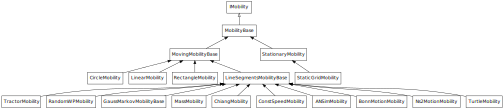
\includegraphics{figures/mobility_classes}
%\end{center}
%\end{figure}

% FIXME The Z coordinate is often initialized randomly.
%       It would be better (backward compatibility)
%       to initialize them to 0. (contsraintAreaDepth=0 not handled everywhere)


\section{Implemented models}

\subsection{Deterministic movements}

\begin{description}

\item[StationaryMobility] This mobility module does nothing;
it can be used for stationary nodes.

\item[StaticGridMobility] Places all nodes in a rectangular grid.

% TODO it always creates an N x N grid, generalize

\item[LinearMobility] This is a linear mobility model with speed,
angle and acceleration parameters. Angle only changes when the mobile
node hits a wall: then it reflects off the wall at the same angle.

z coordinate is constant
movement is always parallel with X-Y plane

% TODO interpret 'angle' as asimuth and introduce inclination angle (default is 0)
%      to describe movement along arbitrary line segment
% FIXME why different speed and lastSpeed

\item[CircleMobility] Moves the node around a circle parallel to the X-Y plane
with constant speed.
The node bounces from the bounds of the constraint area.
The circle is given by the \fpar{cx}, \fpar{cy} and \fpar{r} parameters,
The initial position determined by the \fpar{startAngle} parameter.
The position of the node is refreshed in \fpar{updateInterval} steps.

\item[RectangleMobility] Moves the node around the constraint area.
configuration: speed, startPos, updateInterval
% should be derived from LineSegmentsMobilityBase?

\item[TractorMobility] Moves a tractor through a field with a certain
amount of rows. The following figure illustrates the movement of the
tractor when the \fpar{rowCount} parameter is 2. The trajectory follows
the segments in $1,2,3,4,5,6,7,8,1,2,3\ldots$ order. The area is configured
by the \fpar{x1}, \fpar{y1}, \fpar{x2}, \fpar{y2} parameters.

% TODO use constraint area instead of new x1,y1,x2,y2 parameters as in RectangleMobility

\begin{center}
\setlength{\unitlength}{0.5mm}
\begin{picture}(80,80)
\put(40,72){$1$} \put(10,70){\vector(1,0){30}} \put(10,70){\line(1,0){60}}
\put(72,55){$2$} \put(70,70){\vector(0,-1){15}} \put(70,70){\line(0,-1){30}}
\put(40,42){$3$} \put(70,40){\vector(-1,0){30}} \put(70,40){\line(-1,0){60}}
\put(5,25){$4$} \put(10,40){\vector(0,-1){15}} \put(10,40){\line(0,-1){30}}
\put(40,12){$5$} \put(10,10){\vector(1,0){30}} \put(10,10){\line(1,0){60}}
\put(72,25){$6$} \put(70,10){\vector(0,1){15}} \put(70,10){\line(0,1){30}}
\put(40, 33){$7$}
\put(5,55){$8$} \put(10,40){\vector(0,1){15}} \put(10,40){\line(0,1){30}}
\put(0,72){$(x_1,y_1)$} \put(65,2){$(x_2,y_2)$}
\end{picture}
\end{center}

\end{description}

\subsection{Random movements}

\begin{description}

\item[RandomWPMobility]

In the Random Waypoint mobility model the nodes move in line segments. For each
line segment, a random destination position (distributed uniformly over the
playground) and a random speed is chosen. You can define a speed as a variate
from which a new value will be drawn for each line segment; it is customary to
specify it as \ttt{uniform(minSpeed, maxSpeed)}. When the node reaches the
target position, it waits for the time \fpar{waitTime} which can also be defined as a
variate. After this time the the algorithm calculates a new random position, etc.

\item[GaussMarkovMobility] The Gauss-Markov model contains a tuning
parameter, that control the randomness in the movement of the node.
Let the magnitude and direction of speed of the node at the $n$th time step be
$s_n$ and $d_n$. The next speed and direction is computed as

$$ s_{n+1} = \alpha s_n + (1 - \alpha) \bar{s} +
             \sqrt{(1-\alpha^2)} s_{x_n} $$

$$ d_{n+1} = \alpha s_n + (1 - \alpha) \bar{d} +
             \sqrt{(1-\alpha^2)} d_{x_n} $$

where $\bar{s}$ and $\bar{d}$ are constants representing the mean value
of speed and direction as $n \to \infty$; and $s_{x_n}$ and $d_{x_n}$
are random variables with Gaussian distribution.

Totally random walk (Brownian motion) is obtained by setting $\alpha=0$,
while $\alpha=1$ results a linear motion.

To ensure that the node does not remain at the boundary of the constraint
area for a long time, the mean value of the direction ($\bar{d}$) modified
as the node enters the margin area. For example at the right edge of the
area it is set to 180 degrees, so the new direction is away from the edge.

% FIXME the GaussMarkovMobility module has only one variance parameter.
%       it should have separate speed and direction parameters

\item[MassMobility]

This is a random mobility model for a mobile host with
a mass. It is the one used in \cite{Perkins99optimizedsmooth}.

\begin{quote}
"An MH moves within the room according to the following pattern. It moves
along a straight line for a certain period of time before it makes a turn.
This moving period is a random number, normally distributed with average of
5 seconds and standard deviation of 0.1 second. When it makes a turn, the
new direction (angle) in which it will move is a normally distributed
random number with average equal to the previous direction and standard
deviation of 30 degrees. Its speed is also a normally distributed random
number, with a controlled average, ranging from 0.1 to 0.45 (unit/sec), and
standard deviation of 0.01 (unit/sec). A new such random number is picked
as its speed when it makes a turn. This pattern of mobility is intended to
model node movement during which the nodes have momentum, and thus do not
start, stop, or turn abruptly. When it hits a wall, it reflects off the
wall at the same angle; in our simulated world, there is little other
choice."
\end{quote}

This implementation can be parameterized a bit more, via the
\fpar{changeInterval}, \fpar{changeAngleBy} and \fpar{changeSpeedBy} parameters.
The parameters described above correspond to the following settings:

\begin{inifile}
changeInterval = normal(5, 0.1)
changeAngleBy = normal(0, 30)
speed = normal(avgSpeed, 0.01)
\end{inifile}

\item[ChiangMobility] Chiang's random walk movement model
(\cite{Chiang98wirelessnetwork}).

In this model, the state of the mobile node in each direction (x and y) can be:

\begin{itemize}
  \item 0: the node stays in its current position
  \item 1: the node moves forward
  \item 2: the node moves backward
\end{itemize}

The $(i,j)$ element of the state transition matrix determines the
probability that the state changes from $i$ to $j$:

$$ \left(
\begin{array}{ccc}
  0 & 0.5 & 0.5 \\
  0.3 & 0.7 & 0 \\
  0.3 & 0 & 0.7
\end{array}
\right) $$

The \nedtype{ChiangMobility} module supports the following parameters:
\begin{itemize}
  \item \fpar{updateInterval} position update interval
  \item \fpar{stateTransitionInterval} state update interval
  \item \fpar{speed}: the speed of the node
\end{itemize}


% FIXME last line of setTargetPosition() contains a sign error, should be
%              targetPosition = lastPosition + lastSpeed * stateTransitionUpdateInterval;
% FIXME when reflecting at the boundary, state variables should be reflected too

\item[ConstSpeedMobility]

\nedtype{ConstSpeedMobility} does not use one of the standard mobility
approaches. The user can define a velocity for each Host and an update interval. If
the velocity is greater than zero (i.e. the Host is not stationary) the
\nedtype{ConstSpeedMobility} module calculates a random target position for the
Host. Depending to the update interval and the velocity it calculates the number of
steps to reach the destination and the step-size. Every update interval
\nedtype{ConstSpeedMobility} calculates the new position on its way to the
target position and updates the display. Once the target position is reached
\nedtype{ConstSpeedMobility} calculates a new target position.

This component has been taken over from Mobility Framework 1.0a5.

% FIXME this is a special case of RandomWPMobility, remove

\end{description}

\subsection{Replaying trace files}

\begin{description}

\item[BonnMotionMobility] Uses the native file format of
\href{http://www.cs.uni-bonn.de/IV/BonnMotion/}{BonnMotion}.

The file is a plain text file, where every line describes the motion
of one host. A line consists of one or more (t, x, y) triplets of real
numbers, like:

\begin{verbatim}
t1 x1 y1 t2 x2 y2 t3 x3 y3 t4 x4 y4 ...
\end{verbatim}

The meaning is that the given node gets to $(xk,yk)$ at $tk$. There's no
separate notation for wait, so x and y coordinates will be repeated there.

\item[Ns2Mobility] Nodes are moving according to the trace files used
in NS2.
The trace file has this format:

\begin{verbatim}
# '#' starts a comment, ends at the end of line
$node_(<id>) set X_ <x> # sets x coordinate of the node identified by <id>
$node_(<id>) set Y_ <y> # sets y coordinate of the node identified by <id>
$node_(<id>) set Z_ <z> # sets z coordinate (ignored)
$ns at $time "$node_(<id>) setdest <x> <y> <speed>" # at $time start moving
towards <x>,<y> with <speed>
\end{verbatim}

The \nedtype{Ns2MotionMobility} module has the following parameters:

\begin{itemize}
  \item \fpar{traceFile} the Ns2 trace file
  \item \fpar{nodeId} node identifier in the trace file; -1 gets substituted by
  parent module's index
  \item \fpar{scrollX},\fpar{scrollY} user specified translation of the
  coordinates
\end{itemize}

% TODO cleaning the code (e.g. duplicated bounds check in setTargetPosition())
% TODO implement cached file access as in BonnMotionMobility

\item[ANSimMobility] reads trace files of the \href{http://www.ansim.info}{ANSim} Tool.

The nodes are moving along linear segments described by an XML trace file
conforming to this DTD:

\begin{verbatim}
<!ELEMENT mobility (position_change*)>
<!ELEMENT position_change (node_id, start_time, end_time, destination)>
<!ELEMENT node_id (#PCDATA)>
<!ELEMENT start_time (#PCDATA)>
<!ELEMENT end_time (#PCDATA)>
<!ELEMENT destination (xpos, ypos)>
<!ELEMENT xpos (#PCDATA)>
<!ELEMENT ypos (#PCDATA)>
\end{verbatim}

Parameters of the module:

\begin{itemize}
  \item \fpar{ansimTrace} the trace file
  \item \fpar{nodeId} the \verb!node_id! of this node, -1 gets substituted to
  parent module's index
\end{itemize}

\begin{note}
The \nedtype{ANSimMobility} module process only the \ttt{position\_{}change}
elements and it ignores the \ttt{start\_{}time} attribute. It starts the move
on the next segment immediately.
\end{note}


\end{description}




\section{Mobility scripts}

The \nedtype{TurtleMobility} module can be parametrized by a script file
containing LOGO-style movement commands in XML format.

The module has these parameters:

\begin{itemize}
\item \ttt{updateInterval} time interval to update the hosts position
\item \ttt{constraintAreaX}, \ttt{constraintAreaY}, \ttt{constraintAreaWidth},
      \ttt{constraintAreaHeight}: constraint area that the node can not leave
\item \ttt{turtleScript} XML file describing the movements
\end{itemize}

The content of the XML file should conform to the following DTD (can be
found as \ffilename{TurtleMobility.dtd} in the source tree):

\begin{verbatim}
<!ELEMENT movements (movement)*>

<!ELEMENT movement (repeat|set|forward|turn|wait|moveto|moveby)*>
<!ATTLIST movement id NMTOKEN #IMPLIED>

<!ELEMENT repeat (repeat|set|forward|turn|wait|moveto|moveby)*>
<!ATTLIST repeat n CDATA #IMPLIED>

<!ELEMENT set EMPTY>
<!ATTLIST set x     CDATA #IMPLIED
              y     CDATA #IMPLIED
              speed CDATA #IMPLIED
              angle CDATA #IMPLIED
              borderPolicy (reflect|wrap|placerandomly|error) #IMPLIED>

<!ELEMENT forward EMPTY>
<!ATTLIST forward d CDATA #IMPLIED
                  t CDATA #IMPLIED>

<!ELEMENT turn EMPTY>
<!ATTLIST turn angle CDATA #REQUIRED>

<!ELEMENT wait EMPTY>
<!ATTLIST wait t CDATA #REQUIRED>

<!ELEMENT moveto EMPTY>
<!ATTLIST moveto x CDATA #IMPLIED
                 y CDATA #IMPLIED
                 t CDATA #IMPLIED>

<!ELEMENT moveby EMPTY>
<!ATTLIST moveby x CDATA #IMPLIED
                 y CDATA #IMPLIED
                 t CDATA #IMPLIED>
\end{verbatim}

The file contains \ttt{movement} elements, each describing a trajectory.
The \ttt{id} attribute of the \ttt{movement} element can be used to
refer the movement from the ini file using the syntax:

\begin{inifile}
**.mobility.turtleScript = xmldoc("turtle.xml", "movements//movement[@id='1']")
\end{inifile}

The motion of the node is composed of uniform linear segments.
The state of motion is described by the following variables:
\begin{itemize}
\item \ttt{position}: $(x,y)$ coordinate of the current location of the node
\item \ttt{speed}, \ttt{angle}: magnitude and direction of the node's velocity
\item \ttt{targetPos}: target position of the current line segment. If given
                       the \ttt{speed} and \ttt{angle} is not used
\item \ttt{targetTime} the end time of the current linear motion
\item \ttt{borderPolicy}: one of
    \begin{itemize}
      \item \ttt{reflect} the node reflects at the boundary,
      \item \ttt{wrap} the node appears at the other side of the area,
      \item \ttt{placerandomly} the node placed at a random position of the area,
      \item \ttt{error} signals an error when the node reaches the boundary
    \end{itemize}
\end{itemize}

The \ttt{movement} elements may contain the the following commands:

\begin{itemize}
\item \ttt{repeat(n)} repeats its content n times, or indefinetly if the n attribute
              is omitted.
\item \ttt{set(x,y,speed,angle,borderPolicy)} modifies the state of the node.
\item \ttt{forward(d,t)} moves the node for $t$ time or to the $d$ distance
with the current speed. If both $d$ and $t$ is given, then the current
speed is ignored.
\item \ttt{turn(angle)} increase the angle of the node by $angle$ degrees.
\item \ttt{moveto(x,y,t)} moves to point $(x,y)$ in the given time. If
$t$ is not specified, it is computed from the current speed.
\item \ttt{moveby(x,y,t)} moves by offset $(x,y)$ in the given time. If
$t$ is not specified, it is computed from the current speed.
\item \ttt{wait(t)} waits for the specified amount of time.
\end{itemize}

Attribute values must be given without physical units, distances are assumed
to be given as meters, time intervals in seconds and speeds in meter per seconds.
Attibutes can contain expressions that are evaluated each time the
command is executed. The limits of the constraint area can be
referenced as \verb!$MINX!, \verb!$MAXX!, \verb!$MINY!, and \verb!$MAXY!.
Random number distibutions generate a new random number when evaluated,
so the script can describe random as well as deterministic scenarios.

To illustrate the usage of the module, we show how some mobility
models can be implemented as scripts:

\begin{itemize}
\item RectangleMobility:

\begin{verbatim}
    <movement>
        <set x="$MINX" y="$MINY" angle="0" speed="10"/>
        <repeat>
            <repeat n="2">
                <forward d="$MAXX-$MINX"/>
                <turn angle="90"/>
                <forward d="$MAXY-$MINY"/>
                <turn angle="90"/>
            </repeat>
        </repeat>
    </movement>
\end{verbatim}

\item Random Waypoint:

\begin{verbatim}
    <movement>
        <repeat>
            <set speed="uniform(20,60)"/>
            <moveto x="uniform($MINX,$MAXX)" y="uniform($MINY,$MAXY)"/>
            <wait t="uniform(5,10)">
        </repeat>
    </movement>
\end{verbatim}

\item MassMobility:

\begin{verbatim}
    <movement>
        <repeat>
            <set speed="uniform(10,20)"/>
            <turn angle="uniform(-30,30)"/>
            <forward t="uniform(0.1,1)"/>
        </repeat>
    </movement>
\end{verbatim}

\end{itemize}


%%% Local Variables:
%%% mode: latex
%%% TeX-master: "usman"
%%% End:



\cleardoublepage

% based on 'integration' branch: 446a1265c28822456bc0230d362bbabdee7778ba (2012-03-19)

\chapter{IPv4}
\label{cha:ipv4}


\section{Overview}

The IP protocol is the workhorse protocol of the TCP/IP protocol suite.
All UDP, TCP, ICMP packets are encapsulated into IP datagrams and
transported by the IP layer.
While higher layer protocols transfer data among two communication end-point,
the IP layer provides an hop-by-hop, unreliable and connectionless delivery
service. IP does not maintain any state information about the individual
datagrams, each datagram handled independently.

The nodes that are connected to the Internet can be either a host or a router.
The hosts can send and recieve IP datagrams, and their operating system
implements the full TCP/IP stack including the transport layer. On the
other hand, routers have more than one interface cards and perform packet
routing between the connected networks. Routers does not need the
transport layer, they work on the IP level only. The division
between routers and hosts is not strict, because if a host
have several interfaces, they can usually be configured to operate
as a router too.

Each node on the Internet has a unique IP address. IP datagrams contain
the IP address of the destination. The task of the routers is to find
out the IP address of the next hop on the local network, and forward
the packet to it. Sometimes the datagram is larger, than the maximum
datagram that can be sent on the link (e.g. Ethernet has an 1500 bytes limit.).
In this case the datagram is split into fragments and each fragment is
transmitted independently. The destination host must collect all fragments,
and assemble the datagram, before sending up the data to the transport
layer.

\subsection{INET modules}

The INET framework contains several modules to build the
IPv4 network layer of hosts and routers:
\begin{itemize}
  \item \nedtype{IPv4} is the main module that implements RFC791. This
        module performs IP encapsulation/decapsulation, fragmentation
        and assembly, and routing of IP datagrams.
  \item The \nedtype{IPv4RoutingTable} is a helper module that manages the routing
        table of the node. It is queried by the \nedtype{IPv4} module
        for best routes, and updated by the routing daemons implementing
        RIP, OSPF, Manet, etc. protocols.
  \item The \nedtype{ICMP} module can be used to generate ICMP error packets. It also
        supports ICMP echo applications.
  \item The \nedtype{ARP} module performs the dynamic translation of IP addresses
        to MAC addresses.
  \item The \nedtype{IGMPv2} module to generate and process multicast group
        membership reports.
\end{itemize}

These modules are assembled into a complete network layer module
called \nedtype{IPv4NetworkLayer}. This module has
dedicated gates for TCP, UDP, SCTP, RSVP, OSPF, Manet, and Ping
higher layer protocols. It can be connected to several network
interface cards: Ethernet, PPP, Wlan, or external interfaces.
The \nedtype{IPv4NetworkLayer} module is used to build IPv4 hosts
(\nedtype{StandardHost}) and routers (\nedtype{Router}).

The implementation of these modules are based on the following RFCs:
\begin{itemize}
  \item RFC791: Internet Protocol
  \item RFC792: Internet Control Message Protocol
  \item RFC826: Address Resolution Protocol
  \item RFC1122: Requirements for Internet Hosts - Communication Layers
  \item RFC2236: Internet Group Management Protocol, Version 2
\end{itemize}

The subsequent sections describe the IPv4 modules in detail.

\section{The IPv4 Module}

The \nedtype{IPv4} module implements the IPv4 protocol.

For connecting the upper layer protocols the \nedtype{IPv4} module
has \emph{transportIn[]} and \emph{transportOut[]} gate vectors.

The IP packets are sent to the \nedtype{ARP} module through the
\emph{queueOut} gate. The incoming IP packets are received
directly from the network interface cards through the
\emph{queueIn[]} gates. Each interface card knows its own
network layer gate index.


\subsection{IP packets}

IP datagrams start with a variable length IP header.
The minimum length of the header is 20 bytes, and
it can contain at most 40 bytes for options, so
the maximum length of the IP header is 60 bytes.

\begin{center}
\begin{bytefield}{32}
\bitheader{0,3,4,7,8,15,16,18,19,23,24,31} \\
\bitbox{4}{Version} &
\bitbox{4}{IHL} &
\bitbox{8}{\small Type of Service} &
\bitbox{16}{Total Length} \\
\bitbox{16}{Identification} &
\bitbox{3}{Flags} &
\bitbox{13}{Fragment Offset} \\
\bitbox{8}{Time to Live} &
\bitbox{8}{Protocol} &
\bitbox{16}{Header Checksum} \\
\bitbox{32}{Source Address} \\
\bitbox{32}{Destination Address} \\
\bitbox{24}{Options} &
\bitbox{8}{Padding} \\
\end{bytefield}
\end{center}

The \ttt{Version} field is 4 for IPv4. The 4-bit \ttt{IHL} field is the
number of 32-bit words in the header. It is needed because the header
may contain optional fields, so its length may vary. The minimum IP header
length is 20, the maximum length is 60. The header is always padded to
multiple of 4 bytes. The \ttt{Type of Service} field designed to store
priority and preference values of the IP packet, so applications can
request low delay, high throughput, and maximium reliability from the
routing algorithms. In reality these fields are rarely set by applications,
and the routers mostly ignore them. The \ttt{Total Length} field is the
length of the whole datagram in bytes. The \ttt{Identification} field
is used for identifying the datagram sent by a host. It is usually generated
by incrementing a counter for each outgoing datagram. When the datagram
gets fragmented by a router, its \ttt{Identification} field is kept unchanged
to the other end can collect them. In datagram fragments the \ttt{Fragment Offset}
is the address of the fragment in the payload of the original datagram. It is
measured in 8-byte units, so fragment lengths must be a multiple of 8.
Each fragment except the last one, has its \ttt{MF} (more fragments) bit set
in the \ttt{Flags} field. The other used flag in \ttt{Flags} is the \ttt{DF}
(don't fragment) bit which forbids the fragmentation of the datagram.
The \ttt{Time to Live} field is decremented by each router in the path,
and the datagram is dropped if it reached 0. Its purpose is to prevent
endless cycles if the routing tables are not properly configured, but
can be used for limiting hop count range of the datagram (e.g. for local
broadcasts, but the \fprog{traceroute} program uses this field too).
The \ttt{Protocol} field is for demultiplexing the payload of the IP
datagram to higher level protocols. Each transport protocol has a registered
protocol identifier. The \ttt{Header Checksum} field is the 16-bit one's
complement sum of the header fields considered as a sequence of 16-bit numbers.
The \ttt{Source Address} and \ttt{Destination Address} are the IPv4 addresses
of the source and destination respectively.

The \ttt{Options} field contains 0 or more IP options. It is always padded
with zeros to a 32-bit boundary. An option is either a single-byte option
code or an option code + option length followed by the actual values for
the option. Thus IP implementations can skip unknown options.

An IP datagram is represented by the \msgtype{IPv4Datagram} message class.
It contains variables corresponding the fields of the IP header, except:
\begin{itemize}
  \item \fvar{Header Checksum} omitted, modeled by error bit of packets
  \item \fvar{Options} only the following options are permitted and the
                       datagram can contain at most one option:
        \begin{itemize}
          \item Loose Source Routing
          \item Strict Source Routing
          \item Timestamp
          \item Record Route
        \end{itemize}
\end{itemize}

The \fvar{Type of Service} field is called \ttt{diffServCodePoint} in
\nedtype{IPv4Datagram}.

Before sending the \msgtype{IPv4Datagram} through the network, the \nedtype{IPv4}
module attaches a \cppclass{IPv4RoutingDecision} control info.
The control info contains the IP address of the next hop, and the
identifier of the interface it should be sent. The ARP module translate
the IP address to the hardware address on the local net of the specified
interface and forwards the datagram to the interface card.


\subsection{Parameters}

The \nedtype{IPv4} module has the following parameters:
\begin{itemize}
  \item \fpar{procDelay} processing time of each incoming datagram.
  \item \fpar{timeToLive} default TTL of unicast datagrams.
  \item \fpar{multicastTimeToLive} default TTL of multicast datagrams.
  \item \fpar{protocolMapping} string value containing the \ttt{protocol id}
        $\rightarrow$ \ttt{gate index} mapping, e.g. \ttt{``6:0,17:1,1:2,2:3,46:4''}.
  \item \fpar{fragmentTimeout} the maximum duration until fragments are kept
          in the fragment buffer.
  \item \fpar{forceBroadcast} if \fkeyword{true}, then link-local broadcast
          datagrams are sent out through each interface, if the higher
          layer did not specify the outgoing interface.
\end{itemize}

% compile time options: WITH\_MANET, NEWFRAGMENT

\subsection{Statistics}

The \nedtype{IPv4} module does not write any statistics into files,
but it has some statistical information that can be watched during
the simulation in the gui environment.
\begin{itemize}
  \item \ttt{numForwarded}: number of forwarded datagrams, i.e. sent to one of the
        interfaces (not broadcast), counted before fragmentation.
  \item \ttt{numLocalDeliver}: number of datagrams locally delivered.
        (Each fragment counted separately.)
  \item \ttt{numMulticast}: number of routed multicast datagrams.
  \item \ttt{numDropped} number of dropped packets.
        Either because there is no any interface, the interface is not specified and
        no \fpar{forceBroadcast}, or received from the network but IP forwarding disabled.
  \item \ttt{numUnroutable}: number of unroutable datagrams, i.e. there is no
        route to the destination. (But if outgoing interface is specified it is routed!)
\end{itemize}

In the graphical interface the bubble of the \nedtype{IPv4} module
also displays these counters.


\section{The IPv4RoutingTable module}

The \nedtype{IPv4RoutingTable} module represents the routing table.
IP hosts and routers contain one instance of this class. It has
methods to manage the routing table and the interface table,
so one can achieve functionality similar to the \fprog{route} and
\fprog{ifconfig} commands.

This is a simple module without gates, it requires function calls to it
(message handling does nothing). Methods are provided for reading and
updating the interface table and the route table, as well as for unicast
and multicast routing.

\subsection*{Parameters}

The \nedtype{IPv4RoutingTable} module has the following parameters:

\begin{itemize}
  \item \fpar{routerId}: for routers, the router id using IPv4 address dotted notation;
        specify ``auto'' to select the highest interface address; should be left empty ``''
        for hosts
  \item \fpar{IPForward}: turns IP forwarding on/off (It is always \fkeyword{true}
                          in a \nedtype{Router} and is \fkeyword{false} by default
                          in a \nedtype{StandardHost}.)
  \item \fpar{forwardMulticast}: turns multicast IP forwarding on/off. Default is \fkeyword{false},
  should be set to \fkeyword{true} in multicast routers.
  \item \fpar{routingFile}: name of routing file that configures IP addresses and routes of the node
  containing this routing table. Its format is described in section \ref{subsec:routing_files}.
\end{itemize}

\begin{warning}
The \fpar{routingFile} parameter is obsolete. The prefered method for network configuration
is to use \nedtype{IPv4NetworkConfigurator}. The old config files should be replaced
with the XML configuration of \nedtype{IPv4NetworkConfigurator}. Section \ref{subsec:ipv4configurator}
describes the format of the new configuration files.
\end{warning}

% FIXME (#467) IPv4RoutingTable::invalidateCache() should clear localBroadcastAddresses.
% IPv4RoutingTable::findBestMatchingRoute() should search in this order:
%          1. host routes (exact match)
%          2. network routes (longest match)
%          3. default routes (round robin)
%   It is ok, if host routes has 255.255.255.255 netmask, and default has 0.0.0.0 netmask.
% FIXME IPv4RoutingTable::findBestMatchingRoute() if(...MANET...) branch always set bestRoute to NULL,
%       because if there were exact match, it would have been choosen in the previous loop.

\section{The ICMP module}

The Internet Control Message Protocol (ICMP) is the error reporting and
diagnostic mechanism of the Internet.
It uses the services of IP, so it is a transport layer protocol, but unlike
TCP or UDP it is not used to transfer user data. It can not be separated
from the IP, because the routing errors are reported by ICMP.

The \nedtype{ICMP} module can be used to send error messages and ping
request. It can also respond to incoming ICMP messages.

Each ICMP message is encapsulated within an IP datagram, so its delivery
is unreliable.

\begin{center}
\begin{bytefield}{32}
\bitheader{0,7,8,15,31} \\
\bitbox{8}{Type} &
\bitbox{8}{Code} &
\bitbox{16}{Checksum} \\
\bitbox{32}{Rest of header} \\
\wordbox{2}{Internet Header + 8 bytes of Original Datagram}
\end{bytefield}
\end{center}

The corresponding message class (\msgtype{ICMPMessage}) contains only
the Type and Code fields. The message encapsulates the IP packet that
triggered the error, or the data of the ping request/reply.

% FIXME type=PARAMETER_PROBLEM, code=0: missing Pointer field from ICMPMessage
%            REDIRECT: Gateway Internet Address
%            ECHO_REQUEST, ECHO_REPLY: Identifier, Sequence Number
%            TIMESTAMP_REQUEST, TIMESTAMP_REPLY: Identifier, Sequence Number, Originate Timestamp, Receive Timestamp, Transmit Timestamp

% FIXME wrong type codes for ICMP_DESTINATION_UNREACHABLE (3), ICMP_ECHO_REQUEST (8), ICMP_ECHO_REPLY (0), ICMP_TIMESTAMP_REQUEST (13), ICMP_TIMESTAMP_REPLY (14)

% FIXME ICMP header serializer handles only ICMP_ECHO_REQUEST, ICMP_ECHO_REPLY, ICMP_DESTINATION_UNREACHABLE, ICMP_TIME_EXCEEDED
%       ICMP header deserializer handles only ICMP_ECHO_REQUEST, ICMP_ECHO_REPLY

% FIXME ICMP error should not be send if the original datagram
%         1. is an ICMP error
%         2. was sent to a broadcast or multicast address
%         3. datagram was sent with a link-layer broadcast
%         4. a fragment other than the first
%         5. a datagram whose source address is 0.0.0.0, 127.*.*.*, broadcast or multicast address
%      currently only the 1. and half of 2. checked


% \section{The IGMP module}

\section{The ARP module}

The \nedtype{ARP} module implements the Address Resolution Protocol (RFC826).
The ARP protocol is designed to translate a local protocol address
to a hardware address. Altough the ARP protocol can be used with
several network protocol and hardware addressing schemes, in practice
they are almost always IPv4 and 802.3 addresses. The INET implementation
of the ARP protocol (the \nedtype{ARP} module) supports only
IP address $\rightarrow$ MAC address translation.

If a node wants to send an IP packet to a node whose MAC address is unknown,
it broadcasts an ARP frame on the Ethernet network.
In the request its publish its own IP and
MAC addresses, so each node in the local subnet can update their mapping.
The node whose MAC address was requested will respond with an ARP frame
containing its own MAC address directly to the node that sent the
request. When the original node receives the ARP response, it updates
its ARP cache and sends the delayed IP packet using the learned MAC address.

The frame format of the ARP request and reponse is shown in Figure \ref{fig:ARP_frame}.
In our case the HTYPE (hardware type), PTYPE (protocol type), HLEN (hardware address length)
and PLEN (protocol address length) are constants: HTYPE=Ethernet (1), PTYPE=IPv4 (2048), HLEN=6,
PLEN=4. The OPER (operation) field is 1 for an ARP request and 2 for an ARP response.
The SHA field contains the 48-bit hardware address of the sender, SPA field is
the 32-bit IP address of the sender; THA and TPA are the addresses of the target.
The message class corresponding to the ARP frame is \msgtype{ARPPacket}.
In this class only the OPER, SHA, SPA, THA and TPA fields are stored.
The length of an \msgtype{ARPPacket} is 28 bytes.

\begin{figure}[h]
\begin{center}
\label{fig:ARP_frame}
\begin{bytefield}{16}
\bitheader{0,7,8,15} \\
\bitbox{16}{HTYPE} \\
\bitbox{16}{PTYPE} \\
\bitbox{8}{HLEN} &
\bitbox{8}{PLEN} \\
\bitbox{16}{OPER} \\
\wordbox{3}{SHA} \\
\wordbox{2}{SPA} \\
\wordbox{3}{THA} \\
\wordbox{2}{TPA} \\
\end{bytefield}
\caption{ARP frame}
\end{center}
\end{figure}

The \nedtype{ARP} module receives IP datagrams and ARP responses from \nedtype{IPv4}
on the \ttt{ipIn} gate and transmits IP datagrams and ARP requests on the \ttt{nicOut[]} gates
towards the network interface cards. ARP broadcasts the requests on the local network,
so the NIC's entry in the \nedtype{InterfaceTable} should have \ffunc{isBroadcast()} flag
set in order to participate in the address resolution.

The incoming IP packet should have an attached \cppclass{IPv4RoutingDecision} control
info containing the IP address of the next hop. The next hop can be either an
IPv4 broadcast/multicast or a unicast address. The corresponding MAC addresses
can be computed for broadcast and multicast addresses (RFC 1122, 6.4); unicast
addresses are mapped using the ARP procotol.

If the hardware address is found
in the ARP cache, then the packet is transmitted to the addressed interface immediately.
Otherwise the packet is queued and an address resolution takes place.
The \nedtype{ARP} module creates an \msgtype{ARPPacket} object, sets the sender
MAC and IP address to its own address, sets the destination IP address
to the address of the target of the IP datagram, leave the destination MAC address
blank and broadcasts the packet on each network interface with broadcast capability.
Before sending the ARP packet, it retransmission a timer. If the timer expires,
it will retransmit the ARP request, until the maximum retry count is reached.
If there is no response to the ARP request, then the address resolution fails,
and the IP packet is dropped from the queue. Otherwise the MAC address of the
destination is learned and the IP packet can be transmitted on the corresponding
interface.

When an ARP packet is received on the \ttt{ipIn} gate, and the sender's IP
is already in the ARP cache, it is updated with the information in the ARP frame.
Then it is checked that the destination IP of the packet matches with our
address. In this case a new entry is created with the sender addresses in the
ARP cache, and if the packet is a request a response is created and sent directly
to the originator. If proxy ARP is enabled, the request can be responded
with our MAC address if we can route IP packets to the destination.

Usually each \nedtype{ARP} module maintains a local ARP cache.
However it is possible to use a global cache. The global cache is filled
in with entries of the IP and MAC addresses of the known interfaces
when the ARP modules are initiated (at simulation time 0).
\nedtype{ARP} modules that are using the global ARP cache
never initiate an address resolution; if an IP address not
found in the global cache, the simulation stops with an error.
However they will respond to ARP request, so the simulation can
be configured so that some \nedtype{ARP}s use local, while others
the global cache.

When an entry is inserted or updated in the local ARP cache,
the simulation time saved in the entry. The mapping in the
entry is not used after the configured \fpar{cacheTimeout}
elapsed. This parameter does not affect the entries of
the global cache however.

The module parameters of \nedtype{ARP} are:

\begin{itemize}
  \item \fpar{retryTimeout}: number of seconds ARP waits between retries to resolve an IPv4 address (default is 1s)
  \item \fpar{retryCount}: number of times ARP will attempt to resolve an IPv4 address (default is 3)
  \item \fpar{cacheTimeout}: number of seconds unused entries in the cache will time out (default is 120s)
  \item \fpar{proxyARP}: enables proxy ARP mode (default is \fkeyword{true})
  \item \fpar{globalARP}: use global ARP cache (default is \fkeyword{false})
\end{itemize}

The \nedtype{ARP} module emits four signals:

\begin{itemize}
  \item \ttt{sentReq}: emits 1 each time an ARP request is sent
  \item \ttt{sentReplies}: emits 1 each time an ARP response is sent
  \item \ttt{initiatedResolution}: emits 1 each time an ARP resolution is initiated
  \item \ttt{failedResolution}: emits 1 each time an ARP resolution is failed
\end{itemize}

These signals are recorded as vectors and their counts as scalars.

% TODO watches, animation effects

\section{The IGMP module}

The IGMP module is responsible for distributing the information of
multicast group memberships from hosts to routers. When an interface
of a host joins to a multicast group, it will send an IGMP report
on that interface to routers. It can also send reports when the
interface leaves the multicast group, so it does not want to
receive those multicast datagrams. The IGMP module of multicast
routers processes these IGMP reports: it updates the list of
groups, that has members on the link of the incoming message.

The \nedtype{IIGMP} module interface defines the connections
of IGMP modules.
IGMP reports are transmitted by IP, so the module contains
gates to be connected to the IP module (\ttt{ipIn/ipOut}). The IP
module delivers packets with protocol number 2 to the IGMP module.
However some multicast routing protocols (like DVMRP) also exchange
routing information by sending IGMP messages, so they should be
connected to the \ttt{routerIn/routerOut} gates of the IGMP module.
The IGMP module delivers the IGMP messages not processed by itself
to the connected routing module.

The \nedtype{IGMPv2} module implements version 2 of the IGMP protocol
(RFC 2236). Next we describe its behaviour in host and routers in details.
Note that multicast routers behaves as hosts too, i.e. they are sending
reports to other routers when joining or leaving a multicast group.

\subsection{Host behaviour}

When an interface joins to a multicast group, the host
will send a Membership Report immediately to the group address.
This report is repeated after \fpar{unsolicetedReportInterval} to
cover the possibility of the first report being lost.

When a host's interface leaves a multicast group, and it was
the last host that sent a Membership Report for that group,
it will send a Leave Group message to the all-routers multicast
group (224.0.0.2).

This module also responds to IGMP Queries. When the host
receives a Group-Specific Query on an interface that belongs
to that group, then it will set a timer to a random value
between 0 and Max Response Time of the Query. If the timer
expires before the host observe a Membership Report sent
by other hosts, then the host sends an IGMPv2 Membership Report.
When the host receives a General Query on an interface,
a timer is initialized and a report is sent for each group
membership of the interface.

\subsection{Router behaviour}

Multicast routers maintains a list for each interface containing
the multicast groups that have listeners on that interface.
This list is updated when IGMP Membership Reports and Leave Group
messages arrive, or when a timer expires since the last Query.

When multiple routers are connected to the same link, the one with
the smallest IP address will be the Querier. When other routers
observe that they are Non-Queriers (by receiving an IGMP Query
with a lower source address), they stop sending IGMP Queries
until \fpar{otherQuerierPresentInterval} elapsed since the last
received query.

Routers periodically (\fpar{queryInterval}) send a General Query
on each attached network for which this router is a Querier.
On startup the router sends \fpar{startupQueryCount} queries
separated by \fpar{startupQueryInterval}. A General Query
has unspecified Group Address field, a Max Response Time
field set to \fpar{queryResponseInterval}, and is sent to the
all-systems multicast address (224.0.0.1).

When a router receives a Membership Report, it will add the
reported group to the list of multicast group memberships.
At the same time it will set a timer for the membership
to \fpar{groupMembershipInterval}. Repeated reports restart
the timer. If the timer expires, the router assumes
that the group has no local members, and multicast traffic
is no more forwarded to that interface.

When a Querier receives a Leave Group message for a group,
it sends a Group-Specific Query to the group being left.
It repeats the Query \fpar{lastMemberQueryCount} times in
separated by \fpar{lastMemberQueryInterval} until a Membership
Report is received. If no Report received, then the router
assumes that the group has no local members.

% FIXME IGMPv2 not compatible with IGMPv1 hosts and routers

\subsection{Disabling IGMP}

The IPv4 \nedtype{IPv4NetworkLayer} contains an instance of the IGMP
module. IGMP can be turned off by setting the \fpar{enabled}
parameter to false. When disabled, then no IGMP message
is generated, and incoming IGMP messages are ignored.

\subsection{Parameters}

The following parameters has effects in both hosts and routers:

\begin{itemize}
  \item \fpar{enabled} if \fkeyword{false} then the IGMP module is silent. Default is \fkeyword{true}.
\end{itemize}

These parameters are only used in hosts:

\begin{itemize}
  \item \fpar{unsolicitedReportInterval} the time between repetitions of a
   host's initial report of membership in a group. Default is 10s.
\end{itemize}

Router timeouts are configured by these parameters:

\begin{itemize}
  \item \fpar{robustnessVariable} the IGMP is robust to \fpar{robustnessVariable}-1
   packet losses. Default is 2.
  \item \fpar{queryInterval} the interval between General Queries sent by a Querier.
   Default is 125s.
  \item \fpar{queryResponseInterval} the Max Response Time inserted into General Queries
  \item \fpar{groupMembershipInterval} the amount of time that must pass before
   a multicast router decides there are no more members of a group on a network.
   Fixed to \fpar{robustnessVariable} * \fpar{queryInterval} + \fpar{queryResponseInterval}.
  \item \fpar{otherQuerierPresentInterval} the length of time that must
   pass before a multicast router decides that there is no longer
   another multicast router which should be the querier.
   Fixed to \fpar{robustnessVariable} * \fpar{queryInterval} + \fpar{queryResponseInterval} / 2.
  \item \fpar{startupQueryInterval} the interval between General Queries
   sent by a Querier on startup. Default is \fpar{queryInterval} / 4.
  \item \fpar{startupQueryCount} the number of Queries sent out on startup,
   separated by the \fpar{startupQueryInterval}. Default is \fpar{robustnessVariable}.
  \item \fpar{lastMemberQueryInterval} the Max Response Time inserted into
   Group-Specific Queries sent in response to Leave Group messages, and
   is also the amount of time between Group-Specific Query messages.
   Default is 1s.
  \item \fpar{lastMemberQueryCount} the number of Group-Specific Queries
   sent before the router assumes there are no local members.
   Default is \fpar{robustnessVariable}.
\end{itemize}

\section{The IPv4NetworkLayer module}

The \nedtype{IPv4NetworkLayer} module packs the \nedtype{IP}, \nedtype{ICMP},
\nedtype{ARP}, and \nedtype{IGMP} modules into one compound module.
The compound module defines gates for connecting UDP, TCP, SCTP, RSVP and
OSPF transport protocols. The \ttt{pingIn} and \ttt{pingOut} gates of the
\nedtype{ICMP} module are also available, while its \ttt{errorOut} gate
is connected to an inner \nedtype{ErrorHandling} component that writes
the ICMP errors to the log.

The component can be used in hosts and routers to support IPv4.

\section{The NetworkInfo module}

The \nedtype{NetworkInfo} module can be used to dump detailed information
about the network layer. This module does not send or received messages,
it is invoked by the \nedtype{ScenarioManager} instead. For example
the following \nedtype{ScenarioManager} script dump the routing table
of the \ttt{LSR2} module at simulation time $t=2$ into \ffilename{LSR2\_002.txt}:
\begin{filelisting}
<scenario>
  <at t="2">
    <routing module="NetworkInfo" target="LSR2" file="LSR2_002.txt"/>
  </at>
</scenario>
\end{filelisting}

The module currently support only the \ttt{routing} command which dumps
the routing table. The command has four parameters given as XML attributes:
\begin{itemize}
  \item \ttt{target} the name of the node that owns the routing table to be dumped
  \item \ttt{filename} the name of the file the output is directed to
  \item \ttt{mode} if set to ``a'', the output is appended to the file,
                   otherwise the target is truncated if the file existed
  \item \ttt{compat} if set to ``linux'', then the output is generated
                     in the format of the \ttt{route -n} command of Linux.
                     The output is sorted only if \ttt{compat} is
                     \fkeyword{true}.
\end{itemize}

\section{Configuring IPv4 networks}

An IPv4 network is composed of several nodes like hosts, routers,
switches, hubs, Ethernet buses, or wireless access points.
The nodes having a IPv4 network layer (hosts and routers) should be
configured at the beginning of the simulation. The configuration
assigns IP addresses to the nodes, and fills their routing tables.
If multicast forwarding is simulated, then the multicast routing
tables also must be filled in.

% TODO define nodes, IP nodes, routers, multicast routers

The configuration can be manual (each address and route is fully specified
by the user), or automatic (addresses and routes are generated by
a configurator module at startup).

Before version 1.99.4 INET offered \nedtype{FlatNetworkConfigurator}
for automatic and routing files for manual configuration.
Both had serious limitations, so a new configurator has been added
in version 1.99.4: \nedtype{IPv4NetworkConfigurator}. This configurator
supports both fully manual and fully automatic configuration. It
can also be used with partially specified manual configurations,
the configurator fills in the gaps automatically.

The next section describes the usage of \nedtype{IPv4NetworkConfigurator},
\nedtype{FlatNetworkConfigurator} and old routing files are described
in the following sections.

\subsection{IPv4NetworkConfigurator}
\label{subsec:ipv4configurator}

The \nedtype{IPv4NetworkConfigurator} assigns IP addresses and sets up
static routing for an IPv4 network.

It assigns per-interface IP addresses, strives to take subnets into account,
and can also optimize the generated routing tables by merging routing entries.

Hierarchical routing can be set up by using only a fraction of configuration
entries compared to the number of nodes. The configurator also does
routing table optimization that significantly decreases the size of routing
tables in large networks.

The configuration is performed in stage 2 of the initialization. At this
point interface modules (e.g. PPP) has already registered their interface
in the interface table. If an interface is named \ttt{ppp[0]}, then the
corresponding interface entry is named \ttt{ppp0}. This name can be used
in the config file to refer to the interface.

The configurator goes through the following steps:
\begin{enumerate}
  \item  Builds a graph representing the network topology. The graph
     will have a vertex for every module that has a @node property (this
     includes hosts, routers, and L2 devices like switches, access points,
     Ethernet hubs, etc.) It also assigns weights to vertices and edges that
     will be used by the shortest path algorithm when setting up routes.
     Weights will be infinite for IP nodes that have IP forwarding disabled
     (to prevent routes from transiting them), and zero for all other nodes
     (routers and and L2 devices). Edge weights are chosen to be inversely
     proportional to the bitrate of the link, so that the configurator
     prefers connections with higher bandwidth. For internal purposes,
     the configurator also builds a table of all "links" (the link data
     structure consists of the set of network interfaces that are
     on the same point-to-point link or LAN)

  \item  Assigns IP addresses to all interfaces of all nodes. The
     assignment process takes into consideration the addresses and netmasks
     already present on the interfaces (possibly set in earlier initialize
     stages), and the configuration provided in the XML format (described
     below). The configuration can specify "templates" for the address
     and netmask, with parts that are fixed and parts that can be chosen
     by the configurator (e.g. "10.0.x.x"). In the most general case,
     the configurator is allowed to choose any address and netmask for all
     interfaces (which results in automatic address assignment). In the most
     constrained case, the configurator is forced to use the requested addresses
     and netmasks for all interfaces (which translates to manual address assignment).
     There are many possible configuration options between these two extremums. The
     configurator assigns addresses in a way that maximizes the number of
     nodes per subnet. Once it figures out the nodes that belong to a single
     subnet it, will optimize for allocating the longest possible netmask.
     The configurator might fail to assign netmasks and addresses according
     to the given configuration parameters; if that happens, the assignment
     process stops and an error is signalled.

  \item  Adds the manual routes that are specified in the configuration.

  \item  Adds static routes to all routing tables in the network. The
     configurator uses Dijkstra's weighted shortest path algorithm to find
     the desired routes between all possible node pairs. The resulting
     routing tables will have one entry for all destination interfaces in the
     network. The configurator can be safely instructed to add default routes
     where applicable, significantly reducing the size of the host routing
     tables. It can also add subnet routes instead of interface routes further
     reducing the size of routing tables. Turning on this option requires
     careful design to avoid having IP addresses from the same subnet on
     different links. CAVEAT: Using manual routes and static route generation
     together may have unwanted side effects, because route generation ignores
     manual routes.

  \item  Then it optimizes the routing tables for size. This optimization allows
     configuring larger networks with smaller memory footprint and makes the
     routing table lookup faster. The resulting routing table might be
     different in that it will route packets that the original routing table
     did not. Nevertheless the following invariant holds: any packet routed
     by the original routing table (has matching route) will still be routed
     the same way by the optimized routing table.

  \item  Finally it dumps the requested results of the configuration. It can
     dump network topology, assigned IP addresses, routing tables and its
     own configuration format.
\end{enumerate}

The module can dump the result of the configuration in the XML format
which it can read. This is useful to save the result of a time consuming
configuration (large network with optimized routes), and use it as
the config file of subsequent runs.

\subsubsection*{Network topology graph}

The network topology graph is constructed from the nodes
of the network. The node is a module having a @node property
(this includes hosts, routers, and L2 devices like switches,
 access points, Ethernet hubs, etc.). An IP node is a node
that contains an \nedtype{InterfaceTable} and a \nedtype{IPv4RoutingTable}.
A router is an IP node that has multiple network interfaces,
and IP forwarding is enabled in its routing table module.
In multicast routers the \fpar{forwardMulticast} parameter
is also set to \fkeyword{true}.

A link is a set of interfaces that can send datagrams to each other
without intervening routers. Each interface belongs to exactly
one link. For example two interface connected
by a point-to-point connection forms a link. Ethernet interfaces
connected via buses, hubs or switches.
The configurator identifies links by discovering
the connections between the IP nodes, buses, hubs, and switches.

Wireless links are identified by the \fpar{ssid} or \fpar{accessPointAddress}
parameter of the 802.11 management module. Wireless interfaces
whose node does not contain a management module are supposed
to be on the same wireless link. Wireless links can also be
configured in the configuration file of \nedtype{IPv4NetworkConfigurator}:
\begin{verbatim}
<config>
  <wireless hosts="area1.*" interfaces="wlan*">
</config>
\end{verbatim}
puts wlan interfaces of the specified hosts into the same wireless link.

If a link contains only one router, it is marked as the gateway
of the link. Each datagram whose destination is outside the link
must go through the gateway.

\subsubsection*{Address assignment}

Addresses can be set up manually by giving the address and netmask for
each IP node. If some part of the address or netmask is unspecified,
then the configurator can fill them automatically. Unspecified fields
are given as an ``x'' character in the dotted notation of the address.
For example, if the address is specified as 192.168.1.1 and the
netmask is 255.255.255.0, then the node address will be 192.168.1.1
and its subnet is 192.168.1.0. If it is given as 192.168.x.x and
255.255.x.x, then the configurator chooses a subnet address in the range
of 192.168.0.0 - 192.168.255.252, and an IP address within the chosen
subnet. (The maximum subnet mask is 255.255.255.252 allows 2 nodes in the subnet.)

The following configuration generates network addresses below the 10.0.0.0
address for each link, and assign unique IP addresses to each host:

\begin{verbatim}
<config>
  <interface hosts="*" address="10.x.x.x" netmask="255.x.x.x"/>
</config>
\end{verbatim}

The configurator tries to put nodes on the same link into the same subnet,
so its enough to configure the address of only one node on each link.

The following example configures a hierarchical network in a way that keeps
routing tables small.
\begin{verbatim}
<config>
  <interface hosts="area11.lan1.*" address="10.11.1.x" netmask="255.255.255.x"/>
  <interface hosts="area11.lan2.*" address="10.11.2.x" netmask="255.255.255.x"/>
  <interface hosts="area12.lan1.*" address="10.12.1.x" netmask="255.255.255.x"/>
  <interface hosts="area12.lan2.*" address="10.12.2.x" netmask="255.255.255.x"/>
  <interface hosts="area*.router*" address="10.x.x.x" netmask="x.x.x.x"/>
  <interface hosts="*" address="10.x.x.x" netmask="255.x.x.0"/>
</config>
\end{verbatim}

The XML configuration must contain exactly one \verb!<config>! element. Under the
root element there can be multiple of the following elements:

The interface element provides configuration parameters for one or more
interfaces in the network. The selector attributes limit the scope where
the interface element has effects. The parameter attributes limit the
range of assignable addresses and netmasks.
The \verb!<interface>! element may contain the following attributes:
\begin{compactitem}
    \item \ttt{@hosts}
      Optional selector attribute that specifies a list of host name patterns.
      Only interfaces in the specified hosts are affected. The pattern might
      be a full path starting from the network, or a module name anywhere in
      the hierarchy, and other patterns similar to ini file keys. The default
      value is "*" that matches all hosts.
      e.g. "subnet.client*" or "host* router[0..3]" or "area*.*.host[0]"

    \item \ttt{@names}
      Optional selector attribute that specifies a list of interface name
      patterns. Only interfaces with the specified names are affected. The
      default value is "*" that matches all interfaces.
      e.g. "eth* ppp0" or "*"

    \item \ttt{@towards}
      Optional selector attribute that specifies a list of host name patterns.
      Only interfaces connected towards the specified hosts are affected. The
      specified name will be matched against the names of hosts that are on
      the same LAN with the one that is being configured. This works even if
      there's a switch between the configured host and the one specified here.
      For wired networks it might be easier to specify this parameter instead
      of specifying the interface names. The default value is "*".
      e.g. "ap" or "server" or "client*"

    \item \ttt{@among}
      Optional selector attribute that specifies a list of host name patterns.
      Only interfaces in the specified hosts connected towards the specified
      hosts are affected.
      The 'among="X Y Z"' is same as 'hosts="X Y Z" towards="X Y Z"'.

    \item \ttt{@address}
      Optional parameter attribute that limits the range of assignable
      addresses. Wildcards are allowed with using 'x' as part of the address
      in place of a byte. Unspecified parts will be filled automatically by
      the configurator. The default value "" means that the address will not
      be configured. Unconfigured interfaces still have allocated addresses
      in their subnets allowing them to become configured later very easily.
      e.g. "192.168.1.1" or "10.0.x.x"

    \item \ttt{@netmask}
      Optional parameter attribute that limits the range of assignable
      netmasks. Wildcards are allowed with using 'x' as part of the netmask
      in place of a byte. Unspecified parts will be filled automatically be
      the configurator. The default value "" means that any netmask can be
      configured.
      e.g. "255.255.255.0" or "255.255.x.x" or "255.255.x.0"

    \item \ttt{@mtu}                number
      Optional parameter attribute to set the MTU parameter in the interface.
      When unspecified the interface parameter is left unchanged.

    \item \ttt{@metric}                number
      Optional parameter attribute to set the Metric parameter in the interface.
      When unspecified the interface parameter is left unchanged.
\end{compactitem}

Wireless interfaces can similarly be configured by adding
\verb!<wireless>! elements to the configuration. Each \verb!<wireless>!
element with a different id defines a separate subnet.
\begin{compactitem}
    \item \ttt{@id} (optional)
      identifies wireless network, unique value used if missed

    \item \ttt{@hosts}
      Optional selector attribute that specifies a list of host name patterns.
      Only interfaces in the specified hosts are affected. The default value
      is "*" that matches all hosts.

    \item \ttt{@interfaces}
      Optional selector attribute that specifies a list of interface name
      patterns. Only interfaces with the specified names are affected. The
      default value is "*" that matches all interfaces.
\end{compactitem}


\subsubsection{Multicast groups}

Multicast groups can be configured by adding \verb!<multicast-group>!
elements to the configuration file. Interfaces belongs to a multicast
group will join to the group automatically.

For example
\begin{verbatim}
<config>
  <multicast-group hosts="router*" interfaces="eth*" address="224.0.0.5"/>
</config>
\end{verbatim}
adds all Ethernet interfaces of nodes whose name starts with ``router''
to the 224.0.0.5 multicast group.

The \verb!<multicast-group>! element has the following attributes:
\begin{compactitem}
    \item \ttt{@hosts}
      Optional selector attribute that specifies a list of host name patterns.
      Only interfaces in the specified hosts are affected. The default value
      is "*" that matches all hosts.

    \item \ttt{@interfaces}
      Optional selector attribute that specifies a list of interface name
      patterns. Only interfaces with the specified names are affected. The
      default value is "*" that matches all interfaces.

    \item \ttt{@towards}
      Optional selector attribute that specifies a list of host name patterns.
      Only interfaces connected towards the specified hosts are affected.
      The default value is "*".

    \item \ttt{@among}
      Optional selector attribute that specifies a list of host name patterns.
      Only interfaces in the specified hosts connected towards the specified
      hosts are affected.
      The 'among="X Y Z"' is same as 'hosts="X Y Z" towards="X Y Z"'.

    \item \ttt{@address}
      Mandatory parameter attribute that specifies a list of multicast group
      addresses to be assigned. Values must be selected from the valid range
      of multicast addresses.
      e.g. "224.0.0.1 224.0.1.33"
\end{compactitem}


\subsubsection*{Manual route configuration}

The \nedtype{IPv4NetworkConfigurator} module allows the user
to fully specify the routing tables of IP nodes at the beginning
of the simulation.

The \verb!<route>! elements of the configuration add a route to the
routing tables of selected nodes. The element has the following attributes:
\begin{compactitem}
    \item \ttt{@hosts}
      Optional selector attribute that specifies a list of host name patterns.
      Only routing tables in the specified hosts are affected. The default
      value "" means all hosts will be affected.
      e.g. "host* router[0..3]"

    \item \ttt{@destination}
      Optional parameter attribute that specifies the destination address in
      the route (L3AddressResolver syntax). The default value is "*".
      e.g. "192.168.1.1" or "subnet.client[3]" or "subnet.server(ipv4)" or "*"

    \item \ttt{@netmask}
      Optional parameter attribute that specifies the netmask in the route.
      The default value is "*".
      e.g. "255.255.255.0" or "/29" or "*"

    \item \ttt{@gateway}
      Optional parameter attribute that specifies the gateway (next-hop)
      address in the route (L3AddressResolver syntax). When unspecified
      the interface parameter must be specified. The default value is "*".
      e.g. "192.168.1.254" or "subnet.router" or "*"

    \item \ttt{@interface}
      Optional parameter attribute that specifies the output interface name
      in the route. When unspecified the gateway parameter must be specified.
      This parameter has no default value.
      e.g. "eth0"

    \item \ttt{@metric}
      Optional parameter attribute that specifies the metric in the route.
      The default value is 0.
\end{compactitem}

Multicast routing tables can similarly be configured by adding
\verb!<multicast-route>! elements to the configuration.
\begin{compactitem}
    \item \ttt{@hosts}
      Optional selector attribute that specifies a list of host name patterns.
      Only routing tables in the specified hosts are affected.
      e.g. "host* router[0..3]"

    \item \ttt{@source}
      Optional parameter attribute that specifies the address of the source
      network. The default value is "*" that matches all sources.

    \item \ttt{@netmask}
      Optional parameter attribute that specifies the netmask of the source
      network. The default value is "*" that matches all sources.

    \item \ttt{@groups}
      Optional List of IPv4 multicast addresses specifying the groups this entry
      applies to. The default value is "*" that matches all multicast groups.
      e.g. "225.0.0.1 225.0.1.2".

    \item \ttt{@metric}
      Optional parameter attribute that specifies the metric in the route.

    \item \ttt{@parent}
      Optional parameter attribute that specifies the name of the interface
      the multicast datagrams are expected to arrive. When a datagram arrives
      on the parent interface, it will be forwarded towards the child interfaces;
      otherwise it will be dropped. The default value is the interface on the
      shortest path towards the source of the datagram.

    \item \ttt{@children}
      Mandatory parameter attribute that specifies a list of interface name
      patterns:
      \begin{compactitem}
        \item a name pattern (e.g. "ppp*") matches the name of the interface
        \item a 'towards' pattern (starting with ">", e.g. ">router*") matches the interface
         by naming one of the neighbour nodes on its link.
      \end{compactitem}
      Incoming multicast datagrams are forwarded to each child interface except the
      one they arrived in.
\end{compactitem}

The following example adds an entry to the multicast routing table of \ttt{router1},
that intsructs the routing algorithm to forward multicast datagrams whose source
is in the 10.0.1.0 network and whose destinatation address is 225.0.0.1 to
send on the \ttt{eth1} and \ttt{eth2} interfaces assuming it arrived on the
\ttt{eth0} interface:

\begin{verbatim}
<multicast-route hosts="router1" source="10.0.1.0" netmask="255.255.255.0"
                 groups="225.0.0.1" metric="10"
                 parent="eth0" children="eth1 eth2"/>
\end{verbatim}

\subsubsection*{Automatic route configuration}

If the \fpar{addStaticRoutes} parameter is true, then
the configurator add static routes to all routing tables.

The configurator uses Dijkstra's weighted shortest path algorithm to find
the desired routes between all possible node pairs. The resulting
routing tables will have one entry for all destination interfaces in the
network.

%     Weights will be infinite for IP nodes that have IP forwarding disabled
%     (to prevent routes from transiting them), and zero for all other nodes
%     (routers and and L2 devices). Edge weights are chosen to be inversely
%     proportional to the bitrate of the link, so that the configurator
%     prefers connections with higher bandwidth. For internal purposes,

The configurator can be safely instructed to add default routes
where applicable, significantly reducing the size of the host routing
tables. It can also add subnet routes instead of interface routes further
reducing the size of routing tables. Turning on this option requires
careful design to avoid having IP addresses from the same subnet on
different links.


\begin{caution}
Using manual routes and static route generation
together may have unwanted side effects, because route generation ignores
manual routes. Therefore if the configuration file contains
manual routes, then the \fpar{addStaticRoutes} parameter should be set
to \fkeyword{false}.
\end{caution}

\subsubsection*{Route optimization}

If the \fpar{optimizeRoutes} parameter is \fkeyword{true} then the
configurator tries to optimize the routing table for size.
This optimization allows configuring larger networks with smaller
memory footprint and makes the routing table lookup faster.

The optimization is performed by merging routes whose gateway and
outgoing interface is the same by finding a common prefix that
matches only those routes. The resulting routing table might be
different in that it will route packets that the original routing table
did not. Nevertheless the following invariant holds: any packet routed
by the original routing table (has matching route) will still be routed
the same way by the optimized routing table.

\subsubsection*{Parameters}

This list summarize the parameters of the \nedtype{IPv4NetorkConfigurator}:

\begin{params}
  \param{config}
   {XML configuration parameters for IP address assignment and adding manual routes.}
  \param{assignAddresses}
   {assign IP addresses to all interfaces in the network}
  \param{assignDisjunctSubnetAddresses}
   {avoid using the same address prefix and
    netmask on different links when assigning IP addresses to interfaces}
  \param{addStaticRoutes}
   {add static routes to the routing tables of all nodes
    to route to all destination interfaces (only where applicable; turn off when
    config file contains manual routes)}
  \param{addDefaultRoutes}
    {add default routes if all routes from a source node go
     through the same gateway (used only if addStaticRoutes is true)}
  \param{addSubnetRoutes}
   {add subnet routes instead of destination interface routes
    (only where applicable; used only if addStaticRoutes is true)}
  \param{optimizeRoutes}
   {optimize routing tables by merging routes, the resulting routing table might
    route more packets than the original (used only if addStaticRoutes is true)}
  \param{dumpTopology}
   {if true, then the module prints extracted network topology}
  \param{dumpAddresses}
   {if true, then the module prints assigned IP addresses for all interfaces}
  \param{dumpRoutes}
   {if true, then the module prints configured and optimized routing tables for all nodes to
    the module output}
  \param{dumpConfig}
   {name of the file, write configuration into the given config file that can be fed back
    to speed up subsequent runs (network configurations)}
\end{params}

\subsection{FlatNetworkConfigurator}

The \nedtype{FlatNetworkConfigurator} module configures
IP addresses and routes of IP nodes of a network.
All assigned addresses share a common subnet prefix,
the network topology will be ignored. Shortest path
routes are also generated from any node to any other
node of the network. The Gateway (next hop) field of the routes
is not filled in by these configurator, so it relies
on proxy ARP if the network spans several LANs.

% no optimization of routing tables

The \nedtype{FlatNetworkConfigurator} module configures
the network when it is initialized. The configuration
is performed in stage 2, after interface tables are
filled in. Do not use a \nedtype{FlatNetworkConfigurator}
module together with static routing files, because they
can iterfere with the configurator.

The \nedtype{FlatNetworkConfigurator} searches each IP nodes of the network.
(IP nodes are those modules that have the @node NED property and
has a \nedtype{IPv4RoutingTable} submodule named ``routingTable'').
The configurator then assigns IP addresses to the IP nodes, controlled
by the following module parameters:
\begin{itemize}
  \item \fpar{netmask} common netmask of the addresses (default is 255.255.0.0)
  \item \fpar{networkAddress} higher bits are the network part of the addresses,
        lower bits should be 0. (default is 192.168.0.0)
\end{itemize}

With the default parameters the assigned addresses are in the range
192.168.0.1 - 192.168.255.254, so there can be maximum 65534 nodes in the
network. The same IP address will be assigned to each interface
of the node, except the loopback interface which always has address 127.0.0.1
(with 255.0.0.0 mask).

After assigning the IP addresses, the configurator fills in the routing tables.
There are two kind of routes:
\begin{itemize}
  \item default routes: for nodes that has only one non-loopback interface
        a route is added that matches with any destination address
        (the entry has 0.0.0.0 \ttt{host} and \ttt{netmask} fields).
        These are remote routes, but the gateway address is left unspecified.
        The delivery of the datagrams rely on the proxy ARP feature of the
        routers.
  \item direct routes following the shortest paths: for nodes that has more
        than one non-loopback interface a separate route is added to each
        IP node of the network. The outgoing interface is chosen by the
        shortest path to the target node. These routes are
        added as direct routes, even if there is no direct link with the
        destination. In this case proxy ARP is needed to deliver the datagrams.
\end{itemize}

\begin{note}
This configurator does not try to optimize the routing tables.
If the network contains $n$ nodes, the size of all routing tables
will be proportional to $n^2$, and the time of the lookup of the
best matching route will be proportional to $n$.
\end{note}

% FIXME weird FlatNetworkConfigurator behaviour.
%       Assigned IP addresses does not mirror the hierachy of networks (e.g. each node in an Ethernet LAN handled as a one-element subnet).
%       No gateway address is set in the routes, delivery relies on proxy ARPing.
%       Direct routes created to each node, even if there is no direct link to it.
%       Different interfaces of a node should have different IP address.
%       Broadcast capable interfaces should have a real netmast (not 255.255.255.255) to support subnet directed IP broadcasts.

\subsection{Old routing files}
\label{subsec:routing_files}

Routing files are files with \ttt{.irt} or \ttt{.mrt} extension,
and their names are passed in the \fpar{routingFile} parameter
to \nedtype{IPv4RoutingTable} modules.

Routing files may contain network interface configuration and static
routes. Both are optional. Network interface entries in the file
configure existing interfaces; static routes are added to the route table.

Interfaces themselves are represented in the simulation by modules
(such as the PPP module). Modules automatically register themselves
with appropriate defaults in the IPv4RoutingTable, and entries in the
routing file refine (overwrite) these settings.
Interfaces are identified by names (e.g. ppp0, ppp1, eth0) which
are normally derived from the module's name: a module called
\ttt{"ppp[2]"} in the NED file registers itself as interface ppp2.

An example routing file (copied here from one of the example simulations):

\begin{verbatim}
ifconfig:

# ethernet card 0 to router
name: eth0   inet_addr: 172.0.0.3   MTU: 1500   Metric: 1  BROADCAST MULTICAST
Groups: 225.0.0.1:225.0.1.2:225.0.2.1

# Point to Point link 1 to Host 1
name: ppp0   inet_addr: 172.0.0.4   MTU: 576   Metric: 1

ifconfigend.

route:
172.0.0.2   *           255.255.255.255  H  0   ppp0
172.0.0.4   *           255.255.255.255  H  0   ppp0
default:    10.0.0.13   0.0.0.0          G  0   eth0

225.0.0.1   *           255.255.255.255  H  0   ppp0
225.0.1.2   *           255.255.255.255  H  0   ppp0
225.0.2.1   *           255.255.255.255  H  0   ppp0

225.0.0.0   10.0.0.13   255.0.0.0        G  0   eth0

routeend.
\end{verbatim}

The \ttt{ifconfig...ifconfigend.} part configures interfaces,
and \ttt{route..routeend.} part contains static routes.
The format of these sections roughly corresponds to the output
of the \ttt{ifconfig} and \ttt{netstat -rn} Unix commands.

An interface entry begins with a \ttt{name:} field, and lasts until
the next \ttt{name:} (or until \ttt{ifconfigend.}). It may
be broken into several lines.

Accepted interface fields are:

\begin{itemize}
  \item \ttt{name:} - arbitrary interface name (e.g. eth0, ppp0)
  \item \ttt{inet\_addr:} - IP address
  \item \ttt{Mask:} - netmask
  \item \ttt{Groups:} Multicast groups. 224.0.0.1 is added automatically,
     and 224.0.0.2 also if the node is a router (IPForward==true).
  \item \ttt{MTU:} - MTU on the link (e.g. Ethernet: 1500)
  \item \ttt{Metric:} - integer route metric
  \item flags: \ttt{BROADCAST}, \ttt{MULTICAST}, \ttt{POINTTOPOINT}
\end{itemize}

The following fields are parsed but ignored: \ttt{Bcast},\ttt{encap},
\ttt{HWaddr}.

Interface modules set a good default for MTU, Metric (as $2*10^9$/bitrate) and
flags, but leave \fvar{inet\_addr} and \fvar{Mask} empty. \fvar{inet\_addr} and
\fvar{mask} should be set either from the routing file or by a dynamic network
configuration module.

The route fields are:

\begin{verbatim}
Destination  Gateway  Netmask  Flags  Metric Interface
\end{verbatim}

\fvar{Destination}, \fvar{Gateway} and \fvar{Netmask} have the usual meaning.
The \fvar{Destination} field should either be an IP address or ``default''
(to designate the default route). For \fvar{Gateway}, \ttt{*} is also
accepted with the meaning \ttt{0.0.0.0}.

\fvar{Flags} denotes route type:

\begin{itemize}
  \item \textit{H} ``host'': direct route (directly attached to the router), and
  \item \textit{G} ``gateway'': remote route (reached through another router)
\end{itemize}

\fvar{Interface} is the interface name, e.g. \ttt{eth0}.

\begin{important}
The meaning of the routes where the destination is a multicast address
has been changed in version 1.99.4. Earlier these entries was used
both to select the outgoing interfaces of multicast datagrams
sent by the higher layer (if multicast interface was otherwise unspecified)
and to select the outgoing interfaces of datagrams that are received from
the network and forwarded by the node.

From version 1.99.4 multicast routing applies reverse path forwarding.
This requires a separate routing table, that can not be populated from
the old routing table entries. Therefore simulations that use multicast
forwarding can not use the old configuration files, they should be
migrated to use an \nedtype{IPv4NetworkConfigurator} instead.

Some change is needed in models that use link-local multicast too.
Earlier if the IP module received a datagram from the higher layer
and multiple routes was given for the multicast group,
then IP sent a copy of the datagram on each interface of that routes.
From version 1.99.4, only the first matching interface is used (considering
longest match). If the application wants to send the multicast datagram
on each interface, then it must explicitly loop and specify the multicast
interface.
\end{important}

% FIXME 'H' and 'G' flags should be independent. Now they excludes each other, the parser sets route.type to the last one.
%       H = host/network
%       G = indirect/direct

% TODO warn that multicast configuration has changed


\section{Applications}

The applications described in this section uses the services of the network
layer only, they do not need transport layer protocols.
They can be used with both IPv4 and IPv6.

\subsection{IP traffic generators}

Traffic generators that connect directly to IP (without using TCP or UDP):
\nedtype{IIPvXTraffixGenerator} (prototype).
 \nedtype{IPvXTrafGen},

Sends IP or IPv6 datagrams to the given address at the given \fpar{sendInterval}.
The \fpar{sendInterval} parameter can be a constant or a random value (e.g. exponential(1)).
If the \fpar{destAddresses} parameter contains more than one address, one
of them is randomly for each packet. An address may be given in the
dotted decimal notation (or, for IPv6, in the usual notation with colons),
or with the module name. (The \cppclass{L3AddressResolver} class is used to resolve
the address.) To disable the model, set destAddresses to "".

The \nedtype{IPvXTrafGen} sends messages with length \fpar{packetLength}.
The sent packet is emitted in the \fsignal{sentPk} signal.
The length of the sent packets can be recorded as scalars and vectors.

The \nedtype{IPvXTrafSink} can be used as a receiver of the packets
generated by the traffic generator. This module emits the packet
in the \fsignal{rcvdPacket} signal and drops it. The \ttt{rcvdPkBytes}
and \ttt{endToEndDelay} statistics are generated from this signal.

The \nedtype{IPvXTrafGen} can also be the peer of the traffic generators;
it handles the received packets exactly like \nedtype{IPvXTrafSink}.

You can see an example usage of these applications in \ffilename{examples/inet/routerperf/omnetpp.ini}
simulaton.

\subsection{The PingApp application}

The \nedtype{PingApp} application
generates ping requests and calculates the packet loss and round trip
parameters of the replies.

Start/stop time, sendInterval etc. can be specified via parameters. An address
may be given in the dotted decimal notation (or, for IPv6, in the usual
notation with colons), or with the module name.
(The \cppclass{L3AddressResolver} class is used to resolve the address.)
To disable send, specify empty destAddr.

Every ping request is sent out with a sequence number, and replies are
expected to arrive in the same order. Whenever there's a jump in the
in the received ping responses' sequence number (e.g. 1, 2, 3, 5), then
the missing pings (number 4 in this example) is counted as lost.
Then if it still arrives later (that is, a reply with a sequence number
smaller than the largest one received so far) it will be counted as
out-of-sequence arrival, and at the same time the number of losses is
decremented. (It is assumed that the packet arrived was counted earlier as a loss,
which is true if there are no duplicate packets.)

Uses \msgtype{PingPayload} as payload for the ICMP(v6) Echo Request/Reply packets.

\subsubsection*{Parameters}

\begin{itemize}
  \item \fpar{destAddr}: destination address
  \item \fpar{srcAddr}: source address (useful with multi-homing)
  \item \fpar{packetSize}: of ping payload, in bytes (default is 56)
  \item \fpar{sendInterval}: time to wait between pings (can be random, default is 1s)
  \item \fpar{hopLimit}: TTL or hopLimit for IP packets (default is 32)
  \item \fpar{count}: stop after \fpar{count} ping request, 0 means continuously
  \item \fpar{startTime}: send first ping request at \fpar{startTime}
  \item \fpar{stopTime}: time of finish sending, 0 means forever
  \item \fpar{printPing}: dump on stdout (default is \fkeyword{false})
\end{itemize}

\subsubsection*{Signals and Statistics}

\begin{itemize}
  \item \fsignal{rtt} value of the round trip time
  \item \fsignal{numLost} number of lost packets
  \item \fsignal{outOfOrderArrivals} number of packets arrived out-of-order
  \item \fsignal{pingTxSeq} sequence number of the sent ping request
  \item \fsignal{pingRxSeq} sequence number of the received ping response
\end{itemize}

% FIXME seqNo should be part of ICMPMessage

%%% Local Variables:
%%% mode: latex
%%% TeX-master: "usman"
%%% End:


\cleardoublepage

\chapter{IPv6 and Mobile IPv6}
\label{cha:ipv6}


\section{Overview}
\label{sec:ipv6:overview}

Similarly to IPv4, IPv6 support is implemented by several cooperating modules.
The base protocol is in the \nedtype{Ipv6} module, which relies on the
\nedtype{Ipv6RoutingTable} to get access to the routes. Interface configuration
(address, state, timeouts, etc.) is held in the node's \nedtype{InterfaceTable}.

The \nedtype{Ipv6NeighbourDiscovery} module implements all tasks associated with
neighbour discovery and stateless address autoconfiguration. The data structures
themselves (destination cache, neighbour cache, prefix list) are kept in
\nedtype{Ipv6RoutingTable}. The rest of ICMPv6's functionality, such as error messages,
echo request/reply, etc.) is implemented in \nedtype{Icmpv6}.

Mobile IPv6 support has been contributed to INET by the xMIPv6 project.
The main module is \nedtype{xMIPv6}, which implements Fast MIPv6, Hierarchical MIPv6
and Fast Hierarchical MIPv6 (thus, $x \in {F, H, FH}$). The binding cache and
related data structures are kept in the \nedtype{BindingCache} module.


%%% Local Variables:
%%% mode: latex
%%% TeX-master: "usman"
%%% End:


\cleardoublepage

\chapter{The UDP Model}
\label{cha:udp}


\section{Overview}

The UDP protocol is a very simple datagram transport protocol, which
basically makes the services of the network layer available to the applications.
It performs packet multiplexing and demultiplexing to ports and some basic
error detection only.

The frame format as described in RFC768:

\begin{center}
\begin{bytefield}{32}
\bitheader{0,7,8,15,16,23,24,31} \\
\bitbox{16}{Source Port} &
\bitbox{16}{Destination Port} \\
\bitbox{16}{Length} &
\bitbox{16}{Checksum} \\
\wordbox{3}{Data}
\end{bytefield}
\end{center}

The ports represents the communication end points that are allocated by the
applications that want to send or receive the datagrams. The ``Data'' field
is the encapsulated application data, the ``Length'' and ``Checksum'' fields
are computed from the data.

The INET framework contains an \nedtype{UDP} module that performs the encapsulation/decapsulation
of user packets, an \nedtype{UDPSocket} class that provides the application the usual
socket interface, and several sample applications.

These components implement the following statndards:
\begin{itemize}
\item RFC768: User Datagram Protocol
\item RFC1122: Requirements for Internet Hosts -- Communication Layers
\end{itemize}

\section{The UDP module}

The UDP protocol is implemented by the \nedtype{UDP} simple module.
There is a module interface (\nedtype{IUDP}) that defines the gates of the
\nedtype{UDP} component. In the \nedtype{StandardHost} node, the UDP component
can be any module implementing that interface.

Each UDP module has gates to connect to the IPv4 and IPv6 network layer
(ipIn/ipOut and ipv6In/ipv6Out), and a gate array to connect to the applications
(appIn/appOut).

The UDP module can be connected to several applications, and each application
can use several sockets to send and receive UDP datagrams.


\section{UDP applications}

All UDP applications should be derived from the \nedtype{IUDPApp} module interface,
so that the application of \nedtype{StandardHost} could be configured without changing its NED file.

The following applications are implemented in INET:
\begin{itemize}
\item \nedtype{UDPBasicApp} sends UDP packets to a given IP address at a given interval
\item \nedtype{UDPBasicBurst} sends UDP packets to the given IP address(es) in bursts, or acts as a packet sink.
\item \nedtype{UDPEchoApp} similar to \nedtype{UDPBasicApp}, but it sends back the packet after reception
\item \nedtype{UDPSink} consumes and prints packets received from the \nedtype{UDP} module
\item \nedtype{UDPVideoStreamCli},\nedtype{UDPVideoStreamSvr} simulates UDP streaming
\end{itemize}

The next sections describe these applications in details.

\subsection{UDPBasicApp}

The \nedtype{UDPBasicApp} sends UDP packets to a the IP addresses given in the
\fpar{destAddresses} parameter. The application sends a message to one of the
targets in each \fpar{sendInterval} interval. The interval between message and
the message length can be given as a random variable. Before the packet is
sent, it is emitted in the \fsignal{sentPk} signal.

The application simply prints the received UDP datagrams. The \fsignal{rcvdPk}
signal can be used to detect the received packets.

The number of sent and received messages are saved as scalars at the end of the
simulation.

% could be a simple packet generator without the ability to receive packets?

\subsection{UDPSink}

This module binds an UDP socket to a given local port, and prints the
source and destination and the length of each received packet.

% TODO does not accept broadcast messages

\subsection{UDPEchoApp}

Similar to \nedtype{UDPBasicApp}, but it sends back the packet after reception.
It accepts only packets with \msgtype{UDPEchoAppMsg} type, i.e. packets that
are generated by another \nedtype{UDPEchoApp}.

When an echo response received, it emits an \fsignal{roundTripTime} signal.

\subsection{UDPVideoStreamCli}

This module is a video streaming client. It send one ``video streaming request'' to
the server at time \fpar{startTime} and receives stream from \nedtype{UDPVideoStreamSvr}.

The received packets are emitted by the \fsignal{rcvdPk} signal.

\subsection{UDPVideoStreamSvr}

This is the video stream server to be used with \nedtype{UDPVideoStreamCli}.

The server will wait for incoming "video streaming requests".
When a request arrives, it draws a random video stream size
using the \fpar{videoSize} parameter, and starts streaming to the client.
During streaming, it will send UDP packets of size \fpar{packetLen} at every
\fpar{sendInterval}, until \fpar{videoSize} is reached. The parameters \fpar{packetLen}
and \fpar{sendInterval} can be set to constant values to create CBR traffic,
or to random values (e.g. sendInterval=uniform(1e-6, 1.01e-6)) to
accomodate jitter.

The server can serve several clients, and several streams per client.

% FIXME why streamVector? VideoStreamData could be deleted immediately after last byte sent
% TODO this is video-on-demand, support multicast/broadcast video streaming too

\subsection{UDPBasicBurst}

Sends UDP packets to the given IP address(es) in bursts, or acts as a
packet sink. Compatible with both IPv4 and IPv6.

\subsubsection*{Addressing}

The \fpar{destAddresses} parameter can contain zero, one or more destination
addresses, separated by spaces. If there is no destination address given,
the module will act as packet sink. If there are more than one addresses,
one of them is randomly chosen, either for the whole simulation run,
or for each burst, or for each packet, depending on the value of the
\fpar{chooseDestAddrMode} parameter. The \fpar{destAddrRNG} parameter controls which
(local) RNG is used for randomized address selection.
The own addresses will be ignored.

An address may be given in the dotted decimal notation, or with the module
name. (The \cppclass{L3AddressResolver} class is used to resolve the address.)
You can use the "Broadcast" string as address for sending broadcast messages.

INET also defines several NED functions that can be useful:
\begin{itemize}
\item[-] moduleListByPath("pattern",...): \\
         Returns a space-separated list of the modulenames.
         All modules whole getFullPath() matches one of the pattern parameters will get included.
         The patterns may contain wilcards in the same syntax as in ini files.
         See cTopology::extractByModulePath() function
         example: destaddresses = moduleListByPath("**.host[*]", "**.fixhost[*]")
\item[-] moduleListByNedType("fully.qualified.ned.type",...): \\
         Returns a space-separated list of the modulenames with the given NED type(s).
         All modules whose getNedTypeName() is listed in the given parameters will get included.
         The NED type name is fully qualified.
         See cTopology::extractByNedTypeName() function
         example: destaddresses = moduleListByNedType("inet.nodes.inet.StandardHost")
\end{itemize}

The peer can be UDPSink or another UDPBasicBurst.

\subsubsection*{Bursts}

The first burst starts at \fpar{startTime}. Bursts start by immediately sending
a packet; subsequent packets are sent at \fpar{sendInterval} intervals. The
sendInterval parameter can be a random value, e.g. exponential(10ms).
A constant interval with jitter can be specified as 1s+uniform(-0.01s,0.01s)
or uniform(0.99s,1.01s). The length of the burst is controlled by the
\fpar{burstDuration} parameter. (Note that if \fpar{sendInterval} is greater than
\fpar{burstDuration}, the burst will consist of one packet only.) The time between
burst is the \fpar{sleepDuration} parameter; this can be zero (zero is not
allowed for \fpar{sendInterval}.) The zero \fpar{burstDuration} is interpreted as infinity.

\subsubsection*{Packets}

Packet length is controlled by the \fpar{messageLength} parameter.

The module adds two parameters to packets before sending:
\begin{itemize}
\item[-] sourceID: source module ID
\item[-] msgId: incremented by 1 after send any packet.
\end{itemize}
When received packet has this parameters, the module checks the order of received packets.

\subsubsection*{Operation as sink}

When \fpar{destAddresses} parameter is empty, the module receives packets and makes statistics only.

\subsubsection*{Statistics}

Statistics are collected on outgoing packets:
\begin{itemize}
\item[-] sentPk: packet object
\end{itemize}

Statistics are collected on incoming packets:
\begin{itemize}
\item[-] outOfOrderPk: statistics of out of order packets.
       The packet is out of order, when has msgId and sourceId parameters and module
       received bigger msgId from same sourceID.
\item[-] dropPk: statistics of dropped packets.
       The packet is dropped when not out-of-order packet and delay time is larger than
       delayLimit parameter. The delayLimit=0 is infinity.
\item[-] rcvdPk: statistics of not dropped, not out-of-order packets.
\item[-] endToEndDelay: end to end delay statistics of not dropped, not out-of-order packets.
\end{itemize}

%%% Local Variables:
%%% mode: latex
%%% TeX-master: "usman"
%%% End:


\cleardoublepage

\chapter{The TCP Models}
\label{cha:tcp}


\section{Overview}

TCP protocol is the most widely used protocol of the Internet. It provides
reliable, ordered delivery of stream of bytes from one application on one computer
to another application on another computer. It is used by such applications as
World Wide Web, email, file transfer amongst others.

The baseline TCP protocol is described in RFC793, but other tens of RFCs
contains modifications and extensions to the TCP. These proposals
enhance the efficiency and safety of the TCP protocol and they are widely
implemented in the real TCP modules. As a result, TCP is a complex protocol
and sometimes it is hard to see how the different requirements interacts
with each other.

The TCP modules of the INET framework implements the following RFCs:

\begin{tabular}{ll}
RFC 793 & Transmission Control Protocol \\
RFC 896 & Congestion Control in IP/TCP Internetworks \\
RFC 1122 & Requirements for Internet Hosts -- Communication Layers \\
RFC 1323 & TCP Extensions for High Performance \\
RFC 2018 & TCP Selective Acknowledgment Options \\
RFC 2581 & TCP Congestion Control \\
RFC 2883 & An Extension to the Selective Acknowledgement (SACK) Option for TCP \\
RFC 3042 & Enhancing TCP's Loss Recovery Using Limited Transmit \\
RFC 3390 & Increasing TCP's Initial Window \\
RFC 3517 & A Conservative Selective Acknowledgment (SACK)-based Loss Recovery \newline
                 Algorithm for TCP \\
RFC 3782 & The NewReno Modification to TCP's Fast Recovery Algorithm \\
\end{tabular}

In this section we describe the features of the TCP protocol specified by these RFCs,
the following sections deal with the implementation of the TCP in the INET framework.

\subsection{TCP segments}

The TCP module transmits a stream of the data over the unreliable, datagram service
that the IP layer provides. When the application writes a chunk of data into the socket,
the TCP module breaks it down to packets and hands it over the IP. On the receiver side,
it collects the recieved packets, order them, and acknowledges the reception. The packets
that are not acknowledged in time are retransmitted by the sender.

The TCP procotol can address each byte of the data stream by \emph{sequence numbers}.
The sequence number is a 32-bit unsigned integer, if the end of its range is reached,
it is wrapped around.

The layout of the TCP segments is described in RFC793:

\begin{center}
\begin{bytefield}{32}
\bitheader{0,3,4,7,8,15,16,31} \\
\bitbox{16}{Source Port} &
\bitbox{16}{Destination Port} \\
\bitbox{32}{Sequence Number} \\
\bitbox{32}{Acknowledgment Number} \\
\bitbox{4}{\small Data Offset} &
\bitbox{6}{Reserved} &
\bitbox{6}{Flags} &
\bitbox{16}{Window} \\
\bitbox{16}{Checksum} &
\bitbox{16}{Urgent Pointer} \\
\bitbox{24}{Options} &
\bitbox{8}{Padding} \\
\wordbox{3}{Data}
\end{bytefield}
\end{center}

Here
\begin{itemize}
  \item the Source and Destination Ports, together with the Source and Destination
  addresses of the IP header identifies the communication endpoints.
  \item the Sequence Number identifier of the first data byte transmitted in the sequence,
  Sequence Number + 1 identifies the second byte, so on. If the SYN flag is set it consumes
  one sequence number before the data bytes.
  \item the Acknowlegment Number refers to the next byte (if the ACK flag is set) expected
  by the receiver using its sequence number
  \item the Data Offset is the length of the TCP header in 32-bit words (needed because the
  Options field has variable length)
  \item the Reserved bits are unused
  \item the Flags field composed of 6 bits:
  \begin{itemize}
    \item URG: Urgent Pointer field is significant
    \item ACK: Acknowledgment field is significant
    \item PSH: Push Function
    \item RST: Reset the connection
    \item SYN: Synchronize sequence number
    \item FIN: No more data from sender
  \end{itemize}
  \item the Window is the number of bytes the receiver TCP can accept (because of its
  limited buffer)
  \item the Checksum is the 1-complement sum of the 16-bit words of the IP/TCP header and
  data bytes
  \item the Urgent Pointer is the offset of the urgent data (if URG flag is set)
  \item the Options field is variable length, it can occupy 0-40 bytes in the header and is
  always padded to a multiple of 4 bytes.
\end{itemize}

\subsection{TCP connections}

When two applications are communicating via TCP, one of the applications is the client,
the other is the server. The server usually starts a socket with a well known local port
and waits until a request comes from clients. The client applications are issue connection
requests to the port and address of the service they want to use.

After the connection is established both the client and the server can send and receive data.
When no more data is to be sent, the application closes the socket. The application can still
receive data from the other direction. The connection is closed when both communication partner
closed its socket.

...

When opening the connection an initial sequence number is choosen and communicated to the
other TCP in the SYN segment. This sequence number can not be a constant value (e.g. 0),
because then data segments from a previous incarnation of the connection (i.e. a connection
with same addresses and ports) could be erronously accepted in this connection. Therefore
most TCP implementation choose the initial sequence number according to the system clock.


\begin{figure}
\includegraphics[width=\textwidth]{figures/tcpstate}
\caption{TCP state diagram}
\label{fig:tcp_states}
\end{figure}

\subsection{Flow control}
\label{subsec:flow_control}

The TCP module of the receiver buffers the data of incoming segments.
This buffer has a limited capacity, so it is desirable to notify the sender
about how much data the client can accept. The sender stops the transmission
if this space exhausted.

In TCP every ACK segment holds a Window field; this is the available space
in the receiver buffer. When the sender reads the Window, it can send at most
Window unacknowledged bytes.

\subsubsection*{Window Scale option}

% RFC1323
The TCP segment contains a 16-bit field for the Window, thus allowing at most
65535 byte windows. If the network bandwidth and latency is large, it is surely
too small. The sender should be able to send bandwitdh*latency bytes without
receiving ACKs.

For this purpose the Window Scale (WS) option had been introduced in RFC1323.
This option specifies a scale factor used to interpret the value of the Window field.
The format is the option is:

\begin{center}
\begin{bytefield}{24}
\bitbox{8}{Kind=3} &
\bitbox{8}{Length=3} &
\bitbox{8}{shift.cnt}
\end{bytefield}
\end{center}

If the TCP want to enable window sizes greater than 65535, it should send
a WS option in the SYN segment or SYN/ACK segment (if received a SYN with WS
option). Both sides must send the option in the SYN segment to enable window scaling,
but the scale in one direction might differ from the scale in the other direction.
The $shift.cnt$ field is the 2-base logarithm of the window scale of the sender.
Valid values of $shift.cnt$ are in the $[0,14]$ range.

\subsubsection*{Persistence timer}

When the reciever buffer is full, it sends a 0 length window in the ACK segment
to stop the sender. Later if the application reads the data,
it will repeat the last ACK with an updated window to resume data sending.
If this ACK segment is lost, then the sender is not notified, so a deadlock
happens.

To avoid this situation the sender starts a Persistence Timer when it received
a 0 size window. If the timer expires before the window is increased it send
a probe segment with 1 byte of data. It will receive the current window of the
receiver in the response to this segment.

\subsubsection*{Keepalive timer}

TCP keepalive timer is used to detect dead connections.

\subsection{Transmission policies}
\label{subsec:trans_policies}

\subsubsection*{Retransmissions}

% source: RFC1222 4.3.2.1 and Tannenbaum 6.5.10

When the sender TCP sends a TCP segment it starts a
retransmission timer.
If the ACK arrives before the timer expires it is stopped,
otherwise it triggers a retransmission of the segment.

If the retransmission timeout (RTO) is too high, then lost segments
causes high delays, if it is too low, then the receiver gets
too many useless duplicated segments. For optimal behaviour, the
timeout must be dynamically determined.

Jacobson suggested to measure the RTT mean and deviation
and apply the timeout:

$$ RTO = RTT + 4 * D $$

Here RTT and D are the measured smoothed roundtrip time and its
smoothed mean deviation. They are initialized to 0 and updated each time an
ACK segment received according to the following formulas:

$$ RTT = \alpha*RTT + (1-\alpha) * M $$

$$ D = \alpha*D + (1-\alpha)*|RTT-M| $$

where $M$ is the time between the segments send and the acknowledgment
arrival. Here the $\alpha$ smoothing factor is typically $7/8$.

One problem may occur when computing the round trip: if the
retransmission timer timed out and the segment is sent again,
then it is unclear that the received ACK is a response to the
first transmission or to the second one. To avoid confusing the
RTT calculation, the segments that have been retransmitted
do not update the RTT. This is known as Karn's modification.
He also suggested to double the $RTO$ on each failure until the
segments gets through (``exponential backoff'').

\subsubsection*{Delayed ACK algorithm}

% RFC1122 4.2.3.2

A host that is receiving a stream of TCP data segments can
increase efficiency in both the Internet and the hosts by
sending fewer than one ACK (acknowledgment) segment per data
segment received; this is known as a "delayed ACK" [TCP:5].

Delay is max. 500ms.

A delayed ACK gives the application an opportunity to
update the window and perhaps to send an immediate
response.  In particular, in the case of character-mode
remote login, a delayed ACK can reduce the number of
segments sent by the server by a factor of 3 (ACK,
window update, and echo character all combined in one
segment).

In addition, on some large multi-user hosts, a delayed
ACK can substantially reduce protocol processing
overhead by reducing the total number of packets to be
processed [TCP:5].  However, excessive delays on ACK's
can disturb the round-trip timing and packet "clocking"
algorithms [TCP:7].

% RFC2581 3.2

a TCP receiver SHOULD send an immediate ACK
when the incoming segment fills in all or part of a gap in the
sequence space.

\subsubsection*{Nagle's algorithm}

RFC896 describes the ``small packet problem": when the application
sends single-byte messages to the TCP, and it transmitted immediatly
in a 41 byte TCP/IP packet (20 bytes IP header, 20 bytes TCP header,
1 byte payload), the result is a 4000\% overhead that can cause
congestion in the network.

The solution to this problem is to delay the transmission until
enough data received from the application and send all collected
data in one packet. Nagle proposed that
when a TCP connection has outstanding data that has not
yet been acknowledged, small segments should not be sent
until the outstanding data is acknowledged.

\subsubsection*{Silly window avoidance}

The Silly Window Syndrome (SWS) is described in RFC813. It occurs when
a TCP receiver advertises a small window and the TCP sender immediately
sends data to fill the window. Let's take the example when the sender
process writes a file into the TCP stream in big chunks, while the
receiver process reads the bytes one by one. The first few bytes
are transmitted as whole segments until the receiver buffer
becomes full. Then the application reads one
byte, and a window size 1 is offered to the sender. The sender sends
a segment with 1 byte payload immediately, the receiver buffer becomes
full, and after reading 1 byte, the offered window is 1 byte again.
Thus almost the whole file is transmitted in very small segments.

In order to avoid SWS, both sender and receiver must try to avoid this
situation. The receiver must not advertise small windows and the sender
must not send small segments when only a small window is advertised.

In RFC813 it is offered that
\begin{enumerate}
  \item the receiver should not advertise windows that is smaller than the maximum
        segment size of the connection
  \item the sender should wait until the window is large enough for a maximum sized
        segment.
\end{enumerate}

\subsubsection*{Timestamp option}

Efficient retransmissions depends on precious RTT measurements.
Packet losses can reduce the precision of these measurements radically.
When a segment lost, the ACKs received in that window can not be used;
thus reducing the sample rate to one RTT data per window. This is
unacceptable if the window is large.

The proposed solution to the problem is to use a separate timestamp
field to connect the request and the response on the sender side.
The timestamp is transmitted as a TCP option. The option contains two
32-bit timestamps:

\begin{center}
\begin{bytefield}{80}
\bitbox{8}{Kind=5} &
\bitbox{8}{Length=10} &
\bitbox{32}{TS Value} &
\bitbox{32}{TS Echo Reply} &
\end{bytefield}
\end{center}

Here the TS Value (TSVal) field is the current value of the timestamp
clock of the TCP sending the option, TS Echo Reply (TSecr) field is
0 or echoes the timestamp value of that was sent by the remote TCP.
The TSscr field is valid only in ACK segments that acknowledges new
data. Both parties should send the TS option in their SYN segment
in order to allow the TS option in data segments.

The timestamp option can also be used for PAWS (protection against wrapped
sequence numbers).


\subsection{Congestion control}

Flow control allows the sender to slow down the transmission when the
receiver can not accept them because of memory limitations. However
there are other situations when a slow down is desirable. If the sender
transmits a lot of data into the network it can overload the processing
capacities of the network nodes, so packets are lost in the network
layer.

For this purpose another window is maintained at the sender side, the
congestion window (CWND). The congestion window is a sender-side limit
on the amount of data the sender can transmit into the network before
receiving ACK. More precisely, the sender can send at most max(CWND, WND)
bytes above SND.UNA, therefore $ SND.NXT < SND.UNA + max(CWND, WND) $ is
guaranteed.

The size of the congestion window is dinamically determined by monitoring
the state of the network.

% RFC2581
%
% Definitions:
% SMSS: sender maximum segment size
% RMSS: receiver maximum segment size (default 536)
% rwnd: most recently advertised receiver window
% IW: initial sender's congestion window
% LW: loss window, size of congestion window after a TCP sender detects loss
% RW: restart window, size of congestion window after a TCP restarts transmission after an idle period
% fligth size: amount of data has been sent but not yet acknowledged
% cwnd: congestion window, sender-size limit on the amount of data the sender
%       can transmit into the network before receiving an ACK
% rwnd: receiver advertised window, receiver-side limit on the amount of outstanding data
% sstresh: whether slow start or congestion avoidance used
%
% IW <= 2*MSS


\subsubsection*{Slow Start and Congestion Avoidance}

There are two algorithm that updates the congestion window, ``Slow Start''
and ``Congestion Avoidance''. They are specified in RFC2581.

\begin{pseudocode}
$cwnd \gets 2*SMSS$
$ssthresh \gets $ upper bound of the window (e.g. $65536$)
whenever ACK received
  if $cwnd < ssthresh$
    $cwnd \gets cwnd + SMSS$
  otherwise
    $cwnd \gets cwnd + SMSS*SMSS/cwnd$
whenever packet loss detected
  $cwnd \gets SMSS$
  $ssthresh \gets max(FlightSize/2, 2*SMSS)$
\end{pseudocode}

Slow Start means that when the connection opened the sender initially
sends the data with a low rate. This means that the initial
window (IW) is at most 2 MSS, but no more than 2 segments. If there was no packet loss,
then the congestion window is increased rapidly, it is doubled in each flight.
When a packet loss is detected, the congestion window is reset to 1 MSS (loss window, LW)
and the ``Slow Start'' is applied again.

\begin{note}
RFC3390 increased the IW to roughly 4K bytes: $min(4*MSS, max(2*MSS, 4380))$.
\end{note}

When the congestion window reaches a certain limit (slow start threshold),
the ``Congestion Avoidance'' algorithm is applied. During ``Congestion Avoidance''
the window is incremented by 1 MSS per round-trip-time (RTT). This is usually
implemented by updating the window according to the $ cwnd += SMSS*SMSS/cwnd $
formula on every non-duplicate ACK.

The Slow Start Threshold is updated when a packet loss is detected.
It is set to $max(FlightSize/2, 2*SMSS)$.

How the sender estimates the flight size? The data sent, but not yet acknowledged.

How the sender detect packet loss? Retransmission timer expired.


\subsubsection*{Fast Retransmit and Fast Recovery}

RFC2581 specifies two additional methods to increase the efficiency
of congestion control: ``Fast Retransmit'' and ``Fast Recovery''.

``Fast Retransmit'' requires that the receiver signal the event,
when an out-of-order segment arrives. It is achieved by sending
an immediate duplicate ACK. The receiver also sends an immediate
ACK when the incoming segment fills in a gap or part of a gap.

When the sender receives the duplicated ACK it knows that some
segment after that sequence number is received out-of-order or
that the network duplicated the ACK. If 3 duplicated ACK received
then it is more likely that a segment was dropped or delayed.
In this case the sender starts to retransmit the segments
immediately.

``Fast Recovery'' means that ``Slow Start'' is not applied
when the loss is detected as 3 duplicate ACKs. The arrival
of the duplicate ACKs indicates that the network is not fully
congested, segments after the lost segment arrived, as well
the ACKs.

% Details?
%
%    1.  When the third duplicate ACK is received, set ssthresh to no more
%        than the value given in equation 3.
%
%    2.  Retransmit the lost segment and set cwnd to ssthresh plus 3*SMSS.
%        This artificially "inflates" the congestion window by the number
%        of segments (three) that have left the network and which the
%        receiver has buffered.
%
%    3.  For each additional duplicate ACK received, increment cwnd by
%        SMSS.  This artificially inflates the congestion window in order
%        to reflect the additional segment that has left the network.
%
%    4.  Transmit a segment, if allowed by the new value of cwnd and the
%        receiver's advertised window.
%
%    5.  When the next ACK arrives that acknowledges new data, set cwnd to
%        ssthresh (the value set in step 1).  This is termed "deflating"
%        the window.
%
%        This ACK should be the acknowledgment elicited by the
%        retransmission from step 1, one RTT after the retransmission
%        (though it may arrive sooner in the presence of significant out-
%        of-order delivery of data segments at the receiver).
%        Additionally, this ACK should acknowledge all the intermediate
%        segments sent between the lost segment and the receipt of the
%        third duplicate ACK, if none of these were lost.

\subsubsection*{Loss Recovery Using Limited Transmit}

If there is not enough data to be send after a lost segment,
then the Fast Retransmit algorithm is not activated, but the
costly retranmission timeout used.

RFC3042 suggests that the sender TCP should send a new data segment
in response to each of the first two duplicate acknowledgement. Transmitting
these segments increases the probability that TCP can recover from a single
lost segment using the fast retransmit algorithm, rather than using a costly
retransmission timeout.

\subsubsection*{Selective Acknowledgments}

% RFC2018

With selective
acknowledgments (SACK), the data receiver can inform the sender about all
segments that have arrived successfully, so the sender need
retransmit only the segments that have actually been lost.

With the help of this information the sender can detect
\begin{itemize}
  \item replication by the network
  \item false retransmit due to reordering
  \item retransmit timeout due to ACK loss
  \item early retransmit timeout
\end{itemize}


In the congestion control algorithms described so far
the sender has only rudimentary information about which
segments arrived at the receiver. On the other hand
the algorithms are implemented completely on the sender side,
they only require that the client sends immediate ACKs on
duplicate segments. Therefore they can work in a heterogenous
environment, e.g. a client with Tahoe TCP can communicate with
a NewReno server. On the other hand SACK must be supported by
both endpoint of the connection to be used.

If a TCP supports SACK it includes the \emph{SACK-Permitted} option
in the SYN/SYN-ACK segment when initiating the connection.
The SACK extension enabled for the connection if the \emph{SACK-Permitted}
option was sent and received by both ends. The option occupies
2 octets in the TCP header:

\begin{center}
\begin{bytefield}{16}
\bitbox{8}{Kind=4} &
\bitbox{8}{Length=2}
\end{bytefield}
\end{center}

If the SACK is enabled then the data receiver adds SACK option
to the ACK segments. The SACK option informs the sender about
non-contiguous blocks of data that have been received and queued.
The meaning of the \emph{Acknowledgement Number} is unchanged,
it is still the cumulative sequence number. Octets received
before the \emph{Acknowledgement Number} are kept by the receiver,
and can be deleted from the sender's buffer. However the receiver
is allowed to drop the segments that was only reported in the SACK
option.

The \emph{SACK} option contains the following fields:

\begin{center}
\begin{bytefield}{32}
\bitbox[]{16}{} &
\bitbox{8}{Kind=5} &
\bitbox{8}{Length} \\
\bitbox{32}{Left Edge of 1st Block} \\
\bitbox{32}{Right Edge of 1st Block} \\
\wordbox[]{1}{$\vdots$ \\[1ex]} \\
\bitbox{32}{Left Edge of nth Block} \\
\bitbox{32}{Right Edge of nth Block}
\end{bytefield}
\end{center}

Each block represents received bytes of data that are
contiguous and isolated with one exception: if a segment
received that was already ACKed (i.e. below $RCV.NXT$),
it is included as the first block of the \emph{SACK} option.
The purpose is to inform the sender about a spurious retransmission.

Each block in the option occupies 8 octets. The TCP header
allows 40 bytes for options, so at most 4 blocks can be
reported in the \emph{SACK} option (or 3 if TS option is also used).
The first block is used for reporting the most recently received
data, the following blocks repeats the most recently reported
SACK blocks. This way each segment is reported at least 3 times,
so the sender receives the information even if some ACK segment is
lost.


\textbf{SACK based loss recovery}

% RFC3517: loss recovery based on SACK

Now lets see how the sender can use the information in the
\emph{SACK} option. First notice that it can give a better
estimation of the amount of data outstanding in the network
(called $pipe$ in RFC3517).
If $highACK$ is the highest ACKed sequence number, and
$highData$ of the highest sequence number transmitted,
then the bytes between $highACK$ and $highData$ can be
in the network. However $ pipe \neq highData - highACK $
if there are lost and retransmitted segments:

$$ pipe = highData - highACK - lostBytes + retransmittedBytes $$

A segment is supposed to be lost if it was not received
but 3 segments recevied that comes after this segment in the sequence
number space.
This condition is detected by the sender by receiving
either 3 discontiguous SACKed blocks, or at least
$3*SMSS$ SACKed bytes above the sequence numbers of the
lost segment.

The transmission of data starts with a \emph{Slow Start} phase.
If the loss is detected by 3 duplicate ACK, the sender
goes into the recovery state: it sets
$cwnd$ and $ssthresh$ to $FlightSize / 2$.
It also remembers the $highData$ variable, because
the recovery state is left when this sequence number
is acknowledged.

In the recovery state it sends data
until there is space in the congestion window (i.e. $cwnd-pipe >= 1 SMSS$)
The data of the segment is choosen by the following rules (first rule that applies):

\begin{enumerate}
  \item send segments that is lost and not yet retransmitted
  \item send segments that is not yet transmitted
  \item send segments that is not yet retransmitted and possibly fills a gap
        (there is SACKed data above it)
\end{enumerate}

If there is no data to send, then the sender waits for the next ACK, updates
its variables based on the data of the received ACK, and then try to transmit
according to the above rules.

If an RTO occurs, the sender drops the collected SACK information and
initiates a Slow Start. This is to avoid a deadlock when the receiver
dropped a previously SACKed segment.

% highACK: highest ACKed sequence number
%
% highData: highest sequence number transmitted
%
% highRxt: highest sequence number which has been retransmitted
%
%
% Normal phase: before the first loss, until 3 duplicate ACK
%
% Loss recovery phase: until ACK for RecoveryPoint received
%
% On the transition to loss recovery phase
% \begin{enumerate}
%   \item RecoveryPoint=HighData
%   \item ssthresh=cwnd=FlightSize/2
%   \item compute \emph{pipe}
% \end{enumerate}
%
% In the loss recovery phase, for each incoming ACK:
%
% \begin{enumerate}
%   %\Alph
%   \item if cumulative ACK above RecoveryPoint, leave loss recovery phase
%   \item update SACK info and compute pipe
%   \item if $cwnd-pipe >= 1 SMSS$ send one or more segments (if there is data to send)
%   \item update HighRxt, HighData according to the sent bytes
%   \item increment $pipe$ by the amount of data sent
%   \item if $cwnd-pipe >= 1 SMSS$, continue sending
% \end{enumerate}
%
% Which bytes to be send are determined as follows:
%
% \begin{enumerate}
%   \item if there is a byte which is lost and not yet retransmitted, send that in 1 segment
%   \item otherwise if there is unsent data, send that in 1 segment
%   \item otherwise if there is not yet retransmitted data, and above that there is SACKed data, send that
%   \item otherwise there is no data to send
% \end{enumerate}


\section{TCP module}

The \nedtype{TCP} simple module is the main implementation of the TCP protocol in the INET framework.
Other implementation are described in section \ref{sec:other_tcp}.
The \nedtype{TCP} module as other transport protocols work above the network layer and below the application
layer, therefore it has gates to be connected with the IPv4 or IPv6 network (ipIn/ipOut or ipv6In/ipv6Out),
and with the applications (appIn[k], appOut[k]).
One \nedtype{TCP} module can serve several application modules, and several
connections per application. The $k$th application connects to \nedtype{TCP}'s
\ttt{appIn[k]} and \ttt{appOut[k]} ports.

The TCP module usually specified by its module interface
(\nedtype{ITCP}) in the NED definition of hosts, so it can be replaced with any implementation
that communicates through the same gates. The \nedtype{TCP} model relies on
sending and receiving \cppclass{IPControlInfo} objects
attached to TCP segment objects as control info (see \ffunc{cMessage::setControlInfo()}).

The \nedtype{TCP} module manages several \cppclass{TCPConnection} object each
holding the state of one connection. The connections are identified
by a connection identifier which is choosen by the application.
If the connection is established it can also be identified by
the local and remote addresses and ports. The TCP module simply
dispatches the incoming application commands and packets to
the corresponding object.

\subsection{TCP packets}
\label{subsec:tcp_packets}

The INET framework models the TCP header with the \msgtype{TCPSegment} message class.
This contains the fields of a TCP frame, except:
\begin{compactitem}
  \item \emph{Data Offset}: represented by \ffunc{cMessage::length()}
  \item \emph{Reserved}
  \item \emph{Checksum}: modelled by \ffunc{cMessage::hasBitError()}
  \item \emph{Options}: only EOL, NOP, MSS, WS, SACK\_PERMITTED, SACK and TS are possible
  \item \emph{Padding}
\end{compactitem}

The Data field can either be represented by (see \cppclass{TCPDataTransferMode}):
\begin{compactitem}
  \item encapsulated C++ packet objects,
  \item raw bytes as a \cppclass{ByteArray} instance,
  \item its byte count only,
\end{compactitem}
corresponding to transfer modes OBJECT, BYTESTREAM, BYTECOUNT resp.


\subsection{TCP commands}

The application and the TCP module communicates with each other
by sending \cppclass{cMessage} objects. These messages are specified
in the \ffilename{TCPCommand.msg} file.

The \cppclass{TCPCommandCode} enumeration defines the message kinds
that are sent by the application to the TCP:
\begin{itemize}
  \item TCP\_C\_OPEN\_ACTIVE: active open
  \item TCP\_C\_OPEN\_PASSIVE: passive open
  \item TCP\_C\_SEND: send data
  \item TCP\_C\_CLOSE: no more data to send
  \item TCP\_C\_ABORT: abort connection
  \item TCP\_C\_STATUS: request status info from TCP
\end{itemize}

Each command message should have an attached control info of type \cppclass{TCPCommand}.
Some commands (TCP\_C\_OPEN\_xxx, TCP\_C\_SEND) use subclasses.
The \cppclass{TCPCommand} object has a \fvar{connId} field that identifies the
connection locally within the application. \fvar{connId} is to be chosen by the
application in the open command.

When the application receives a message from the TCP, the message kind is
set to one of the \cppclass{TCPStatusInd} values:
\begin{itemize}
  \item TCP\_I\_ESTABLISHED: connection established
  \item TCP\_I\_CONNECTION\_REFUSED: connection refused
  \item TCP\_I\_CONNECTION\_RESET: connection reset
  \item TCP\_I\_TIME\_OUT: connection establish timer went off, or max retransmission count reached
  \item TCP\_I\_DATA: data packet
  \item TCP\_I\_URGENT\_DATA: urgent data packet
  \item TCP\_I\_PEER\_CLOSED: FIN received from remote TCP
  \item TCP\_I\_CLOSED: connection closed normally
  \item TCP\_I\_STATUS: status info
\end{itemize}

These messages also have an attached control info with \cppclass{TCPCommand}
or derived type (TCPConnectInfo, TCPStatusInfo, TCPErrorInfo).

% receive() calls are not modeled, incoming data passed to the application right away
% how accurate the modeling of the receiver window?

\subsection{TCP parameters}

The \nedtype{TCP} module has the following parameters:
\begin{itemize}
  \item \fpar{advertisedWindow} in bytes, corresponds with the maximal receiver buffer capacity (Note: normally, NIC queues should be at least this size, default is  14*mss)
  \item \fpar{delayedAcksEnabled} delayed ACK algorithm (RFC 1122) enabled/disabled
  \item \fpar{nagleEnabled} Nagle's algorithm (RFC 896) enabled/disabled
  \item \fpar{limitedTransmitEnabled} Limited Transmit algorithm (RFC 3042) enabled/disabled (can be used for TCPReno/TCPTahoe/TCPNewReno/TCPNoCongestionControl)
  \item \fpar{increasedIWEnabled} Increased Initial Window (RFC 3390) enabled/disabled
  \item \fpar{sackSupport} Selective Acknowledgment (RFC 2018, 2883, 3517) support (header option) (SACK will be enabled for a connection if both endpoints support it)
  \item \fpar{windowScalingSupport} Window Scale (RFC 1323) support (header option) (WS will be enabled for a connection if both endpoints support it)
  \item \fpar{timestampSupport} Timestamps (RFC 1323) support (header option) (TS will be enabled for a connection if both endpoints support it)
  \item \fpar{mss} Maximum Segment Size (RFC 793) (header option, default is 536)
  \item \fpar{tcpAlgorithmClass} the name of TCP flavour

             Possible values are ``TCPReno'' (default), ``TCPNewReno'', ``TCPTahoe'', ``TCPNoCongestionControl'' and ``DumpTCP''.
             In the future, other classes can be written which implement Vegas, LinuxTCP  or other variants.
             See section \ref{sec:tcp_algorithms} for detailed description of implemented flavours.

             Note that TCPOpenCommand allows tcpAlgorithmClass to be chosen per-connection.

  \item \fpar{recordStats} if set to false it disables writing excessive amount of output vectors
\end{itemize}

\subsection{Statistics}

The \nedtype{TCP} module collects the following vectors:

\begin{tabular}{l p{10cm}}
  \ttt{send window} & $SND.WND$ \\
  \ttt{receive window} & $RCV.WND$, after SWS avoidance applied \\
  \ttt{advertised window} & $RCV.NXT + RCV.WND$ \\
  \ttt{sent seq} & \emph{Sequence Number} of the sent segment \\
  \ttt{sent ack} & \emph{Acknowledgement Number} of the sent segment \\
  \ttt{rcvd seq} & \emph{Sequence Number} of the received segment \\
  \ttt{rcvd ack} & \emph{Acknowledgement Number} of the received segment \\
  \ttt{unacked bytes} & number of sent and unacknowledged bytes ($max of SND.NXT - SND.UNA$) \\
  \ttt{rcvd dupAcks} & number of duplicate acknowledgements, reset to 0 when $SND.UNA$ advances \\
  \ttt{pipe} & the value of the SACK $pipe$ variable
               (estimated number of bytes outstanding in the network) \\
  \ttt{sent sacks} & number of SACK blocks sent \\
  \ttt{rcvd sacks} & number of SACK blocks received \\
  \ttt{rcvd oooseg} & number of received out-of-order segments \\
  \ttt{rcvd naseg} & number of received unacceptable segments (outside the receive window) \\
  \ttt{rcvd sackedBytes} & total amount of SACKed bytes in the buffer of the sender \\
  \ttt{tcpRcvQueueBytes} & number of bytes in the receiver's buffer \\
  \ttt{tcpRcvQueueDrops} & number of bytes dropped by the receiver (not enough buffer) \\
  \ttt{cwnd} & congestion window \\
  \ttt{ssthresh} & slow start threshold \\
  \ttt{measured RTT} & measured round trip time \\
  \ttt{smoothed RTT} & smoothed round trip time \\
  \ttt{RTTVAR} & measured smoothed variance of round trip time \\
  \ttt{RTO} & retransmission timeout \\
  \ttt{numRTOs} & number of retransmission timeouts occured \\
\end{tabular}

If the \fpar{recordStats} parameter is set to \fkeyword{false}, then none
of these output vectors are generated.

% \subsection{Animation effects}
%
% TCP module text: number of connections sorted by state
%
% log, log verbose

\section{TCP connections}

Most part of the TCP specification is implemented in the
\cppclass{TCPConnection} class: takes care of the state machine,
stores the state variables (TCB), sends/receives SYN, FIN, RST, ACKs, etc.
TCPConnection itself implements the basic TCP ``machinery'',
the details of congestion control are factored out to
\cppclass{TCPAlgorithm} classes.

There are two additional objects the \cppclass{TCPConnection}
relies on internally: instances of \cppclass{TCPSendQueue} and
\cppclass{TCPReceiveQueue}. These polymorph classes manage the actual data stream,
so \cppclass{TCPConnection} itself only works with sequence number variables.
This makes it possible to easily accomodate need for various types of
simulated data transfer: real byte stream, "virtual" bytes (byte counts
only), and sequence of \cppclass{cMessage} objects (where every message object is
mapped to a TCP sequence number range).

\subsection{Data transfer modes}

Different applications have different needs how to represent
the messages they communicate with. Sometimes it is enough to
simulate the amount of data transmitted (``200 MB''), contents
does not matter. In other scenarios contents matters a lot.
The messages can be represented as a stream of bytes, but
sometimes it is easier for the applications to pass message
objects to each other (e.g. HTTP request represented by a
\msgtype{HTTPRequest} message class).

The TCP modules in the INET framework support 3 data transfer modes:

\begin{itemize}
  \item \ttt{TCP\_TRANSFER\_BYTECOUNT}: only byte counts are
        represented, no actual payload in \msgtype{TCPSegment}s.
        The TCP sends as many TCP segments as needed
  \item \ttt{TCP\_TRANSFER\_BYTESTREAM}: the application can pass
        byte arrays to the TCP. The sending TCP breaks down the bytes
        into MSS sized chunks and transmits them as the payload
        of the TCP segments. The receiving application can read the
        chunks of the data.
  \item \ttt{TCP\_TRANSFER\_OBJECT}: the application pass a
        \cppclass{cMessage} object to the TCP. The sending
        TCP sends as many TCP segments as needed according to
        the message length. The \cppclass{cMessage} object
        is also passed as the payload of the first segment. % check: first?
        The receiving application receives the object only
        when its last byte is received.
\end{itemize}

These values are defined in \ffilename{TCPCommand.msg} as
the \cppclass{TCPDataTransferMode} enumeration. The application
can set the data transfer mode per connection when the connection
is opened. The client and the server application must specify
the same data transfer mode.


\subsection{Opening connections}

Applications can open a local port for incoming connections by sending
the TCP a TCP\_C\_PASSIVE\_OPEN message. The attached control info
(an \cppclass{TCPOpenCommand}) contains the local address and port.
The application can specify that it wants to handle
only one connection at a time, or multiple simultanous connections. If the
\fvar{fork} field is true, it emulates the Unix accept(2) semantics: a new
connection structure is created for the connection (with a new \fvar{connId}),
and the connection with the old connection id remains listening.
If \fvar{fork} is false, then the first connection is accepted
(with the original \fvar{connId}),
and further incoming connections will be refused by the TCP by sending an RST segment.
The \fvar{dataTransferMode} field in \cppclass{TCPOpenCommand} specifies
whether the application data is transmitted as C++ objects, real bytes or byte
counts only. The congestion control algorithm can also be specified
on a per connection basis by setting \fvar{tcpAlgorithmClass} field to the
name of the algorithm.

The application opens a connection to a remote server by sending the TCP
a TCP\_C\_OPEN\_ACTIVE command. The TCP creates a \cppclass{TCPConnection}
object an sends a SYN segment. The initial sequence number selected according
to the simulation time: 0 at time 0, and increased by 1 in each 4$\mu$s.
If there is no response to the SYN segment, it retry after 3s, 9s, 21s and
45s. After 75s a connection establishment timeout (TCP\_I\_TIMEOUT) reported
to the application and the connection is closed.

When the connection gets established, TCP sends a TCP\_I\_ESTABLISHED
notification to the application. The attached control info
(a \cppclass{TCPConnectInfo} instance)
will contain the local and remote addresses and ports of the connection.
If the connection is refused by the remote peer (e.g. the port is not open),
then the application receives a TCP\_I\_CONNECTION\_REFUSED message.

\begin{note}
If you do active OPEN, then send data and close before the connection
has reached ESTABLISHED, the connection will go from SYN\_SENT to CLOSED
without actually sending the buffered data. This is consistent with
RFC 793 but may not be what you would expect.
\end{note}

\begin{note}
Handling segments with SYN+FIN bits set (esp. with data too) is
inconsistent across TCPs, so check this one if it is of importance.
\end{note}

\subsection{Sending Data}

The application can write data into the connection
by sending a message with TCP\_C\_SEND kind to the TCP.
The attached control info must be of type \cppclass{TCPSendCommand}.

The TCP will add the message to the \emph{send queue}.
There are three type of send queues corresponding to the
three data transfer mode. If the payload is transmitted as a message
object, then \cppclass{TCPMsgBasedSendQueue};
if the payload is a byte array then \cppclass{TCPDataStreamSendQueue};
if only the message lengths are represented then \cppclass{TCPVirtualDataSendQueue}
are the classes of send queues. The appropriate queue is created based
on the value of the \fpar{dataTransferMode} parameter of the Open command, no
further configuration is needed.

The message is handed over to the IP when there is
enough room in the windows. If Nagle's algorithm is
enabled, the TCP will collect 1 SMSS data and sends
them toghether.

\begin{note}
There is no way to set the PUSH and URGENT flags, when sending data.
\end{note}

% FIXME urgBit is never set
% FIXME model TCP_NODELAY, there is no PUSH flag in socket.send() (TCP_PUSH option ?)

\subsection{Receiving Data}

The TCP connection stores the incoming segments in the
\emph{receive queue}. The receive queue also has three flavours:
\cppclass{TCPMsgBasedRcvQueue}, \cppclass{TCPDataStreamRcvQueue}
and \cppclass{TCPVirtualDataRcvQueue}. The queue is created
when the connection is opened according to the \fvar{dataTransferMode}
of the connection.

Finite receive buffer size is modeled by the \fpar{advertisedWindow}
parameter. If receive buffer is exhausted (by out-of-order
segments) and the payload length of a new received segment
is higher than the free receiver buffer, the new segment will be dropped.
Such drops are recorded in \emph{tcpRcvQueueDrops} vector.

If the \emph{Sequence Number} of the received segment is the next
expected one, then the data is passed
to the application immediately. The \ffunc{recv()} call of
Unix is not modeled.

The data of the segment, which can be either a \cppclass{cMessage}
object, a \cppclass{ByteArray} object, or a simply byte count,
is passed to the application in a message that has
TCP\_I\_DATA kind.

% when the cMessage object is passed to the app? when last byte received?

\begin{note}
The TCP module does not handle the segments with PUSH or URGENT
flags specially. The data of the segment passed to the application
as soon as possible, but the application can not find out if that
data is urgent or pushed.
\end{note}

\subsection{RESET handling}

When an error occures at the TCP level, an RST segment is sent to
the communication partner and the connection is aborted.
Such error can be:
\begin{compactitem}
  \item arrival of a segment in CLOSED state
  \item an incoming segment acknowledges something not yet sent.
\end{compactitem}

The receiver of the RST it will abort the connection.
If the connection is not yet established, then the passive
end will go back to the LISTEN state and waits for another
incoming connection instead of aborting.

\subsection{Closing connections}

When the application does not have more data to send, it closes the
connection by sending a TCP\_C\_CLOSE command to the TCP. The TCP
will transmit all data from its buffer and in the last segment sets
the FIN flag. If the FIN is not acknowledged in time it will be
retransmitted with exponential backoff.

The TCP receiving a FIN segment will notify the application that
there is no more data from the communication partner. It sends
a TCP\_I\_PEER\_CLOSED message to the application containing
the connection identifier in the control info.

When both parties have closed the connection, the applications
receive a TCP\_I\_CLOSED message and the connection object is
deleted. (Actually one of the TCPs waits for $2 MSL$ before
deleting the connection, so it is not possible to reconnect
with the same addresses and port numbers immediately.)

\subsection{Aborting connections}

The application can also abort the connection. This means that
it does not wait for incoming data, but drops the data associated
with the connection immediately. For this purpose the application
sends a TCP\_C\_ABORT message specifying the connection identifier
in the attached control info. The TCP will send a RST to the
communication partner and deletes the connection object. The application
should not reconnect with the same local and remote addresses and
ports within MSL (maximum segment lifetime), because segments
from the old connection might be accepted in the new one.

\subsection{Status Requests}

Applications can get detailed status information about an existing
connection. For this purpose they send the TCP module a TCP\_C\_STATUS
message attaching an \cppclass{TCPCommand} info with the identifier
of the connection. The TCP will respond with a TCP\_I\_STATUS message
with a \cppclass{TCPStatusInfo} attachement. This control info
contains the current state, local and remote addresses and ports,
the initial sequence numbers, windows of the receiver and sender, etc.

% \section{TCP queues}
%
% Three queues belong to each TCP connection. The \emph{send queue} holds
% the segments not yet transmitted or not yet acknowledged.
% The \emph{receive queue} holds the segments received by the TCP,
% but not yet passed to the application. (This happens only when the segment
% is received out-of-order.). The \emph{retransmit queue} holds additional
% information about the segments in the send queue.
%
% As mentioned in section \ref{subsec:tcp_packets}, there are three methods
% to represent the application data in the TCP segment. Consequently the above
% queues comes in three flavours. If the payload is transmitted as a message
% object, then \cppclass{TCPMsgBasedRcvQueue} and \cppclass{TCPMsgBasedSendQueue};
% if the payload is a byte array then \cppclass{TCPDataStreamRcvQueue} and
% \cppclass{TCPDataStreamSendQueue}; if only the message lengths are represented
% then \cppclass{TCPVirtualDataRcvQueue} and \cppclass{TCPVirtualDataSendQueue}
% are the classes of receive/send queues. The appropriate queue is created based
% on the value of the \fpar{dataTransferMode} parameter of the Open command, no
% further configuration is needed. The retransmit queue is always an
% instance of \cppclass{TCPSACKRexmitQueue}.
%
% The interfaces of the receive/send queues are defined by the
% \cppclass{TCPReceiveQueue} and \cppclass{TCPSendQueue} classes.
%
% % mapping segments into the sequence space
%

\section{TCP algorithms}
\label{sec:tcp_algorithms}

The \cppclass{TCPAlgorithm} object controls
retransmissions, congestion control and ACK sending: delayed acks, slow start,
fast retransmit, etc. They are all extends the \cppclass{TCPAlgorithm} class.
This simplifies the design of \cppclass{TCPConnection} and makes it a lot easier to
implement TCP variations such as Tahoe, NewReno, Vegas or LinuxTCP.

Currently implemented algorithm classes are \cppclass{TCPReno},
\cppclass{TCPTahoe}, \cppclass{TCPNewReno}, \cppclass{TCPNoCongestionControl}
and \cppclass{DumbTCP}. It is also possible to add new TCP variations
by implementing \cppclass{TCPAlgorithm}.

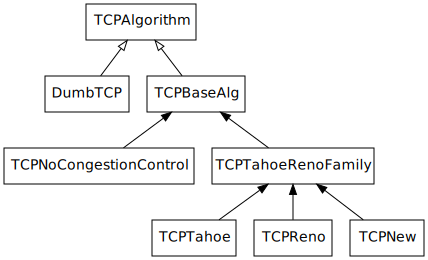
\includegraphics{figures/tcp_algorithms}

The concrete TCP algorithm class to use can be chosen per connection (in OPEN)
or in a module parameter.

\subsection{DumbTCP}

A very-very basic \cppclass{TCPAlgorithm} implementation, with hardcoded
retransmission timeout (2 seconds) and no other sophistication. It can be
used to demonstrate what happened if there was no adaptive
timeout calculation, delayed acks, silly window avoidance,
congestion control, etc. Because this algorithm does not
send duplicate ACKs when receives out-of-order segments,
it does not work well together with other algorithms.

\subsection{TCPBaseAlg}

The \cppclass{TCPBaseAlg} is the base class of the INET implementation
of Tahoe, Reno and New Reno. It implements basic TCP
algorithms for adaptive retransmissions, persistence timers,
delayed ACKs, Nagle's algorithm, Increased Initial Window
-- EXCLUDING congestion control. Congestion control
is implemented in subclasses.

\subsubsection*{Delayed ACK}

When the \fpar{delayedAcksEnabled} parameter is set to \fkeyword{true},
\cppclass{TCPBaseAlg} applies a 200ms delay before sending ACKs.

\subsubsection*{Nagle's algorithm}

When the \fpar{nagleEnabled} parameter is \fkeyword{true}, then
the algorithm does not send small segments if there is outstanding
data. See also \ref{subsec:trans_policies}.

\subsubsection*{Persistence Timer}

The algorithm implements \emph{Persistence Timer} (see \ref{subsec:flow_control}).
When a zero-sized window is received it starts the timer with 5s timeout.
If the timer expires before the window is increased, a 1-byte probe is
sent. Further probes are sent after 5, 6, 12, 24, 48, 60, 60, 60, ...
seconds until the window becomes positive.

\subsubsection*{Initial Congestion Window}

Congestion window is set to 1 SMSS when the connection is established.
If the \fpar{increasedIWEnabled} parameter is true, then the initial
window is increased to 4380 bytes, but at least 2 SMSS and at most 4 SMSS.
The congestion window is not updated afterwards; subclasses can
add congestion control by redefining virtual methods of the
\cppclass{TCPBaseAlg} class.

\subsubsection*{Duplicate ACKs}

The algorithm sends a duplicate ACK when an out-of-order
segment is received or when the incoming segment fills in all
or part of a gap in the sequence space.

\subsubsection*{RTO calculation}

Retransmission timeout ($RTO$) is calculated according to
Jacobson algorithm (with $\alpha=7/8$), and Karn's modification is also applied.
The initial value of the $RTO$ is 3s, its minimum is 1s,
maximum is 240s (2 MSL).

% FIXME according to RFC1222, MIN_REXMIT_TIMEOUT should be a fraction of second
%       to accomodate high speed LANs. In the linux kernel (net/tcp.h)
%       TCP_RTO_MIN is HZ/5 = 200ms. Consider 0ms lower bound.

\subsection{TCPNoCongestion}

TCP with no congestion control (i.e. congestion window kept very large).
Can be used to demonstrate effect of lack of congestion control.

% FIXME 65536 is not 'very large' nowadays, with window scaling
%       the receive window can be as large as 2^30 bytes.
%       Consequently the initial ssthresh is too small for Tahoe/Reno/NewReno,
%       Slow Start is stopped too early first time.

\subsection{TCPTahoe}

The \cppclass{TCPTahoe} algorithm class extends \cppclass{TCPBaseAlg}
with \emph{Slow Start}, \emph{Congestion Avoidance} and
\emph{Fast Retransmit} congestion control algorithms.
This algorithm initiates a \emph{Slow Start} when a packet
loss is detected.

\subsubsection*{Slow Start}

The congestion window is initially set to 1 SMSS or in case of
\fpar{increasedIWEnabled} is \fkeyword{true} to 4380 bytes
(but no less than 2 SMSS and no more than 4 SMSS). The window
is increased on each incoming ACK by 1 SMSS, so it is approximately
doubled in each RTT.

\subsubsection*{Congestion Avoidance}

When the congestion window exceeded $ssthresh$, the window
is increased by $SMSS^2/cwnd$ on each incoming ACK event, so
it is approximately increased by 1 SMSS per RTT.

\subsubsection*{Fast Retransmit}

When the 3rd duplicate ACK received, a packet loss is detected
and the packet is retransmitted immediately. Simultanously
the $ssthresh$ variable is set to half of the $cwnd$ (but at least 2 SMSS)
and $cwnd$ is set to 1 SMSS, so it enters slow start again.

Retransmission timeouts are handled the same way:
$ssthresh$ will be $cwnd/2$, $cwnd$ will be 1 SMSS.

\subsection{TCPReno}

The \cppclass{TCPReno} algorithm extends the behaviour \cppclass{TCPTahoe}
with \emph{Fast Recovery}. This algorithm can also use the information
transmitted in SACK options, which enables a much more accurate
congestion control.

\subsubsection*{Fast Recovery}

When a packet loss is detected by receiveing 3 duplicate ACKs,
$ssthresh$ set to half of the current window as in Tahoe. However
$cwnd$ is set to $ssthresh + 3*SMSS$ so it remains in congestion
avoidance mode. Then it will send one new segment for each incoming
duplicate ACK trying to keep the pipe full of data. This requires
the congestion window to be inflated on each incoming duplicate
ACK; it will be deflated to $ssthresh$ when new data gets
acknowledged.

However a hard packet loss (i.e. RTO events) cause a
slow start by setting $cwnd$ to 1 SMSS.

\subsubsection*{SACK congestion control}

This algorithm can be used with the SACK extension.
Set the \fpar{sackSupport} parameter to \fkeyword{true} to
enable sending and receiving \emph{SACK} options.

\subsection{TCPNewReno}

This class implements the TCP variant known as New Reno.
New Reno recovers more efficiently from multiple packet losses within one RTT
than Reno does.

It does not exit fast-recovery phase until all data which was out-standing
at the time it entered fast-recovery is acknowledged. Thus avoids
reducing the $cwnd$ multiple times.

\section{TCP socket}

%The \cppclass{TCPSocket} C++ class is provided to simplify managing TCP connections
%from applications. \cppclass{TCPSocket} handles the job of assembling and sending
%command messages (OPEN, CLOSE, etc) to \nedtype{TCP}, and it also simplifies
%the task of dealing with packets and notification messages coming from \nedtype{TCP}.

\cppclass{TCPSocket} is a convenience class, to make it easier to manage TCP connections
from your application models. You'd have one (or more) \cppclass{TCPSocket} object(s)
in your application simple module class, and call its member functions
(bind(), listen(), connect(), etc.) to open, close or abort a TCP connection.

TCPSocket chooses and remembers the connId for you, assembles and sends command
packets (such as OPEN\_ACTIVE, OPEN\_PASSIVE, CLOSE, ABORT, etc.) to TCP,
and can also help you deal with packets and notification messages arriving
from TCP.

A session which opens a connection from local port 1000 to 10.0.0.2:2000,
sends 16K of data and closes the connection may be as simple as this
(the code can be placed in your \ffunc{handleMessage()} or
\ffunc{activity()}):

\begin{cpp}
TCPSocket socket;
socket.connect(L3AddressResolver().resolve("10.0.0.2"), 2000);

msg = new cMessage("data1");
msg->setByteLength(16*1024);  16K
socket.send(msg);

socket.close();
\end{cpp}

% FIXME missing setOutputGate() call

Dealing with packets and notification messages coming from TCP is somewhat
more cumbersome. Basically you have two choices: you either process those
messages yourself, or let TCPSocket do part of the job. For the latter,
you give TCPSocket a callback object on which it'll invoke the appropriate
member functions: \ffunc{socketEstablished()}, \ffunc{socketDataArrived()},
\ffunc{socketFailure()}, \ffunc{socketPeerClosed()},
etc (these are methods of \cppclass{TCPSocket::CallbackInterface}).,
The callback object can be your simple module class too.

This code skeleton example shows how to set up a TCPSocket to use the module
itself as callback object:

\begin{cpp}
class MyModule : public cSimpleModule, public TCPSocket::CallbackInterface
{
    TCPSocket socket;
    virtual void socketDataArrived(int connId, void *yourPtr,
                                   cPacket *msg, bool urgent);
    virtual void socketFailure(int connId, void *yourPtr, int code);
    ...
};

void MyModule::initialize() {
    socket.setCallbackObject(this,NULL);
}

void MyModule::handleMessage(cMessage *msg) {
    if (socket.belongsToSocket(msg))
        socket.processMessage(msg); dispatch to socketXXXX() methods
    else
        ...
}

void MyModule::socketDataArrived(int, void *, cPacket *msg, bool) {
    ev << "Received TCP data, " << msg->getByteLength() << " bytes\\n";
    delete msg;
}

void MyModule::socketFailure(int, void *, int code) {
    if (code==TCP_I_CONNECTION_RESET)
        ev << "Connection reset!\\n";
    else if (code==TCP_I_CONNECTION_REFUSED)
        ev << "Connection refused!\\n";
    else if (code==TCP_I_TIMEOUT)
        ev << "Connection timed out!\\n";
}
\end{cpp}

If you need to manage a large number of sockets (e.g. in a server
application which handles multiple incoming connections), the
\cppclass{TCPSocketMap} class may be useful. The following code
fragment to handle incoming connections is from the LDP module:

\begin{cpp}
TCPSocket *socket = socketMap.findSocketFor(msg);
if (!socket)
{
    not yet in socketMap, must be new incoming connection: add to socketMap
    socket = new TCPSocket(msg);
    socket->setOutputGate(gate("tcpOut"));
    socket->setCallbackObject(this, NULL);
    socketMap.addSocket(socket);
}
dispatch to socketEstablished(), socketDataArrived(), socketPeerClosed()
or socketFailure()
socket->processMessage(msg);
\end{cpp}

\section{Other TCP implementations}
\label{sec:other_tcp}

INET contains two other implementation of the TCP protocol:
\nedtype{TCP\_lwIP} and \nedtype{TCP\_NSC}.
All TCP modules implements the \nedtype{ITCP} interface and
communicate with the application and the IP layer through the
same interface. Therefore they can be interchanged and can
operate with each other. See \ffilename{examples/inet/tcpclientserver/omnetpp.ini}
how to parametrize \nedtype{StandardHost}s to use the different
implementations.

\subsection{TCP LWIP}

lwIP is a light-weight implementation of the TCP/IP protocol suite
that was originally written by Adam Dunkels of the Swedish Institute of
Computer Science. The current development homepage is
\url{http://savannah.nongnu.org/projects/lwip/}.

The implementation targets embedded devices: it has
very limited resource usage (it works ``with tens of kilobytes of RAM and
around 40 kilobytes of ROM'') and does not require an underlying OS.

The \nedtype{TCP\_lwIP} simple module is based on the 1.3.2 version of
the lwIP sources.

Features:

\begin{compactitem}
\item delayed ACK
\item Nagle's algorithm
\item round trip time estimation
\item adaptive retransmission timeout
\item SWS avoidance
\item slow start threshold
\item fast retransmit
\item fast recovery
\item persist timer
\item keep-alive timer
\end{compactitem}

\subsubsection*{Limitations}

\begin{itemize}
  \item only MSS and TS TCP options are supported. The TS option is turned off
        by default, but can be enabled by defining LWIP\_TCP\_TIMESTAMPS to 1
        in \ffilename{lwipopts.h}.
  \item \fvar{fork} must be \fkeyword{true} in the passive open command
  \item The status request command (TCP\_C\_STATUS) only reports the
          local and remote addresses/ports of the connection and
          the MSS, SND.NXT, SND.WND, SND.WL1, SND.WL2, RCV.NXT, RCV.WND variables.
\end{itemize}

% lwIP license file missing from INET source
% FIXME TCP_lwIP uses only connId to identify the connection instead of (connId,appGateIndex)
% FIXME status command returns message kind TCP_C_STATUS instead of TCP_I_STATUS

\subsubsection*{Statistics}

The \nedtype{TCP\_lwIP} module generates the following vector files:

\begin{itemize}
  \item \ttt{send window}: value of the $SND.WND$ variable
  \item \ttt{sent seq}: \emph{Sequence Number} of the sent segment
  \item \ttt{sent ack}: \emph{Acknowledgment Number } of the sent segment
  \item \ttt{receive window}: value of the $RCV.WND$ variable
  \item \ttt{rcvd seq}: \emph{Sequence Number} of the received segment
  \item \ttt{rcvd acq}: \emph{Acknowledgment Number} of the received segment
\end{itemize}

% FIXME the following vectors are created, but not used (copy paste?):
%       'sent sacks', 'advertised window', 'rcvd sacks', 'unacked bytes',
%       'rcvd dupAcks', 'pipe', 'rcvd oooseg', 'rcvd sackedBytes',
%       'tcpRcvQueueBytes', 'tcpRcvQueueDrops'
The creation of these vectors can be disabled by setting the \fpar{recordStats}
parameter to \fkeyword{false}.


\subsection{TCP NSC}

Network Simulation Cradle (NSC) is a tool that allow real-world TCP/IP network stacks
to be used in simulated networks. The NSC project is created by Sam Jansen
and available on \url{http://research.wand.net.nz/software/nsc.php}. NSC currently
contains Linux, FreeBSD, OpenBSD and lwIP network stacks, altough on 64-bit
systems only Linux implementations can be built.

To use the \nedtype{TCP\_NSC} module you should download the
\ffilename{nsc-0.5.2.tar.bz2} package and follow the instructions
in the \ffilename{<inet\_root>/3rdparty/README} file to build it.

\begin{warning}
Before generating the INET module, check that the \emph{opp\_makemake} call
in the make file (\ffilename{<inet\_root>/Makefile}) includes the
\emph{-DWITH\_TCP\_NSC} argument. Without this option the \nedtype{TCP\_NSC}
module is not built. If you build the INET library from the IDE, it is enough
to enable the \emph{TCP (NSC)} project feature.
\end{warning}

\subsubsection*{Parameters}

The \nedtype{TCP\_NSC} module has the following parameters:

\begin{itemize}
  \item \fpar{stackName}: the name of the TCP implementation to be used.
  Possible values are: \ttt{liblinux2.6.10.so}, \ttt{liblinux2.6.18.so},
  \ttt{liblinux2.6.26.so}, \ttt{libopenbsd3.5.so}, \ttt{libfreebsd5.3.so} and
  \ttt{liblwip.so}. (On the 64 bit systems, the \ttt{liblinux2.6.26.so} and
  \ttt{liblinux2.6.16.so} are available only).

  \item \fpar{stackBufferSize}: the size of the receive and send buffer of
  one connection for selected TCP implementation.
  The NSC sets the \fvar{wmem\_max}, \fvar{rmem\_max}, \fvar{tcp\_rmem}, \fvar{tcp\_wmem}
  parameters to this value on linux TCP implementations. For details, you can see
  the NSC documentation.
\end{itemize}

\subsubsection*{Statistics}

The \nedtype{TCP\_NSC} module collects the following vectors:

\begin{itemize}
  \item \ttt{sent seq} \emph{Sequence Number} of the sent TCP segment
  \item \ttt{sent ack} \emph{Acknowledgment Number} of the sent TCP segment
  \item \ttt{rcvd seq} \emph{Sequence Number} of the received TCP segment
  \item \ttt{rcvd ack} \emph{Acknowledgement Number} of the received TCP segment
\end{itemize}

\subsubsection*{Limitations}

\begin{itemize}
\item Because the kernel code is not reentrant, NSC creates a record containing
the global variables of the stack implementation. By default there is room
for 50 instance in this table, so you can not create more then 50 instance
of \nedtype{TCP\_NSC}. You can increase the \fvar{NUM\_STACKS} constant
in \ffilename{num\_stacks.h} and recompile NSC to overcome this limitation.

\item The \nedtype{TCP\_NSC} module does not supprt TCP\_TRANSFER\_OBJECT
data transfer mode.

\item The MTU of the network stack fixed to 1500, therefore MSS is 1460.

\item TCP\_C\_STATUS command reports only local/remote addresses/ports and
      current window of the connection.

\end{itemize}

% local address: 1.0.0.253, gateway address: 1.0.0.254, remote addresses: 2.0.0.1, 2.0.0.2, ...

% FIXME connections are identified by connId, not by (appGateIndex,connId) as in TCP module.
% FIXME TCP_NSC_Connection::getSocket() and TCP_NSC_Connection::do_checkedclose() are declared but not implemented

\section{TCP applications}

This sections describes the applications using the TCP protocol.
Each application must implement the \nedtype{ITCPApp} module interface
to ease configuring the \nedtype{StandardHost} module.

The applications described here are all contained by the
\nedtype{inet.applications.tcpapp} package. These applications use
\msgtype{GenericAppMsg} objects to represent the data sent between the client
and server. The client message contains the expected reply length, the
processing delay, and a flag indicating that the connection should be closed
after sending the reply. This way intelligence (behaviour specific to the
modelled application, e.g. HTTP, SMB, database protocol) needs only to be
present in the client, and the server model can be kept simple and dumb.


\subsection{TCPBasicClientApp}

Client for a generic request-response style protocol over TCP.
May be used as a rough model of HTTP or FTP users.

The model communicates with the server in sessions. During a session,
the client opens a single TCP connection to the server, sends several
requests (always waiting for the complete reply to arrive before
sending a new request), and closes the connection.

The server app should be \nedtype{TCPGenericSrvApp}; the model sends
\msgtype{GenericAppMsg} messages.

Example settings:

\begin{description}
\item[FTP] \quad \\

\begin{inifile}
numRequestsPerSession = exponential(3)
requestLength = truncnormal(20,5)
replyLength = exponential(1000000)
\end{inifile}

\item[HTTP] \quad \\

\begin{inifile}
numRequestsPerSession = 1 # HTTP 1.0
numRequestsPerSession = exponential(5)  # HTTP 1.1, with keepalive
requestLength = truncnormal(350,20)
replyLength = exponential(2000)
\end{inifile}

\end{description}

Note that since most web pages contain images and may contain frames,
applets etc, possibly from various servers, and browsers usually download
these items in parallel to the main HTML document, this module cannot
serve as a realistic web client.

Also, with HTTP 1.0 it is the server that closes the connection after
sending the response, while in this model it is the client.

\subsection{TCPSinkApp}

Accepts any number of incoming TCP connections, and discards whatever
arrives on them.

The module parameter \fpar{dataTransferMode} should be set the transfer mode in TCP layer.
Its possible values (``bytecount'', ``object'', ``bytestream'') are described in ...

\subsection{TCPGenericSrvApp}

Generic server application for modelling TCP-based request-reply style
protocols or applications.

Requires message object preserving sendQueue/receiveQueue classes
to be used with \nedtype{TCP} (that is, TCPMsgBasedSendQueue and TCPMsgBasedRcvQueue;
TCPVirtualBytesSendQueue/RcvQueue are not good).

The module accepts any number of incoming TCP connections, and expects
to receive messages of class \msgtype{GenericAppMsg} on them. A message should
contain how large the reply should be (number of bytes). \nedtype{TCPGenericSrvApp}
will just change the length of the received message accordingly, and send
back the same message object. The reply can be delayed by a constant time
(replyDelay parameter).

\subsection{TCPEchoApp}

The \nedtype{TCPEchoApp} application accepts any number of incoming TCP
connections, and sends back the messages that arrive on them, The lengths of the
messages are multiplied by \fpar{echoFactor} before sending them back (echoFactor=1
will result in sending back the same message unmodified.) The reply can also be
delayed by a constant time (\fpar{echoDelay} parameter).

When \nedtype{TCPEchoApp} receives data packets from TCP (and such, when they can be
echoed) depends on the dataTransferMode setting.
With "bytecount" and "bytestream", TCP passes up data to us
as soon as a segment arrives, so it can be echoed immediately.
With "object" mode, our local TCP reproduces the same
messages that the sender app passed down to its TCP -- so if the sender
app sent a single 100 MB message, it will be echoed only when all
100 megabytes have arrived.

\subsection{TCPSessionApp}

Single-connection TCP application: it opens a connection, sends
the given number of bytes, and closes. Sending may be one-off,
or may be controlled by a "script" which is a series of
(time, number of bytes) pairs. May act either as client or as server,
and works with TCPVirtualBytesSendQueue/RcvQueue as sendQueue/receiveQueue
setting for ~TCP.
Compatible with both IPv4 (~IPv4) and ~IPv6.

\subsubsection*{Opening the connection}

Regarding the type of opening the connection, the application may
be either a client or a server. When active=false, the application
will listen on the given local localPort, and wait for an incoming connection.
When active=true, the application will bind to given local localAddress:localPort,
and connect to the connectAddress:connectPort. To use an ephemeral port
as local port, set the localPort parameter to -1.

Even when in server mode (active=false), the application will only
serve one incoming connection. Further connect attempts will be
refused by TCP (it will send RST) for lack of LISTENing connections.

The time of opening the connection is in the tOpen parameter.

\subsubsection*{Sending data}

Regardless of the type of OPEN, the application can be made to send
data. One way of specifying sending is via the tSend, sendBytes
parameters, the other way is sendScript. With the former, sendBytes
bytes will be sent at tSend. With sendScript, the format is
"<time> <numBytes>;<time> <numBytes>;..."

\subsubsection*{Closing the connection}

The application will issue a TCP CLOSE at time tClose. If tClose=-1, no
CLOSE will be issued.



\subsection{TelnetApp}

Models Telnet sessions with a specific user behaviour.
The server app should be \nedtype{TCPGenericSrvApp}.

In this model the client repeats the following activity
between \fpar{startTime} and \fpar{stopTime}:

\begin{enumerate}
\item opens a telnet connection
\item sends \fpar{numCommands} commands. The command is \fpar{commandLength} bytes
      long. The command is transmitted as entered by the user character by character,
      there is \fpar{keyPressDelay} time between the characters. The server echoes
      each character. When the last character of the command is sent (new line),
      the server responds with a \fpar{commandOutputLength} bytes long message.
      The user waits \fpar{thinkTime} interval between the commands.
\item closes the connection and waits \fpar{idleInterval} seconds
\item if the connection is broken it is noticed after \fpar{reconnectInterval}
      and the connection is reopened
\end{enumerate}

Each parameter in the above description is ``volatile'', so you can
use distributions to emulate random behaviour.

Additional parameters:
addresses,ports
dataTransferMode

\begin{note}
This module emulates a very specific user behaviour, and as such,
it should be viewed as an example rather than a generic Telnet model.
If you want to model realistic Telnet traffic, you are encouraged
to gather statistics from packet traces on a real network, and
write your model accordingly.
\end{note}

\subsection{TCPSrvHostApp}

This module hosts TCP-based server applications. It dynamically creates
and launches a new "thread" object for each incoming connection.

Server threads should be subclassed from the \cppclass{TCPServerThreadBase}
C++ class, registered in the C++ code using the Register\_Class() macro,
and the class name should be specified in the serverThreadClass
parameter of \nedtype{TCPSrvHostApp}. The thread object will receive events
via a callback interface (methods like established(), dataArrived(),
peerClosed(), timerExpired()), and can send packets via TCPSocket's send()
method.

Example server thread class: \cppclass{TCPGenericSrvThread}.

\begin{important}
Before you try to use this module, make sure you actually need it!
In most cases, \nedtype{TCPGenericSrvApp} and \msgtype{GenericAppMsg} will be completely
enough, and they are a lot easier to handle. You'll want to subclass your
client from \cppclass{TCPGenericCliAppBase} then; check \nedtype{TelnetApp} and
\nedtype{TCPBasicClientApp} for examples.
\end{important}

%%% Local Variables:
%%% mode: latex
%%% TeX-master: "usman"
%%% End:


\cleardoublepage

\ifdraft TODO
\chapter{The SCTP Model}
\label{cha:sctp}


\section{Overview}

Blah blah blah


%%% Local Variables:
%%% mode: latex
%%% TeX-master: "usman"
%%% End:


\cleardoublepage
\fi

\ifdraft TODO
\chapter{Internet Routing}
\label{cha:routing}

\section{Overview}
\label{sec:routing:overview}

INET Framework has models for several internet routing protocols, including
RIP, OSPF and BGP.

The easiest way to add routing to a network is to use the \nedtype{Router}
NED type for routers. \nedtype{Router} contains a conditional instance
for each of the above protocols. These submodules can be enabled by
setting the \ttt{hasRip}, \ttt{hasOspf} and/or \ttt{hasBgp} parameters to
\ttt{true}.

Example:

\begin{inifile}
**.hasRip = true
\end{inifile}

There are also NED types called \nedtype{RipRouter}, \nedtype{OspfRouter},
\nedtype{BgpRouter}, which are all \nedtype{Router}'s with appropriate
routing protocol enabled.

\section{RIP}
\label{sec:routing:rip}

RIP (Routing Information Protocol) is a distance-vector routing protocol which
employs the hop count as a routing metric. RIP prevents routing loops by
implementing a limit on the number of hops allowed in a path from source to
destination.  RIP uses the \textit{split horizon with poison reverse} technique
to work around the ``count-to-infinity'' problem.

The \nedtype{Rip} module implements distance vector routing as specified in RFC
2453 (RIPv2) and RFC 2080 (RIPng). The behavior can be selected by setting the
\fpar{mode} parameter to either \ttt{"RIPv2"} or \ttt{"RIPng"}. Protocol
configuration such as link metrics and per-interface operation mode (such as
whether RIP is enabled on the interface, and whether to use split horizon)
can be specified in XML using the \ttt{ripConfig} parameter.

The following example configures a \nedtype{Router} module to use RIPv2:

\begin{inifile}
**.hasRip = true
**.mode = "RIPv2"
**.ripConfig = xmldoc("RIPConfig.xml")
\end{inifile}

The configuration file specifies the per interface parameters.
Each \ttt{<interface>} element configures one or more interfaces;
the \ttt{hosts}, \ttt{names}, \ttt{towards}, \ttt{among} attributes
select the configured interfaces (in a similar way as with
\nedtype{Ipv4NetworkConfigurator} \ref{cha:network-autoconfiguration}).

Additional attributes:

\begin{itemize}
  \item \ttt{metric}: metric assigned to the link, default value is 1.
        This value is added to the metric of a learned route,
        received on this interface. It must be an integer in
        the [1,15] interval.
  \item \ttt{mode}: mode of the interface.
\end{itemize}

The mode attribute can be one of the following:

\begin{itemize}
  \item \ttt{'NoRIP'}: no RIP messages are sent or received on this interface.
  \item \ttt{'NoSplitHorizon'}: no split horizon filtering; send all routes to
        neighbors.
  \item \ttt{'SplitHorizon'}: do not sent routes whose next hop is the neighbor.
  \item \ttt{'SplitHorizonPoisenedReverse'} (default): if the next hop is the neighbor, then
  set the metric of the route to infinity.
\end{itemize}

The following example sets the link metric between router
\ttt{R1} and \ttt{RB} to 2, while all other links will have a metric of 1.

\begin{XML}
<RIPConfig>
  <interface among="R1 RB" metric="2"/>
  <interface among="R? R?" metric="1"/>
</RIPConfig>
\end{XML}

\section{OSPF}
\label{sec:routing:ospf}

OSPF (Open Shortest Path First) is a routing protocol for IP networks.
It uses a link state routing (LSR) algorithm and falls into the group
of interior gateway protocols (IGPs), operating within a single
autonomous system (AS).

\nedtype{OspfRouter} is a \nedtype{Router} with the OSPF protocol enabled.

The \nedtype{Ospf} module implements OSPF protocol version 2. Areas and routers
can be configured using an XML file specified by the \ttt{ospfConfig} parameter.
Various parameters for the network interfaces can be specified also in the XML
file or as a parameter of the \nedtype{Ospf} module.

\begin{inifile}
**.ospf.ospfConfig = xmldoc("ASConfig.xml")
**.ospf.helloInterval = 12s
**.ospf.retransmissionInterval = 6s
\end{inifile}

The \ttt{<OSPFASConfig>} root element may contain \ttt{<Area>} and \ttt{<Router>}
elements with various attributes specifying the parameters for the network
interfaces. Most importantly \ttt{<Area>} contains \ttt{<AddressRange>} elements
enumerating the network addresses that should be advertized by the protocol.
Also \ttt{<Router>} elements may contain data for configuring various pont-to-point
or broadcast interfaces.

\begin{XML}
<?xml version="1.0"?>
<OSPFASConfig xmlns:xsi="http://www.w3.org/2001/XMLSchema-instance" xsi:schemaLocation="OSPF.xsd">
  <!-- Areas -->
  <Area id="0.0.0.0">
    <AddressRange address="H1" mask="H1" status="Advertise" />
    <AddressRange address="H2" mask="H2" status="Advertise" />
    <AddressRange address="R1>R2" mask="R1>R2" status="Advertise" />
    <AddressRange address="R2>R1" mask="R2>R1" status="Advertise" />
  </Area>
  <!-- Routers -->
  <Router name="R1" RFC1583Compatible="true">
    <BroadcastInterface ifName="eth0" areaID="0.0.0.0" interfaceOutputCost="1" routerPriority="1" />
    <PointToPointInterface ifName="eth1" areaID="0.0.0.0" interfaceOutputCost="2" />
  </Router>
  <Router name="R2" RFC1583Compatible="true">
    <PointToPointInterface ifName="eth0" areaID="0.0.0.0" interfaceOutputCost="2" />
    <BroadcastInterface ifName="eth1" areaID="0.0.0.0" interfaceOutputCost="1" routerPriority="2" />
  </Router>
</OSPFASConfig>
\end{XML}

\section{BGP}
\label{sec:routing:bgp}

BGP (Border Gateway Protocol) is a standardized exterior gateway protocol
designed to exchange routing and reachability information among
autonomous systems (AS) on the Internet.

\nedtype{BgpRouter} is a \nedtype{Router} with the BGP protocol enabled.

The \nedtype{Bgp} module implements BGP Version 4. The model implements
RFC 4271, with some limitations. Autonomous Systems and rules can be
configured in an XML file that can be specified in the \ttt{bgpConfig}
parameter.

\begin{inifile}
**.bgpConfig = xmldoc("BGPConfig.xml")
\end{inifile}

The configuration file may contain \ttt{<TimerParams>}, \ttt{<AS>} and
\ttt{Session} elements at the top level.

\begin{itemize}
  \item \ttt{<TimerParams>}: allows specifying various timing parameters
  for the routers.
  \item \ttt{<AS>}: defines Autonomous Systems, routers and rules to be applied.
  \item \ttt{<Session>}: specifies open sessions between edge routers. It must
  contain exactly two \ttt{<Router exterAddr="x.x.x.x"/>} elements.
\end{itemize}

\begin{XML}
<BGPConfig xmlns:xsi="http://www.w3.org/2001/XMLSchema-instance"
  xsi:schemaLocation="BGP.xsd">

  <TimerParams>
    <connectRetryTime> 120 </connectRetryTime>
    <holdTime> 180 </holdTime>
    <keepAliveTime> 60 </keepAliveTime>
    <startDelay> 15 </startDelay>
  </TimerParams>

  <AS id="60111">
    <Router interAddr="172.1.10.255"/> <!--Router A1-->
    <Router interAddr="172.1.20.255"/> <!--Router A2-->
  </AS>

  <AS id="60222">
    <Router interAddr="172.10.4.255"/> <!--Router B-->
  </AS>

  <AS id="60333">
    <Router interAddr="172.13.1.255"/> <!--Router C1-->
    <Router interAddr="172.13.2.255"/> <!--Router C2-->
    <Router interAddr="172.13.3.255"/> <!--Router C3-->
    <Router interAddr="172.13.4.255"/> <!--Router C4-->
    <DenyRouteOUT Address="172.10.8.0" Netmask="255.255.255.0"/>
    <DenyASOUT> 60111 </DenyASOUT>
  </AS>

  <Session id="1">
    <Router exterAddr="10.10.10.1" > </Router> <!--Router A1-->
    <Router exterAddr="10.10.10.2" > </Router> <!--Router C1-->
  </Session>

  <Session id="2">
    <Router exterAddr="10.10.20.1" > </Router> <!--Router A2-->
    <Router exterAddr="10.10.20.2" > </Router> <!--Router B-->
  </Session>

  <Session id="3">
    <Router exterAddr="10.10.30.1" > </Router> <!--Router B-->
    <Router exterAddr="10.10.30.2" > </Router> <!--Router C2-->
  </Session>
</BGPConfig>
\end{XML}

Inside \ttt{<AS>} elements various rules can be sepecified:

\begin{itemize}
  \item DenyRoute: deny route in IN and OUT traffic (\ttt{Address} and
        \ttt{Netmask} attributes must be specified.)
  \item DenyRouteIN : deny route in IN traffic (\ttt{Address} and
        \ttt{Netmask} attributes must be specified.)
  \item DenyRouteOUT: deny route in OUT traffic (\ttt{Address} and
        \ttt{Netmask} attributes must be specified.)
  \item DenyAS: deny routes learned by AS in IN  and OUT traffic (AS id must be
        specified as the body of the element.)
  \item DenyASIN : deny routes learned by AS in IN traffic (AS id must be
        specified as the body of the element.)
  \item DenyASOUT: deny routes learned by AS in OUT traffic (AS id must be
        specified as the body of the element.)
\end{itemize}

%%% Local Variables:
%%% mode: latex
%%% TeX-master: "usman"
%%% End:


\cleardoublepage
\fi

\chapter{Differentiated Services}
\label{cha:diffserv}


\section{Overview}

In the early days of the Internet, only best effort service was defined.
The Internet delivers individually each packet, and delivery time is not
guaranteed, moreover packets may even be dropped due to congestion at
the routers of the network. It was assumed that transport protocols,
and applications can overcome these deficiencies. This worked until
FTP and email was the main applications of the Internet, but the newer
applications such as Internet telephony and video conferencing cannot
tolerate delay jitter and loss of data.

% TypeOfService field

The first attempt to add QoS capabilities to the IP routing was
Integrated Services. Integrated services provide resource assurance
through resource reservation for individual application flows.
An application flow is identified by the source and destination
addresses and ports and the protocol id. Before data packets are
sent the necessary resources must be allocated along the path
from the source to the destination. At the hops from the source
to the destination each router must examine the packets, and decide
if it belongs to a reserved application flow. This could cause a
memory and processing demand in the routers.
Other drawback is that
the reservation must be periodically refreshed, so there is an overhead
during the data transmission too.

Differentiated Services is a more scalable approach to offer a better than
best-effort service. Differentiated Services do not require resource reservation
setup. Instead of making per-flow reservations, Differentiated
Services divides the traffic into a small number of \emph{forwarding classes}.
The forwarding class is directly encoded into the packet header. After packets are
marked with their forwarding classes at the edge of the network, the interior nodes
of the network can use this information to differentiate the treatment of packets.
The forwarding classes may indicate drop priority and resource priority. For example,
when a link is congested, the network will drop packets with the highest drop priority
first.

In the Differentiated Service architecture, the network is partitioned into
DiffServ domains. Within each domain the resources of the domain are allocated
to forwarding classes, taking into account the available resources and the
traffic flows. There are \emph{service level agggreements} (SLA) between the users
and service providers, and between the domains that describe the mapping of
packets to forwarding classes and the allowed traffic profile for each class.
The routers at the edge of the network are responsible for marking the packets
and protect the domain from misbehaving traffic sources. Nonconforming traffic
may be dropped, delayed, or marked with a different forwarding class.


\subsection{Implemented Standards}

The implementation follows these RFCs below:

\begin{itemize}
  \item RFC 2474: Definition of the Differentiated Services Field (DS Field) in the IPv4 and IPv6 Headers
  \item RFC 2475: An Architecture for Differentiated Services
  \item RFC 2597: Assured Forwarding PHB Group
  \item RFC 2697: A Single Rate Three Color Marker
  \item RFC 2698: A Two Rate Three Color Marker
  \item RFC 3246: An Expedited Forwarding PHB (Per-Hop Behavior)
  \item RFC 3290: An Informal Management Model for Diffserv Routers
\end{itemize}

\section{Architecture of NICs}

Network Interface Card (NIC) modules, such as \nedtype{PppInterface} and
\nedtype{EthernetInterface}, may contain traffic conditioners in
their input and output data path. Traffic conditioners have one input
and one output gate as defined in the \nedtype{ITrafficConditioner}
interface. They can transform the incoming traffic by dropping or
delaying packets. They can also set the DSCP field of the packet,
or mark them other way, for differentiated handling in the queues.

The NICs may also contain an external queue component. If the \fpar{queueType}
parameter is set, it must contain a module type implementing the \nedtype{IOutputQueue}
module interface. If it is not specified, then \nedtype{Ppp} and \nedtype{EtherMac}
use an internal drop tail queue to buffer the packets until the line is busy.

\subsection{Traffic Conditioners}

Traffic conditioners have one input
and one output gate as defined in the \nedtype{ITrafficConditioner}
interface. They can transform the incoming traffic by dropping or
delaying packets. They can also set the DSCP field of the packet,
or mark them other way, for differentiated handling in the queues.

Traffic conditioners perform the following actions:
\begin{itemize}
 \item classify the incoming packets
 \item meter the traffic in each class
 \item marks/drops packets depending on the result of metering
 \item shape the traffic by delaying packets to conform to the
       desired traffic profile
\end{itemize}

INET provides classifier, meter, and marker modules, that can be
composed to build a traffic conditioner as a compound module.

\subsection{Output Queues}

The queue component also has one input and one output gate. These components
must implement a passive queue behaviour: they only deliver a packet,
when the module connected to its output explicitly asks them.
In terms of C++ it means, that the simple module owning the \fgate{out} gate,
or which is connected to the \fgate{out} gate of the compound module,
must implement the \cppclass{IPassiveQueue} interface. The next module
asks a packet by calling the \ffunc{requestPacket()} method of this interface.


\section{Simple modules}

This section describes the primitive elements from which traffic
conditioners and output queues can be built. The next sections
shows some examples, how these queues, schedulers, droppers,
classifiers, meters, markers can be combined.

The type of the components are:
\begin{itemize}
  \item \ttt{queue}: container of packets, accessed as FIFO
  \item \ttt{dropper}: attached to one or more queue, it can
    limit the queue length below some threshold
    by selectively dropping packets
  \item \ttt{scheduler}: decide which packet is transmitted first,
     when more packets are available on their inputs
  \item \ttt{classifier}: classify the received packets
     according to their content (e.g. source/destination,
     address and port, protocol, dscp field of IP datagrams)
     and forward them to the corresponding output gate.
  \item \ttt{meter}: classify the received packets
      according to the temporal characteristic of their
      traffic stream
  \item \ttt{marker}: marks packets by setting their fields
      to control their further processing
\end{itemize}

\subsection{Queues}

When packets arrive at higher rate, than the interface can trasmit,
they are getting queued.


Queue elements store packets until they can be transmitted.
They have one input and one output gate.
Queues may have one or more thresholds associated with them.

 Received packets
are enqueued and stored until the module connected to their
output asks a packet by calling the \ffunc{requestPacket()}
method.

They should be able to notify the module connected to its output
about the arrival of new packets.

\subsubsection{FIFO Queue}

The \nedtype{FifoQueue} module implements a passive
FIFO queue with unlimited buffer space. It can be combined
with algorithmic droppers and schedulers to form an
IOutputQueue compound module.

The C++ class implements the \cppclass{IQueueAccess} and
\cppclass{IPassiveQueue} interfaces.

\subsubsection{DropTailQueue}

The other primitive queue module is \nedtype{DropTailQueue}.
Its capacity can be specified by the \fpar{frameCapacity}
parameter. When the number of stored packet reached the capacity
of the queue, further packets are dropped.
Because this module contains a built-in dropping strategy, it
cannot be combined with algorithmic droppers as \nedtype{FifoQueue}
can be. However its output can be connected to schedulers.

This module implements the \nedtype{IOutputQueue} interface,
so it can be used as the queue component of interface card per se.

\subsection{Droppers}

Algorithmic droppers selectively drop received packets based on some condition.
The condition can be either deterministic (e.g. to bound the queue length),
or probabilistic (e.g. RED queues).

Other kind of droppers are absolute droppers; they drop each received
packet. They can be used to discard excess traffic, i.e. packets whose
arrival rate exceeds the allowed maximum. In INET the \nedtype{Sink}
module can be used as an absolute dropper.

The algorithmic droppers in INET are \nedtype{ThresholdDropper} and
\nedtype{RedDropper}. These modules has multiple input and multiple
output gates. Packets that arrive on gate \fgate{in[i]} are forwarded
to gate \fgate{out[i]} (unless they are dropped). However the queues
attached to the output gates are viewed as a whole, i.e. the queue
length parameter of the dropping algorithm is the sum of the individual
queue lengths. This way we can emulate shared buffers of the queues.
Note, that it is also possible to connect each output to the same
queue module.

\subsubsection{Threshold Dropper}

The \nedtype{ThresholdDropper} module selectively drops packets,
based on the available buffer space of the queues attached to its output.
The buffer space can be specified as the count of packets, or as the size
in bytes.

The module sums the buffer lengths of its outputs
and if enqueuing a packet would exceed the configured
capacities, then the packet will be dropped instead.

By attaching a \nedtype{ThresholdDropper} to the input of a FIFO
queue, you can compose a drop tail queue. Shared buffer
space can be modeled by attaching more FIFO queues
to the output.

\subsubsection*{RED Dropper}

The \nedtype{RedDropper} module implements Random Early Detection
(\cite{Floyd93randomearly}).

It has $n$ input and $n$ output gates (specified by the
\fpar{numGates} parameter). Packets that arrive at the $i^{th}$ input
gate are forwarded to the $i^{th}$ output gate, or dropped.
The output gates must be connected to simple modules implementing
the \nedtype{IQueueAccess} C++ interface (e.g. \nedtype{FifoQueue}).

The module sums the used buffer space of the queues attached
to the output gates. If it is below a minimum threshold,
the packet won't be dropped, if above a maximum threshold,
it will be dropped, if it is between the minimum and
maximum threshold, it will be dropped by a given probability.
This probability determined by a linear function which is
0 at the minth and maxp at maxth.

\begin{center}
\setlength{\unitlength}{1cm}
\begin{picture}(7,4)(-1,-1)
\put(-0.5,0){\vector(1,0){6.5}}
\put(0,-0.5){\vector(0,1){3.5}}
\put(5.8,-0.3){$qlen$}
\put(-0.5,3){$p$}
\put(1,0){\line(3,1){3}}
\put(4,1){\line(0,1){1}}
\put(4,2){\line(1,0){1.5}}
\put(-0.5,1.9){$1$}
%\put(-0.2,2){\line(1,0){0.2}}
\multiput(0,2)(0.4,0){10}{\line(1,0){0.2}}
%\put(-0.2,1){\line(1,0){0.2}}
\multiput(0,1)(0.4,0){10}{\line(1,0){0.2}}
\put(-1,0.9){$p_{max}$}
\multiput(4,0)(0,0.4){3}{\line(0,1){0.2}}
\put(0.9,-0.3){$th_{min}$}
\put(3.9,-0.3){$th_{max}$}
\end{picture}
\end{center}

The queue length can be smoothed by specifying the \fpar{wq}
parameter. The average queue length used in the tests
are computed by the formula:

 $$avg = (1-wq)*avg + wq*qlen$$

The \fpar{minth}, \fpar{maxth}, and \fpar{maxp} parameters
can be specified separately for each input gate, so this module
can be used to implement different packet drop priorities.

\subsection{Schedulers}

Scheduler modules decide which queue can send a packet, when the
interface is ready to transmit one. They have several input gates
and one output gate.

Modules that are connected to the inputs of a scheduler must
implement the \cppclass{IPassiveQueue} C++ interface.
Schedulers also implement \cppclass{IPassiveQueue}, so
they can be cascaded to other schedulers, and can be used
as the output module of \nedtype{IOutputQueue}s.

There are several possible scheduling discipline (first come/first served,
priority, weighted fair, weighted round-robin, deadline-based,
rate-based). INET contains implementation
of priority and weighted round-robin schedulers.

\subsubsection{Priority Scheduler}

The \nedtype{PriorityScheduler} module implements a strict priority
scheduler. Packets that arrived on \fgate{in[0]} has the highest priority,
then packets arrived on \fgate{in[1]}, and so on. If more packets
available when one is requested, then the one with highest priority
is chosen. Packets with lower priority are transmitted only when
there are no packets on the inputs with higher priorities.

\nedtype{PriorityScheduler} must be used with care, because a
large volume of higher packets can starve lower priority packets.
Therefore it is necessary to limit the rate of higher priority
packets to a fraction of the output datarate.

\nedtype{PriorityScheduler} can be used to implement
the \ttt{EF} PHB.

\subsubsection*{Weighted Round Robin Scheduler}

The \nedtype{WrrScheduler} module implements a weighted
round-robin scheduler. The scheduler visits the input gates
in turn and selects the number of packets for transmission
based on their weight.

For example if the module has three input gates, and the weights
are 3, 2, and 1, then packets are transmitted in this order:
\begin{verbatim}
A, A, A, B, B, C, A, A, A, B, B, C, ...
\end{verbatim}
where A packets arrived on \fgate{in[0]}, B packets on \fgate{in[1]},
and C packets on \fgate{in[2]}. If there are no packets in the current
one when a packet is requested, then the next one is chosen that has
enough tokens.

If the size of the packets are equal, then \nedtype{WrrScheduler}
divides the available bandwith according to the weights. In each
case, it allocates the bandwith fairly. Each flow receives a guaranteed
minimum bandwith, which is ensured even if other flows exceed
their share (flow isolation). It is also efficiently uses the
channel, because if some traffic is smaller than its share of
bandwidth, then the rest is allocated to the other flows.

\nedtype{WrrScheduler} can be used to implement the \ttt{AFxy} PHBs.

\subsection{Classifiers}

Classifier modules have one input and many output gates.
They examine the received packets, and forward them to the
appropriate output gate based on the content of some portion
of the packet header. You can read more about classifiers
in RFC 2475 2.3.1 and RFC 3290 4.

The \nedtype{inet.networklayer.diffserv} package contains two
classifiers: \nedtype{MultiFieldClassifier} to classify
the packets at the edge routers of the DiffServ domain, and
\nedtype{BehaviorAggregateClassifier} to classify the packets
at the core routers.


\subsubsection*{Multi-field Classifier}

The \nedtype{MultiFieldClassifier} module can be used to identify
micro-flows in the incoming traffic. The flow is identified
by the source and destination addresses, the protocol id,
and the source and destination ports of the IP packet.

The classifier can be configured by specifying a list of filters.
Each filter can specify a source/destination address mask, protocol,
source/destination port range, and bits of TypeOfService/TrafficClass
field to be matched. They also specify the index of the output gate
matching packet should be forwarded to. The first matching filter
determines the output gate, if there are no matching filters,
then \fgate{defaultOut} is chosen.

The configuration of the module is given as an XML document.
The document element must contain a list of \ttt{<filter>} elements.
The filter element has a mandatory \ttt{@gate} attribute that gives
the index of the gate for packets matching the filter. Other attributes
are optional and specify the condition of matching:
\begin{compactitem}
  \item \ttt{@srcAddress}, \ttt{@srcPrefixLength}: to match the source
    address of the IP
  \item \ttt{@destAddress}, \ttt{@destPrefixLength}:
  \item \ttt{@protocol}: matches the protocol field of the IP packet.
    Its value can be a name (e.g. ``udp'', ``tcp''),
    or the numeric code of the protocol.
  \item \ttt{@tos},{@tosMask}: matches bits of the TypeOfService/TrafficClass
    field of the IP packet.
  \item \ttt{@srcPort}: matches the source port of the TCP or UDP packet.
  \item \ttt{@srcPortMin}, \ttt{@srcPortMax}: matches a range of source ports.
  \item \ttt{@destPort}: matches the destination port of the TCP or UDP packet.
  \item \ttt{@destPortMin}, \ttt{@destPortMax}: matches a range of
     destination ports.
\end{compactitem}

The following example configuration specifies
\begin{compactitem}
  \item to transmit packets received from the 192.168.1.x subnet on gate 0,
  \item to transmit packets addressed to port 5060 on gate 1,
  \item to transmit packets having CS7 in their DSCP field on gate 2,
  \item to transmit other packets on \fgate{defaultGate}.
\end{compactitem}

\begin{verbatim}
<filters>
  <filter srcAddress="192.168.1.0" srcPrefixLength="24" gate="0"/>
  <filter protocol="udp" destPort="5060" gate="1"/>
  <filter tos="0b00111000" tosMask="0x3f" gate="2"/>
</filters>
\end{verbatim}

\subsubsection*{Behavior Aggregate Classifier}

The \nedtype{BehaviorAggregateClassifier} module can be used to read
the DSCP field from the IP datagram, and direct the packet to
the corresponding output gate. The DSCP value is the lower
six bits of the TypeOfService/TrafficClass field. Core routers
usually use this classifier to guide the packet to the appropriate
queue.

DSCP values are enumerated in the \fpar{dscps} parameter.
The first value is for gate \fgate{out[0]}, the second for
\fgate{out[1]}, so on. If the received packet has a DSCP
value not enumerated in the \fpar{dscps} parameter, it will
be forwarded to the \nedtype{defaultOut} gate.

\subsection{Meters}

Meters classify the packets based on the temporal characteristics
of their arrival. The arrival rate of packets is compared to an
allowed traffic profile, and packets are decided to be green
(in-profile) or red (out-of-profile). Some meters apply more than two
conformance level, e.g. in three color meters the partially conforming
packets are classified as yellow.

The allowed traffic profile is usually specified by a token bucket.
In this model, a bucket is filled in with tokens with a specified rate,
until it reaches its maximum capacity. When a packet arrives, the
bucket is examined. If it contains at least as many tokens as the
length of the packet, then that tokens are removed, and the packet
marked as conforming to the traffic profile. If the bucket contains
less tokens than needed, it left unchanged, but the packet marked
as non-conforming.

Meters has two modes: color-blind and color-aware.
In color-blind mode, the color assigned by a previous meter does not
affect the classification of the packet in subsequent meters.
In color-aware mode, the color of the packet can not be changed to a less
conforming color: if a packet is classified as non-conforming by a meter,
it also handled as non-conforming in later meters in the data path.

\begin{important}
Meters take into account the length of the IP packet only, L2 headers are omitted
from the length calculation. If they receive a packet which is not
an IP datagram and does not encapsulate an IP datagram, an error occurs.
\end{important}

\subsubsection*{TokenBucketMeter}

The \nedtype{TokenBucketMeter} module implements a simple token bucket meter.
The module has two output, one for green packets, and one for red packets.
When a packet arrives, the gained tokens are added to the bucket, and
the number of tokens equal to the size of the packet are subtracted.

Packets are classified according to two parameters,
Committed Information Rate ($cir$), Committed Burst Size ($cbs$),
to be either green, or red.

Green traffic is guaranteed to be under $cir*(t_1-t_0)+8*cbs$ in
every $[t_0,t_1]$ interval.

\subsubsection*{SingleRateThreeColorMeter}

The \nedtype{SingleRateThreeColorMeter} module implements a
Single Rate Three Color Meter (RFC 2697).
The module has three output for green, yellow, and red packets.

Packets are classified according to three parameters,
Committed Information Rate ($cir$), Committed Burst Size ($cbs$),
and Excess Burst Size ($ebs$), to be either green, yellow or red.
The green traffic is guaranteed to be under $cir*(t_1-t_0)+8*cbs$,
while the green+yellow traffic to be under $cir*(t_1-t_0)+8*(cbs+ebs)$
in every $[t_0,t_1]$ interval.


\subsubsection*{TwoRateThreeColorMeter}

The \nedtype{TwoRateThreeColorMeter} module implements a
Two Rate Three Color Meter (RFC 2698). The module has three output
gates for the green, yellow, and red packets.

It classifies the packets based on two rates, Peak Information Rate ($pir$)
and Committed Information Rate ($cir$), and their associated burst sizes
($pbs$ and $cbs$) to be either green, yellow or red. The green traffic
is under $pir*(t_1-t_0)+8*pbs$ and $cir*(t_1-t_0)+8*cbs$, the yellow traffic
is under $pir*(t_1-t_0)+8*pbs$ in every $[t_0,t_1]$ interval.

\subsection{Markers}

DSCP markers sets the codepoint of the crossing packets.
The codepoint determines the further processing of the packet
in the router or in the core of the DiffServ domain.

The \nedtype{DscpMarker} module sets the DSCP field
(lower six bit of TypeOfService/TrafficClass) of IP datagrams
to the value specified by the \fpar{dscps} parameter.
The \fpar{dscps} parameter is a space separated list
of codepoints. You can specify a different value
for each input gate; packets arrived at the $i^{th}$
input gate are marked with the $i^{th}$ value.
If there are fewer values, than gates, then the last
one is used for extra gates.

The DSCP values are enumerated in the \ffilename{DSCP.msg} file.
You can use both names and integer values in the \fpar{dscps}
parameter.

For example the following lines are equivalent:
\begin{inifile}
**.dscps = "EF 0x0a 0b00001000"
**.dscps = "46 AF11 8"
\end{inifile}

\section{Compound modules}

\subsection{AFxyQueue}

The \nedtype{AFxyQueue} module is an example queue, that implements
one class of the Assured Forwarding PHB group (RFC 2597).

Packets with the same AFx class, but different drop priorities
arrive at the \fgate{afx1In}, \fgate{afx2In}, and \fgate{afx3In} gates.
The received packets are stored in the same queue. Before the packet
is enqueued, a RED dropping algorithm may decide to selectively
drop them, based on the average length of the queue and the RED parameters
of the drop priority of the packet.

The afxyMinth, afxyMaxth, and afxyMaxp parameters must have values that
ensure that packets with lower drop priorities are dropped with lower
or equal probability than packets with higher drop priorities.

\subsection{DiffservQeueue}

The \nedtype{DiffservQueue} is an example queue, that can be used in
interfaces of DS core and edge nodes to support
the AFxy (RFC 2597) and EF (RFC 3246) PHBs.

\begin{center}
\includegraphics[scale=0.7]{figures/DiffservQueue.png}
\end{center}

The incoming packets are first classified according to
their DSCP field. DSCPs other than AFxy and EF are handled
as BE (best effort).

EF packets are stored in a dedicated queue, and served first
when a packet is requested. Because they can preempt the other
queues, the rate of the EF packets should be limited to a fraction
of the bandwith of the link. This is achieved by metering the EF
traffic with a token bucket meter and dropping packets that
does not conform to the traffic profile.

There are other queues for AFx classes and BE. The AFx queues
use RED to implement 3 different drop priorities within the class.
BE packets are stored in a drop tail queue.
Packets from AFxy and BE queues are sheduled by a WRR scheduler,
which ensures that the remaining bandwith is allocated among the classes
according to the specified weights.

%%% Local Variables:
%%% mode: latex
%%% TeX-master: "usman"
%%% End:



\cleardoublepage

\ifdraft

\chapter{The MPLS Models}
\label{cha:mpls}


\section{Overview}

TODO


\section{MPLS/RSVP/LDP Model - Implemented Standards}

The implementation follows those RFCs below:

\begin{itemize}
  \item RFC 2702: Requirements for Traffic Engineering Over MPLS
  \item RFC 2205: Resource ReSerVation Protocol
  \item RFC 3031: Multiprotocol Label Switching Architecture
  \item RFC 3036: LDP Specification
  \item RFC 3209: RSVP-TE Extension to RSVP for LSP tunnels
  \item RFC 2205: RSVP Version 1 - Functional Specification
  \item RFC 2209: RSVP Message processing Version 1
\end{itemize}

\section{The MPLS Module}

TODO

\section{The LDP Module}

TODO

\section{LIB Table File Format}

The format of a LIB table file is:

The beginning of the file should begin with comments. Lines that begin with \# are treated
as comments. An empty line is required after the comments. The "LIB TABLE"
syntax must come next with an empty line. The column headers follow. This header
must be strictly "In-lbl In-intf Out-lbl Out-intf". Column
values are after that with space or tab for field separation.
The following is a sample of lib table file.

\begin{verbatim}
#lib table for MPLS network simulation test
#lib1.table for LSR1 - this is an edge router
#no incoming label for traffic from in-intf 0 &1 - LSR1 is ingress router for those traffic
#no outgoing label for traffic from in_intf 2 &3 - LSR 1 is egress router for those traffic

LIB TABLE:

In-lbl  In-intf         Out-lbl     Out-intf
1       193.233.7.90    1           193.231.7.21
2       193.243.2.1     0           193.243.2.3
\end{verbatim}


\section{The traffic.xml file}

The traffic.xml file is read by the RSVP-TE module (RSVP).
The file must be in the same folder as the executable
network simulation file.

The XML elements used in the "traffic.xml" file:

\begin{itemize}
  \item \ttt{<Traffic></Traffic>} is the root element. It may contain one or more \ttt{<Conn>} elements.
  \item \ttt{<Conn></Conn>} specifies an RSVP session. It may contain the following elements:
  \begin{itemize}
    \item \ttt{<src></src>} specifies sender IP address
    \item \ttt{<dest></dest>} specifies receiver IP address
    \item \ttt{<setupPri></setupPri>} specifies LSP setup priority
    \item \ttt{<holdingPri></holdingPri>} specifies LSP holding priority
    \item \ttt{<bandwidth></bandwidth>} specifies the requested BW.
    \item \ttt{<delay></delay>} specifies the requested delay.
    \item \ttt{<route></route>} specifies the explicit route. This is a comma-separated
      list of IP-address, hop-type pairs (also separated by comma).
      A hop type has a value of 1 if the hop is a loose hop and 0 otherwise.
  \end{itemize}
\end{itemize}

The following presents an example file:

\begin{verbatim}
<?xml version="1.0"?>
<!-- Example of traffic control file -->
<traffic>
   <conn>
       <src>10.0.0.1</src>
       <dest>10.0.1.2</dest>
       <setupPri>7</setupPri>
       <holdingPri>7</holdingPri>
       <bandwidth>400</bandwidth>
       <delay>5</delay>
   </conn>
   <conn>
       <src>11.0.0.1</src>
       <dest>11.0.1.2</dest>
       <setupPri>7</setupPri>
       <holdingPri>7</holdingPri>
       <bandwidth>100</bandwidth>
       <delay>5</delay>
   </conn>
</traffic>
\end{verbatim}

An example of using RSVP-TE as signaling protocol can be found in
ExplicitRouting folder distributed with the simulation. In this
example, a network similar to the network in LDP-MPLS example is
setup. Instead of using LDP, "signaling" parameter is set to 2 (value
of RSVP-TE handler). The following xml file is used for traffic
control. Note the explicit routes specified in the second connection.
It indicates that the route is a strict one since the values of every
hop types are 0. The route defined is 10.0.0.1 -> 1.0.0.1 ->
10.0.0.3 -> 1.0.0.4 -> 10.0.0.5 -> 10.0.1.2.

\begin{verbatim}
<?xml version="1.0"?>
<!-- Example of traffic control file -->
<traffic>
    <conn>
        <src>10.0.0.1</src>
        <dest>10.0.1.2</dest>
        <setupPri>7</setupPri>
        <holdingPri>7</holdingPri>
        <bandwidth>0</bandwidth>
        <delay>0</delay>
        <ER>false</ER>
    </conn>
    <conn>
        <src>11.0.0.1</src>
        <dest>11.0.1.2</dest>
        <setupPri>7</setupPri>
        <holdingPri>7</holdingPri>
        <bandwidth>0</bandwidth>
        <delay>0</delay>
        <ER>true</ER>
        <route>1.0.0.1,0,1.0.0.3,0,1.0.0.4,0,1.0.0.5,0,10.0.1.2,0</route>
    </conn>
</traffic>
\end{verbatim}

\fi

%%% Local Variables:
%%% mode: latex
%%% TeX-master: "usman"
%%% End:

\cleardoublepage

\ifdraft TODO
\chapter{Applications}
\label{cha:apps}


\section{Overview}

This chapter describes application models and traffic generators.

\section{TCP applications}

This sections describes the applications using the TCP protocol.
Each application must implement the \nedtype{ITCPApp} module interface
to ease configuring the \nedtype{StandardHost} module.

The applications described here are all contained by the
\nedtype{inet.applications.tcpapp} package. These applications use
\msgtype{GenericAppMsg} objects to represent the data sent between the client
and server. The client message contains the expected reply length, the
processing delay, and a flag indicating that the connection should be closed
after sending the reply. This way intelligence (behaviour specific to the
modelled application, e.g. HTTP, SMB, database protocol) needs only to be
present in the client, and the server model can be kept simple and dumb.


\subsection{TcpBasicClientApp}

Client for a generic request-response style protocol over TCP.
May be used as a rough model of HTTP or FTP users.

The model communicates with the server in sessions. During a session,
the client opens a single TCP connection to the server, sends several
requests (always waiting for the complete reply to arrive before
sending a new request), and closes the connection.

The server app should be \nedtype{TcpGenericServerApp}; the model sends
\msgtype{GenericAppMsg} messages.

Example settings:

FTP:

\begin{inifile}
numRequestsPerSession = exponential(3)
requestLength = truncnormal(20,5)
replyLength = exponential(1000000)
\end{inifile}

HTTP:

\begin{inifile}
numRequestsPerSession = 1 # HTTP 1.0
numRequestsPerSession = exponential(5)  # HTTP 1.1, with keepalive
requestLength = truncnormal(350,20)
replyLength = exponential(2000)
\end{inifile}

Note that since most web pages contain images and may contain frames,
applets etc, possibly from various servers, and browsers usually download
these items in parallel to the main HTML document, this module cannot
serve as a realistic web client.

Also, with HTTP 1.0 it is the server that closes the connection after
sending the response, while in this model it is the client.

\subsection{TcpSinkApp}

Accepts any number of incoming TCP connections, and discards whatever
arrives on them.

The module parameter \fpar{dataTransferMode} should be set the transfer mode in TCP layer.
Its possible values (``bytecount'', ``object'', ``bytestream'') are described in ...

\subsection{TcpGenericServerApp}

Generic server application for modelling TCP-based request-reply style
protocols or applications.

Requires message object preserving sendQueue/receiveQueue classes
to be used with \nedtype{Tcp} (that is, TCPMsgBasedSendQueue and TCPMsgBasedRcvQueue;
TCPVirtualBytesSendQueue/RcvQueue are not good).

The module accepts any number of incoming TCP connections, and expects
to receive messages of class \msgtype{GenericAppMsg} on them. A message should
contain how large the reply should be (number of bytes). \nedtype{TcpGenericServerApp}
will just change the length of the received message accordingly, and send
back the same message object. The reply can be delayed by a constant time
(replyDelay parameter).

\subsection{TcpEchoApp}

The \nedtype{TcpEchoApp} application accepts any number of incoming TCP
connections, and sends back the messages that arrive on them, The lengths of the
messages are multiplied by \fpar{echoFactor} before sending them back (echoFactor=1
will result in sending back the same message unmodified.) The reply can also be
delayed by a constant time (\fpar{echoDelay} parameter).

When \nedtype{TcpEchoApp} receives data packets from TCP (and such, when they can be
echoed) depends on the dataTransferMode setting.
With "bytecount" and "bytestream", TCP passes up data to us
as soon as a segment arrives, so it can be echoed immediately.
With "object" mode, our local TCP reproduces the same
messages that the sender app passed down to its TCP -- so if the sender
app sent a single 100 MB message, it will be echoed only when all
100 megabytes have arrived.

\subsection{TcpSessionApp}

Single-connection TCP application: it opens a connection, sends
the given number of bytes, and closes. Sending may be one-off,
or may be controlled by a "script" which is a series of
(time, number of bytes) pairs. May act either as client or as server,
and works with TCPVirtualBytesSendQueue/RcvQueue as sendQueue/receiveQueue
setting for ~TCP.
Compatible with both IPv4 (~IPv4) and ~IPv6.

\subsubsection*{Opening the connection}

Regarding the type of opening the connection, the application may
be either a client or a server. When active=false, the application
will listen on the given local localPort, and wait for an incoming connection.
When active=true, the application will bind to given local localAddress:localPort,
and connect to the connectAddress:connectPort. To use an ephemeral port
as local port, set the localPort parameter to -1.

Even when in server mode (active=false), the application will only
serve one incoming connection. Further connect attempts will be
refused by TCP (it will send RST) for lack of LISTENing connections.

The time of opening the connection is in the tOpen parameter.

\subsubsection*{Sending data}

Regardless of the type of OPEN, the application can be made to send
data. One way of specifying sending is via the tSend, sendBytes
parameters, the other way is sendScript. With the former, sendBytes
bytes will be sent at tSend. With sendScript, the format is
"<time> <numBytes>;<time> <numBytes>;..."

\subsubsection*{Closing the connection}

The application will issue a TCP CLOSE at time tClose. If tClose=-1, no
CLOSE will be issued.



\subsection{TelnetApp}

Models Telnet sessions with a specific user behaviour.
The server app should be \nedtype{TcpGenericServerApp}.

In this model the client repeats the following activity
between \fpar{startTime} and \fpar{stopTime}:

\begin{enumerate}
\item opens a telnet connection
\item sends \fpar{numCommands} commands. The command is \fpar{commandLength} bytes
      long. The command is transmitted as entered by the user character by character,
      there is \fpar{keyPressDelay} time between the characters. The server echoes
      each character. When the last character of the command is sent (new line),
      the server responds with a \fpar{commandOutputLength} bytes long message.
      The user waits \fpar{thinkTime} interval between the commands.
\item closes the connection and waits \fpar{idleInterval} seconds
\item if the connection is broken it is noticed after \fpar{reconnectInterval}
      and the connection is reopened
\end{enumerate}

Each parameter in the above description is ``volatile'', so you can
use distributions to emulate random behaviour.

Additional parameters:
addresses,ports
dataTransferMode

\begin{note}
This module emulates a very specific user behaviour, and as such,
it should be viewed as an example rather than a generic Telnet model.
If you want to model realistic Telnet traffic, you are encouraged
to gather statistics from packet traces on a real network, and
write your model accordingly.
\end{note}

\subsection{TcpServerHostApp}

This module hosts TCP-based server applications. It dynamically creates
and launches a new "thread" object for each incoming connection.

Server threads should be subclassed from the \cppclass{TcpServerThreadBase}
C++ class, registered in the C++ code using the Register\_Class() macro,
and the class name should be specified in the serverThreadClass
parameter of \nedtype{TcpServerHostApp}. The thread object will receive events
via a callback interface (methods like established(), dataArrived(),
peerClosed(), timerExpired()), and can send packets via TCPSocket's send()
method.

Example server thread class: \cppclass{TcpGenericServerThread}.

\begin{important}
Before you try to use this module, make sure you actually need it!
In most cases, \nedtype{TcpGenericServerApp} and \msgtype{GenericAppMsg} will be completely
enough, and they are a lot easier to handle. You'll want to subclass your
client from \cppclass{TCPGenericCliAppBase} then; check \nedtype{TelnetApp} and
\nedtype{TcpBasicClientApp} for examples.
\end{important}


\section{UDP applications}

All UDP applications should be derived from the \nedtype{IUDPApp} module interface,
so that the application of \nedtype{StandardHost} could be configured without changing its NED file.

The following applications are implemented in INET:
\begin{itemize}
\item \nedtype{UdpBasicApp} sends UDP packets to a given IP address at a given interval
\item \nedtype{UdpBasicBurst} sends UDP packets to the given IP address(es) in bursts, or acts as a packet sink.
\item \nedtype{UdpEchoApp} similar to \nedtype{UdpBasicApp}, but it sends back the packet after reception
\item \nedtype{UdpSink} consumes and prints packets received from the \nedtype{Udp} module
\item \nedtype{UdpVideoStreamClient},\nedtype{UdpVideoStreamServer} simulates UDP streaming
\end{itemize}

The next sections describe these applications in details.

\subsection{UdpBasicApp}

The \nedtype{UdpBasicApp} sends UDP packets to a the IP addresses given in the
\fpar{destAddresses} parameter. The application sends a message to one of the
targets in each \fpar{sendInterval} interval. The interval between message and
the message length can be given as a random variable. Before the packet is
sent, it is emitted in the \fsignal{sentPk} signal.

The application simply prints the received UDP datagrams. The \fsignal{rcvdPk}
signal can be used to detect the received packets.

The number of sent and received messages are saved as scalars at the end of the
simulation.

% could be a simple packet generator without the ability to receive packets?

\subsection{UdpSink}

This module binds an UDP socket to a given local port, and prints the
source and destination and the length of each received packet.

% TODO does not accept broadcast messages

\subsection{UdpEchoApp}

Similar to \nedtype{UdpBasicApp}, but it sends back the packet after reception.
It accepts only packets with \msgtype{UDPEchoAppMsg} type, i.e. packets that
are generated by another \nedtype{UdpEchoApp}.

When an echo response received, it emits an \fsignal{roundTripTime} signal.

\subsection{UdpVideoStreamClient}

This module is a video streaming client. It send one ``video streaming request'' to
the server at time \fpar{startTime} and receives stream from \nedtype{UdpVideoStreamServer}.

The received packets are emitted by the \fsignal{rcvdPk} signal.

\subsection{UdpVideoStreamServer}

This is the video stream server to be used with \nedtype{UdpVideoStreamClient}.

The server will wait for incoming "video streaming requests".
When a request arrives, it draws a random video stream size
using the \fpar{videoSize} parameter, and starts streaming to the client.
During streaming, it will send UDP packets of size \fpar{packetLen} at every
\fpar{sendInterval}, until \fpar{videoSize} is reached. The parameters \fpar{packetLen}
and \fpar{sendInterval} can be set to constant values to create CBR traffic,
or to random values (e.g. sendInterval=uniform(1e-6, 1.01e-6)) to
accomodate jitter.

The server can serve several clients, and several streams per client.

% FIXME why streamVector? VideoStreamData could be deleted immediately after last byte sent
% TODO this is video-on-demand, support multicast/broadcast video streaming too

\subsection{UdpBasicBurst}

Sends UDP packets to the given IP address(es) in bursts, or acts as a
packet sink. Compatible with both IPv4 and IPv6.

\subsubsection*{Addressing}

The \fpar{destAddresses} parameter can contain zero, one or more destination
addresses, separated by spaces. If there is no destination address given,
the module will act as packet sink. If there are more than one addresses,
one of them is randomly chosen, either for the whole simulation run,
or for each burst, or for each packet, depending on the value of the
\fpar{chooseDestAddrMode} parameter. The \fpar{destAddrRNG} parameter controls which
(local) RNG is used for randomized address selection.
The own addresses will be ignored.

An address may be given in the dotted decimal notation, or with the module
name. (The \cppclass{L3AddressResolver} class is used to resolve the address.)
You can use the "Broadcast" string as address for sending broadcast messages.

INET also defines several NED functions that can be useful:
\begin{itemize}
\item[-] moduleListByPath("pattern",...): \\
         Returns a space-separated list of the modulenames.
         All modules whole getFullPath() matches one of the pattern parameters will get included.
         The patterns may contain wilcards in the same syntax as in ini files.
         See cTopology::extractByModulePath() function
         example: destaddresses = moduleListByPath("**.host[*]", "**.fixhost[*]")
\item[-] moduleListByNedType("fully.qualified.ned.type",...): \\
         Returns a space-separated list of the modulenames with the given NED type(s).
         All modules whose getNedTypeName() is listed in the given parameters will get included.
         The NED type name is fully qualified.
         See cTopology::extractByNedTypeName() function
         example: destaddresses = moduleListByNedType("inet.nodes.inet.StandardHost")
\end{itemize}

The peer can be UDPSink or another UDPBasicBurst.

\subsubsection*{Bursts}

The first burst starts at \fpar{startTime}. Bursts start by immediately sending
a packet; subsequent packets are sent at \fpar{sendInterval} intervals. The
sendInterval parameter can be a random value, e.g. exponential(10ms).
A constant interval with jitter can be specified as 1s+uniform(-0.01s,0.01s)
or uniform(0.99s,1.01s). The length of the burst is controlled by the
\fpar{burstDuration} parameter. (Note that if \fpar{sendInterval} is greater than
\fpar{burstDuration}, the burst will consist of one packet only.) The time between
burst is the \fpar{sleepDuration} parameter; this can be zero (zero is not
allowed for \fpar{sendInterval}.) The zero \fpar{burstDuration} is interpreted as infinity.

\subsubsection*{Packets}

Packet length is controlled by the \fpar{messageLength} parameter.

The module adds two parameters to packets before sending:
\begin{itemize}
\item[-] sourceID: source module ID
\item[-] msgId: incremented by 1 after send any packet.
\end{itemize}
When received packet has this parameters, the module checks the order of received packets.

\subsubsection*{Operation as sink}

When \fpar{destAddresses} parameter is empty, the module receives packets and makes statistics only.

\subsubsection*{Statistics}

Statistics are collected on outgoing packets:
\begin{itemize}
\item[-] sentPk: packet object
\end{itemize}

Statistics are collected on incoming packets:
\begin{itemize}
\item[-] outOfOrderPk: statistics of out of order packets.
       The packet is out of order, when has msgId and sourceId parameters and module
       received bigger msgId from same sourceID.
\item[-] dropPk: statistics of dropped packets.
       The packet is dropped when not out-of-order packet and delay time is larger than
       delayLimit parameter. The delayLimit=0 is infinity.
\item[-] rcvdPk: statistics of not dropped, not out-of-order packets.
\item[-] endToEndDelay: end to end delay statistics of not dropped, not out-of-order packets.
\end{itemize}


\section{SCTP applications}

TODO


\section{IPv4/IPv6 traffic generators}

The applications described in this section use the services of the network
layer only, they do not need transport layer protocols.
They can be used with both IPv4 and IPv6.

\nedtype{IIPvXTraffixGenerator} (prototype) sends IP or IPv6 datagrams to the
given address at the given \fpar{sendInterval}.
The \fpar{sendInterval} parameter can be a constant or a random value (e.g. exponential(1)).
If the \fpar{destAddresses} parameter contains more than one address, one
of them is randomly for each packet. An address may be given in the
dotted decimal notation (or, for IPv6, in the usual notation with colons),
or with the module name. (The \cppclass{L3AddressResolver} class is used to resolve
the address.) To disable the model, set destAddresses to "".

The \nedtype{IpvxTrafGen} sends messages with length \fpar{packetLength}.
The sent packet is emitted in the \fsignal{sentPk} signal.
The length of the sent packets can be recorded as scalars and vectors.

The \nedtype{IpvxTrafSink} can be used as a receiver of the packets
generated by the traffic generator. This module emits the packet
in the \fsignal{rcvdPacket} signal and drops it. The \ttt{rcvdPkBytes}
and \ttt{endToEndDelay} statistics are generated from this signal.

The \nedtype{IpvxTrafGen} can also be the peer of the traffic generators;
it handles the received packets exactly like \nedtype{IpvxTrafSink}.

\section{The PingApp application}

The \nedtype{PingApp} application
generates ping requests and calculates the packet loss and round trip
parameters of the replies.

Start/stop time, sendInterval etc. can be specified via parameters. An address
may be given in the dotted decimal notation (or, for IPv6, in the usual
notation with colons), or with the module name.
(The \cppclass{L3AddressResolver} class is used to resolve the address.)
To disable send, specify empty destAddr.

Every ping request is sent out with a sequence number, and replies are
expected to arrive in the same order. Whenever there's a jump in the
in the received ping responses' sequence number (e.g. 1, 2, 3, 5), then
the missing pings (number 4 in this example) is counted as lost.
Then if it still arrives later (that is, a reply with a sequence number
smaller than the largest one received so far) it will be counted as
out-of-sequence arrival, and at the same time the number of losses is
decremented. (It is assumed that the packet arrived was counted earlier as a loss,
which is true if there are no duplicate packets.)

Uses \msgtype{PingPayload} as payload for the ICMP(v6) Echo Request/Reply packets.

\subsection*{Parameters}

\begin{itemize}
  \item \fpar{destAddr}: destination address
  \item \fpar{srcAddr}: source address (useful with multi-homing)
  \item \fpar{packetSize}: of ping payload, in bytes (default is 56)
  \item \fpar{sendInterval}: time to wait between pings (can be random, default is 1s)
  \item \fpar{hopLimit}: TTL or hopLimit for IP packets (default is 32)
  \item \fpar{count}: stop after \fpar{count} ping request, 0 means continuously
  \item \fpar{startTime}: send first ping request at \fpar{startTime}
  \item \fpar{stopTime}: time of finish sending, 0 means forever
  \item \fpar{printPing}: dump on stdout (default is \fkeyword{false})
\end{itemize}

\subsection*{Signals and Statistics}

\begin{itemize}
  \item \fsignal{rtt} value of the round trip time
  \item \fsignal{numLost} number of lost packets
  \item \fsignal{outOfOrderArrivals} number of packets arrived out-of-order
  \item \fsignal{pingTxSeq} sequence number of the sent ping request
  \item \fsignal{pingRxSeq} sequence number of the received ping response
\end{itemize}

% FIXME seqNo should be part of ICMPMessage


\section{Ethernet applications}

The \nedtype{inet.applications.ethernet} package contains modules
for a simple client-server application. The \nedtype{EtherAppClient} is a simple
traffic generator that peridically sends \msgtype{EtherAppReq} messages
whose length can be configured. destAddress, startTime,waitType, reqLength, respLength

The server component of the model (\nedtype{EtherAppServer}) responds with a
\msgtype{EtherAppResp} message of the requested length. If the response does
not fit into one ethernet frame, the client receives the data in multiple
chunks.

% FIXME reqLength>1500 causes an error in the LLC module
% FIXME numFrames field of EtherAppRes is not used
% FIXME server always sends 1497 byte chunks, it should depend on the framing (1497 is for LLC)
% FIXME if registerSAP is false (default), the and EtherLLC used, then the client won't receive messages (auto config?)
% FIXME Ieee802Nic -> EthernetInterface in the NED comment

Both applications have a \fpar{registerSAP} boolean parameter.
This parameter should be set to \ttt{true} if the application is connected
to the \nedtype{EtherLlc} module which requires registration of the SAP
before sending frames.

Both applications collects the following statistics: sentPkBytes, rcvdPkBytes,
endToEndDelay.

The client and server application works with any model that accepts
Ieee802Ctrl control info on the packets (e.g. the 802.11 model).
The applications should be connected directly to the \nedtype{EtherLlc}
or an EthernetInterface NIC module.

The model also contains a host component that groups the applications
and the LLC and MAC components together (\nedtype{EtherHost}). This node does
not contain higher layer protocols, it generates Ethernet traffic directly.
By default it is configured to use half duplex MAC (CSMA/CD).



%%% Local Variables:
%%% mode: latex
%%% TeX-master: "usman"
%%% End:


\cleardoublepage
\fi

\include{ch-history}
\cleardoublepage

\bibliographystyle{alpha}
\bibliography{inet-manual}


%% no need for the following since 'tocbibind' package
%% \phantomsection
%% \addcontentsline{toc}{chapter}{\indexname}
\printindex

\end{document}

%%% Local Variables:
%%% mode: latex
%%% TeX-master: t
%%% End:
